% Für Bindekorrektur als optionales Argument "BCORfaktormitmaßeinheit", dann
% sieht auch Option "twoside" vernünftig aus
% Näheres zu "scrartcl" bzw. "scrreprt" und "scrbook" siehe KOMA-Skript Doku
\documentclass[12pt,a4paper,titlepage,headinclude,bibtotoc]{scrartcl}

\usepackage{rotating}

%---- Allgemeine Layout Einstellungen ------------------------------------------

% Für Kopf und Fußzeilen, siehe auch KOMA-Skript Doku
\usepackage[komastyle]{scrpage2}
\pagestyle{scrheadings}
\setheadsepline{0.5pt}[\color{black}]
\automark[section]{chapter}


%Einstellungen für Figuren- und Tabellenbeschriftungen
\setkomafont{captionlabel}{\sffamily\bfseries}
\setcapindent{0em}

\usepackage{amsmath}
\numberwithin{equation}{subsection}

%---- Weitere Pakete -----------------------------------------------------------
% Die Pakete sind alle in der TeX Live Distribution enthalten. Wichtige Adressen
% www.ctan.org, www.dante.de

% Sprachunterstützung
\usepackage[ngerman]{babel}

% Benutzung von Umlauten direkt im Text
% entweder "latin1" oder "utf8"
\usepackage[utf8]{inputenc}

% Pakete mit Mathesymbolen und zur Beseitigung von Schwächen der Mathe-Umgebung
\usepackage{latexsym,exscale,stmaryrd,amssymb,amsmath}

% Weitere Symbole
\usepackage[nointegrals]{wasysym}
\usepackage{eurosym}

% Anderes Literaturverzeichnisformat
%\usepackage[square,sort&compress]{natbib}

% Für Farbe
\usepackage{color}

% Zur Graphikausgabe
%Beipiel: \includegraphics[width=\textwidth]{grafik.png}
\usepackage{graphicx}
\graphicspath{{GoeKiessee/}{Northeim/}{Theorie/}{Schall-Abstand/}{Fotos/}}

% Text umfließt Graphiken und Tabellen
% Beispiel:
% \begin{wrapfigure}[Zeilenanzahl]{"l" oder "r"}{breite}
%   \centering
%   \includegraphics[width=...]{grafik}
%   \caption{Beschriftung} 
%   \label{fig:grafik}
% \end{wrapfigure}
\usepackage{wrapfig}

% Mehrere Abbildungen nebeneinander
% Beispiel:
% \begin{figure}[htb]
%   \centering
%   \subfigure[Beschriftung 1\label{fig:label1}]
%   {\includegraphics[width=0.49\textwidth]{grafik1}}
%   \hfill
%   \subfigure[Beschriftung 2\label{fig:label2}]
%   {\includegraphics[width=0.49\textwidth]{grafik2}}
%   \caption{Beschriftung allgemein}
%   \label{fig:label-gesamt}
% \end{figure}
\usepackage{subfigure}

% Caption neben Abbildung
% Beispiel:
% \sidecaptionvpos{figure}{"c" oder "t" oder "b"}
% \begin{SCfigure}[rel. Breite (normalerweise = 1)][hbt]
%   \centering
%   \includegraphics[width=0.5\textwidth]{grafik.png}
%   \caption{Beschreibung}
%   \label{fig:}
% \end{SCfigure}
\usepackage{sidecap}

% Befehl für "Entspricht"-Zeichen
\newcommand{\corresponds}{\ensuremath{\mathrel{\widehat{=}}}}
% Befehl für Errorfunction
\newcommand{\erf}[1]{\text{ erf}\ensuremath{\left( #1 \right)}}

%Fußnoten zwingend auf diese Seite setzen
\interfootnotelinepenalty=1000

%Für chemische Formeln (von www.dante.de)
%% Anpassung an LaTeX(2e) von Bernd Raichle
\makeatletter
\DeclareRobustCommand{\chemical}[1]{%
  {\(\m@th
   \edef\resetfontdimens{\noexpand\)%
       \fontdimen16\textfont2=\the\fontdimen16\textfont2
       \fontdimen17\textfont2=\the\fontdimen17\textfont2\relax}%
   \fontdimen16\textfont2=2.7pt \fontdimen17\textfont2=2.7pt
   \mathrm{#1}%
   \resetfontdimens}}
\makeatother

%Honecker-Kasten mit $$\shadowbox{$xxxx$}$$
\usepackage{fancybox}

%SI-Package
\usepackage{siunitx}

%keine Einrückung, wenn Latex doppelte Leerzeile
\parindent0pt

%Bibliography \bibliography{literatur} und \cite{gerthsen}
%\usepackage{cite}
%\usepackage{babelbib}
%\selectbiblanguage{ngerman}
\usepackage[backend=bibtex,natbib=true,sorting=nyt,style=numeric-comp]{biblatex}
\usepackage[babel,german=quotes]{csquotes}
\bibliography{literatur}


\usepackage{hyperref}

\newenvironment{bottom}{\par\vspace*{\fill}}{\clearpage}

\begin{document}

\begin{titlepage}
\centering
\textsc{\Large Projektpraktikum der Fakultät für
  Physik,\\[1ex] Universität Göttingen}

\vspace*{2cm}

\rule{\textwidth}{1pt}\\[0.5cm]
{\huge \bfseries
  Vermessung eines Sees \\[1ex]
  Protokoll}\\[0.5cm]
\rule{\textwidth}{1pt}

\vspace*{2cm}

\begin{Large}
\begin{tabular}{ll}
Praktikanten: &  Michael Lohmann\\
 &  Felix Kurtz\\
 &  Kevin Lüdemann\\
 &  Jan Weinreich\\
 Betreuer: & Prof. Dr. Bahr\\
 Versuchsdatum: & 17.06.2015\\
\end{tabular}
\end{Large}

\vspace*{3.8cm}

\begin{Large}
\fbox{
  \begin{minipage}[t][2.5cm][t]{6cm} 
    Abgabedatum:
  \end{minipage}
}
\end{Large}

\end{titlepage}
\thispagestyle{empty}
\tableofcontents
\thispagestyle{empty}
\begin{bottom}
\section*{Danksagung}
Wir danken dem Institut für Geophysik, das uns Teile des technischen Equipments geliehen hat.
Herrn Prof. Bahr möchten wir für die Betreuung unseres Projektes danken.
Insbesondere möchten wir auch Herrn Ulrich Einecke danken für viel Unterstützung mit der technischen Umsetzung.
Auch hat er uns zu den Messstellen gefahren, was aufgrund des vielen Equipments sehr hilfreich war.
\end{bottom}
\newpage

\setcounter{footnote}{0}
\setcounter{page}{1}

\section{Einleitung}
\label{sec:einleitung}
Dieser Versuch beschäftigt sich mit der Schichtung von Seen.
Wir wollen in verschiedenen Tiefen die Temperatur, die Helligkeit und die Absorption von zwei Licht-Wellenlängen messen.
Die Tiefe der Sensoren bestimmen wir mit Hilfe einer Drucksonde, während wir die Tiefe des Sees mit einem selbstgebauten Echolots bestimmen wollen.
Die Position des Bootes auf dem See wird mit einem Geodimeter (die Geräte, welche im Straßenbau zur Entfernungsmessung verwendet werden) und mittels GPS aufgezeichnet.\\
Die Messung soll am Seeburger See durchgeführt werden, da dieser ein natürlicher See ist und somit verschiedene Tiefen besitzt.
Als Alternative haben wir einmal den Göttinger Kiessee und einmal in Northeim den Großen See, diese sind aber von Menschen erstellte Seen.\\
Dieser Versuch soll zeigen, dass zum einen die Temperatur geschichtet und die Absorption von Wasser konstant für alle Tiefen ist.


\section{Theorie}
\label{sec:theorie}
\subsection{Schweredruck}

Für eine Flüssigkeitssäule mit einer Höhe $h$ gilt das Pascal'sche Gesetz für den Druck
\begin{align}
 p= g \rho h~.
\end{align}
Hier bezeichnet $\rho$ die Dichte des Mediums, also in unserem Fall Wasser mit $\rho = 10^3 \frac{kg}{m^3}$. Daraus ergibt sich nun, dass in stehendem Wasser der Druck pro Meter Wassertiefe um 0.1 Bar ansteigt.
Möchte man also die Tiefe $d$ des Drucksensors bestimmen, so berechnet sich diese aus der Druckdifferenz relativ zur Oberfläche mit Druck $p_0$ nach der Formel (siehe \cite[S.118]{gerthsen})
\begin{align}
	d&=\frac{(p(d)-p_0)}{0.1\si{\bar \per\metre}}~. \label{eq:d}
\end{align}

\subsection{Schallausbreitung}

\subsubsection{Abstandsgesetz und Intensität}
\label{sec:abs}
%Motivation:
Wenn Reflektion und die Mitbewegung des Mediums (Wasser) vernachlässigt werden, dann sollten sich die Abhängigkeiten bei der Ausbreitung des Schalls vom Piezokristall, ähnlich verhalten wie die Gesetze einer punktförmigen Schallquelle.

Der Grund dafür ist, dass die genutzten Entfernungen zwischen Sender und Empfänger vielfach größer sind als die Größe des schwingenden Kristalls. 
In einem homogenem Medium verteilt sich dann die ausgesendete Energie der Welle in drei Dimensionen gleichmäßig im Abstand $r$ über eine Kugelfläche $A$.
Wird nun mit $\left<P\right>$ die mittlere vom Sender abgestrahlte Leistung 
bezeichnet, dann ist zu erwarten, dass die Intensität des Signals sich antiproportional zu $r^2$ verhält, also $I \propto \frac{1}{r^2}$.
Der Schalldruck $p$ hingegen nimmt antiproportional zur Entfernung ab
\begin{align}
 p \propto \frac{1}{r}~.
\end{align}
Wenn nun $v$ die Ausbreitungsgeschwindigkeit im homogenen Medium und $\left<w\right>$ die mittlere Energiedichte bezeichnet, dann kann die mittlere Leistung auch geschrieben werden als $\left<P\right>  = \left<w\right> A v$.
Hieraus ergibt sich direkt für die Intensität $I = \left<w\right> v$.
Die nun noch unbekannte Energiedichte von Schallwellen kann man aus der Betrachtung einer harmonischen Welle gewinnen. Dabei ergibt sich ganz allgemein, dass diese 
proportional zum Quadrat der Amplitude $A$ und der Kreisfrequenz $\omega$ ist $\left<\omega\right> = \frac{1}{2} \rho \omega^2 A^2$.
Mit $\rho$ wurde hier wie üblich die Dichte des Mediums bezeichnet.
Insgesamt erhält man also
\begin{align}
 I = \frac{1}{2} \rho \omega^2 A^2 = \frac{1}{2} \frac{p_{max}^2}{\rho v}~.
\end{align}
Es wurde verwendet, dass man speziell für Schallwellen zeigen kann, dass der Zusammenhang zwischen der maximalen Druckamplitude $p_{max}$ und der Amplitude der Schallwelle gegeben ist durch $p_{max} = \rho \omega v A~. $
Als Ergebnis lässt sich festhalten, dass die Intensität der Schallwelle proportional ist zum Quadrat der Druckamplitude. Genaueres zu diesen Themen ist im Tipler \cite[S.598]{tipler} zu finden.

\subsubsection{Schallgeschwindigkeit}
\label{sec:theschallgeschw}
Für Schallwellen kann man in Fluiden, wie Wasser oder Luft folgende Gleichung für die Schallgeschwindigkeit finden
\begin{align}
 v = \sqrt{  \frac{K}{\rho}  }~.
\end{align}
Wie oben bezeichnet $\rho$ die Massendichte. Mit $K$ wurde hier das sog. Kompressiblitätsmodul bezeichnet. Dieses ist definiert als das Verhältnis der relativen Druck und Volumenänderung
\begin{align}
 K := - V \frac{d p}{d V} ~.
\end{align}
Das negative Vorzeichen entsteht dadurch, dass bei einem Zuwachs des Drucks das Volumen abnimmt. Damit wäre also $dV$ negativ, jedoch muss $K$ größer null bleiben, damit die Wurzel reell bleibt.


Es wird hierdurch ersichtlich, dass die Schallgeschwindigkeit wesentlich vom Medium abhängt. 
Sie beträgt beispielsweise für Wasser je nach Salzgehalt und Temperatur circa 1500 m/s  und für Luft 340 m/s, siehe \cite[S.467]{tipler}.
Bei einer Echolotmessung in Seen ist dann vor allem die unterschiedliche Temperatur in verschiedenen Schichten 
von Relevanz. Die Schallgeschwindigkeit kann dann sogar um mehrere Prozente innerhalb eines Sees schwanken\footnote{Dies wird ausführlicher beschrieben in \cite{schicht}}.



\subsection{Absorption von Licht in Materie}
Setzt man Licht als eine ebene Welle an so ergibt sich bei Ausbreitung in einem homogenem Medium das Beer'sche Absorptionsgesetz.
Es beschreibt, dass die Intensität $I$ des Lichts exponentiell bei zunehmender Stecke abfällt.
Für den Anteil der noch vorhandenen Intensität $\frac{I}{I_0}$ gilt dann
\begin{align}
 \frac{I}{I_0}  =  \exp(- \alpha  \Delta z)~.\label{eq:absorblicht}
\end{align}
Die im Exponent auftauchende Größe $\alpha$ wird auch als Absorptionskoeffizient bezeichnet. Dieser hängt sowohl vom Medium als auch von der Wellenlänge $\lambda$ ab
\begin{align}
 \alpha= \frac{4 \pi \kappa}{\lambda}~.
\end{align}
Hier ist mit $\kappa$ der Imaginärteil des Brechungsindex gekennzeichnet.
Die Relevanz des Absorptionskoeffizienten für uns ist, dass über diesen Rückschlüsse auf Schwebstoffe im Wasser von Seen gezogen werden können, wenn Messdaten über die Intensität bekannt sind. Näheres dazu in 
\cite[S.229]{meschede}.


\subsection{Lichtabsorption von Wasser-Betrachtung auf Mikroskopischer Ebene}
%https://en.wikipedia.org/wiki/Electromagnetic_absorption_by_water
Das Absorptionsspektrum von Molekülen hängt wesentlich von ihren möglichen 
quantenmechanischen Zuständen ab, denen (entarte) Energieniveaus zugeordnet sind. Dabei muss zwischen verschiedenen Freiheitsgraden
unterschieden werden. Für das Wassermolekül sind dabei etwa der Rotationsfreiheitsgrad und Vibrationsfreiheitsgrad entscheidend.
Der Rotationsfreiheitsgrad kann etwa von Mikrowellenstrahlung bis zur infraroten Strahlung angeregt werden, wohingegen Vibrationszustände für das restliche Absorptionsspektrum verantwortlich sind.


Wichtig ist nun, dass bei flüssigem Wasser der Rotationsfreiheitsgrad ausscheidet, da die Moleküle durch die Wasserstoffbrückenbindung zu stark gebunden sind.
Es verbleiben dann noch drei mögliche anregbare Vibrationsmoden, die sich ihrerseits wieder durch ihre Energie unterscheiden.

Infrarotstrahlung regt nun gerade eine Kombination von zwei Vibrationszuständen an.
Im allgemeinen Fall liegen aber insbesondere im sichtbaren Spektrum Energiebänder vor.
Weil diese Zustände aber nun beliebig kompliziert werden können, muss man spektroskopische Versuche durchführen, um die Absorptionspektren zu untersuchen.

In Grafik \ref{fig:abs} ist hierzu der Absorptionskoeffizient von reinem Wasser in einem Wellenlängenbereich von 380 bis 700 nm dargestellt.
Dies entspricht gerade dem sichtbaren Bereich.
Näheres ist unter dieser Qelle zu finden \cite{abs}.

%https://www.osapublishing.org/ao/abstract.cfm?uri=ao-36-33-8710#articleTables
\begin{figure}[h]
	\centering
	% GNUPLOT: LaTeX picture with Postscript
\begingroup
  \makeatletter
  \providecommand\color[2][]{%
    \GenericError{(gnuplot) \space\space\space\@spaces}{%
      Package color not loaded in conjunction with
      terminal option `colourtext'%
    }{See the gnuplot documentation for explanation.%
    }{Either use 'blacktext' in gnuplot or load the package
      color.sty in LaTeX.}%
    \renewcommand\color[2][]{}%
  }%
  \providecommand\includegraphics[2][]{%
    \GenericError{(gnuplot) \space\space\space\@spaces}{%
      Package graphicx or graphics not loaded%
    }{See the gnuplot documentation for explanation.%
    }{The gnuplot epslatex terminal needs graphicx.sty or graphics.sty.}%
    \renewcommand\includegraphics[2][]{}%
  }%
  \providecommand\rotatebox[2]{#2}%
  \@ifundefined{ifGPcolor}{%
    \newif\ifGPcolor
    \GPcolortrue
  }{}%
  \@ifundefined{ifGPblacktext}{%
    \newif\ifGPblacktext
    \GPblacktexttrue
  }{}%
  % define a \g@addto@macro without @ in the name:
  \let\gplgaddtomacro\g@addto@macro
  % define empty templates for all commands taking text:
  \gdef\gplbacktext{}%
  \gdef\gplfronttext{}%
  \makeatother
  \ifGPblacktext
    % no textcolor at all
    \def\colorrgb#1{}%
    \def\colorgray#1{}%
  \else
    % gray or color?
    \ifGPcolor
      \def\colorrgb#1{\color[rgb]{#1}}%
      \def\colorgray#1{\color[gray]{#1}}%
      \expandafter\def\csname LTw\endcsname{\color{white}}%
      \expandafter\def\csname LTb\endcsname{\color{black}}%
      \expandafter\def\csname LTa\endcsname{\color{black}}%
      \expandafter\def\csname LT0\endcsname{\color[rgb]{1,0,0}}%
      \expandafter\def\csname LT1\endcsname{\color[rgb]{0,1,0}}%
      \expandafter\def\csname LT2\endcsname{\color[rgb]{0,0,1}}%
      \expandafter\def\csname LT3\endcsname{\color[rgb]{1,0,1}}%
      \expandafter\def\csname LT4\endcsname{\color[rgb]{0,1,1}}%
      \expandafter\def\csname LT5\endcsname{\color[rgb]{1,1,0}}%
      \expandafter\def\csname LT6\endcsname{\color[rgb]{0,0,0}}%
      \expandafter\def\csname LT7\endcsname{\color[rgb]{1,0.3,0}}%
      \expandafter\def\csname LT8\endcsname{\color[rgb]{0.5,0.5,0.5}}%
    \else
      % gray
      \def\colorrgb#1{\color{black}}%
      \def\colorgray#1{\color[gray]{#1}}%
      \expandafter\def\csname LTw\endcsname{\color{white}}%
      \expandafter\def\csname LTb\endcsname{\color{black}}%
      \expandafter\def\csname LTa\endcsname{\color{black}}%
      \expandafter\def\csname LT0\endcsname{\color{black}}%
      \expandafter\def\csname LT1\endcsname{\color{black}}%
      \expandafter\def\csname LT2\endcsname{\color{black}}%
      \expandafter\def\csname LT3\endcsname{\color{black}}%
      \expandafter\def\csname LT4\endcsname{\color{black}}%
      \expandafter\def\csname LT5\endcsname{\color{black}}%
      \expandafter\def\csname LT6\endcsname{\color{black}}%
      \expandafter\def\csname LT7\endcsname{\color{black}}%
      \expandafter\def\csname LT8\endcsname{\color{black}}%
    \fi
  \fi
    \setlength{\unitlength}{0.0500bp}%
    \ifx\gptboxheight\undefined%
      \newlength{\gptboxheight}%
      \newlength{\gptboxwidth}%
      \newsavebox{\gptboxtext}%
    \fi%
    \setlength{\fboxrule}{0.5pt}%
    \setlength{\fboxsep}{1pt}%
\begin{picture}(7200.00,5040.00)%
    \gplgaddtomacro\gplbacktext{%
      \csname LTb\endcsname%
      \put(814,704){\makebox(0,0)[r]{\strut{}$0$}}%
      \csname LTb\endcsname%
      \put(814,1112){\makebox(0,0)[r]{\strut{}$0.2$}}%
      \csname LTb\endcsname%
      \put(814,1521){\makebox(0,0)[r]{\strut{}$0.4$}}%
      \csname LTb\endcsname%
      \put(814,1929){\makebox(0,0)[r]{\strut{}$0.6$}}%
      \csname LTb\endcsname%
      \put(814,2337){\makebox(0,0)[r]{\strut{}$0.8$}}%
      \csname LTb\endcsname%
      \put(814,2746){\makebox(0,0)[r]{\strut{}$1$}}%
      \csname LTb\endcsname%
      \put(814,3154){\makebox(0,0)[r]{\strut{}$1.2$}}%
      \csname LTb\endcsname%
      \put(814,3562){\makebox(0,0)[r]{\strut{}$1.4$}}%
      \csname LTb\endcsname%
      \put(814,3971){\makebox(0,0)[r]{\strut{}$1.6$}}%
      \csname LTb\endcsname%
      \put(814,4379){\makebox(0,0)[r]{\strut{}$1.8$}}%
      \csname LTb\endcsname%
      \put(946,484){\makebox(0,0){\strut{}$350$}}%
      \csname LTb\endcsname%
      \put(1678,484){\makebox(0,0){\strut{}$400$}}%
      \csname LTb\endcsname%
      \put(2410,484){\makebox(0,0){\strut{}$450$}}%
      \csname LTb\endcsname%
      \put(3142,484){\makebox(0,0){\strut{}$500$}}%
      \csname LTb\endcsname%
      \put(3875,484){\makebox(0,0){\strut{}$550$}}%
      \csname LTb\endcsname%
      \put(4607,484){\makebox(0,0){\strut{}$600$}}%
      \csname LTb\endcsname%
      \put(5339,484){\makebox(0,0){\strut{}$650$}}%
      \csname LTb\endcsname%
      \put(6071,484){\makebox(0,0){\strut{}$700$}}%
      \csname LTb\endcsname%
      \put(6803,484){\makebox(0,0){\strut{}$750$}}%
    }%
    \gplgaddtomacro\gplfronttext{%
      \csname LTb\endcsname%
      \put(176,2541){\rotatebox{-270}{\makebox(0,0){\strut{}1/cm}}}%
      \put(3874,154){\makebox(0,0){\strut{}$\lambda$ nm}}%
      \put(3874,4709){\makebox(0,0){\strut{}Absobtionskoeffizient reines Wasser, sichtbares Licht}}%
      \csname LTb\endcsname%
      \put(5816,4206){\makebox(0,0)[r]{\strut{}Absorption}}%
    }%
    \gplbacktext
    \put(0,0){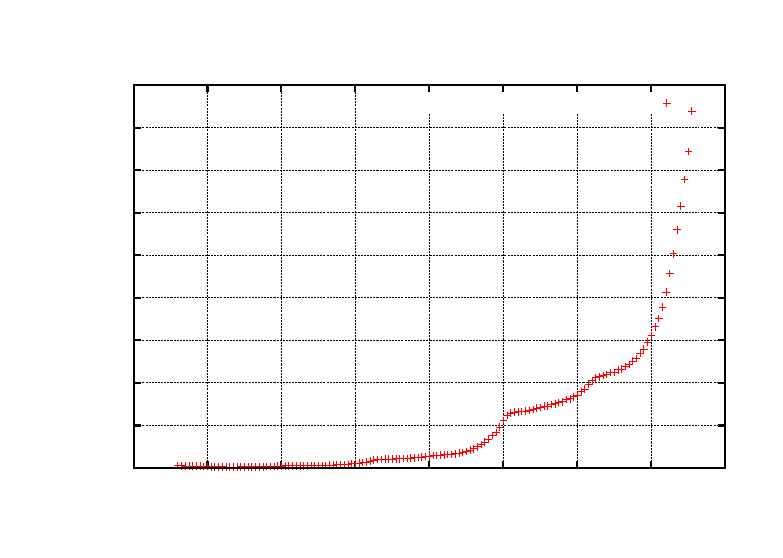
\includegraphics{abs}}%
    \gplfronttext
  \end{picture}%
\endgroup

	\caption{Absorptionsspektrum (380-700nm) von reinem Wasser. Daten aus einer spektroskopischen Untersuchung (1997). Nach: \cite{speck}}
	\label{fig:abs}
\end{figure}

\subsection{Nichtinvertierender Operationsverstärker}
\label{sec:teoverstaerker}
Dabei handelt es sich von der Grundschaltung her um einen Operationsverstärker.
Diese finden sehr viel Anwendung in allen möglichen Bereichen, zum Beispiel der Mess-und Regelungstechnik. 
Allgemeine Eigenschaften dieser Bauteile sind, eine sehr große Verstärkung von Eingangsignalen, sowie ein hoher Eingangs und dazu vergleichsweise geringer Ausgangswiderstand.
Das allgemeine Verstärkersymbol ist ein Dreieck in es werden darin auch die beiden
Eingänge mit + und - gekennzeichnet.
Der - Eingang wird als invertierender Eingang und 
der + Eingang als nicht invertierender Eingang bezeichnet.
Das eigentliche Bauteil des Verstärkers ist sehr komplex und es lohnt sich nicht hier 
weiter darauf einzugehen.
Entscheidend ist hier nur die Formel für den Verstärkungsfaktor $v$ für den verwendeten 
nichtinvertierenden Verstärkers. 
Für diese gilt
\begin{align}
 v = 1 + \frac{R_2}{R_1}~.\label{eq:verst}
\end{align}
Die Skizze zur Herleitung ist im Anhang zu finden (Abbildung \ref{fig:nicht}).
Wichtig ist also nur die für den jeweiligen Bedarf richtige Wahl des Widerstandsverhältnisses.
Eine weitere Eigenschaft des nichtinvertierenden Verstärkers ist, dass die Phase des Eingangs und Ausgangssignals gleich sind.
Diese Eigenschaft ist für das Echolot wichtig. Eine gute Einführung in das Thema Operationsverstärker findet man zum Beispiel in \cite{op}.


\subsection{Schichtung eines Sees}

Man unterscheidet drei Tiefenschichten eines Sees.
Diese haben alle verschiedene physikalische, chemische, sowie biologische Eigenschaften.
Die Grenzen zwischen diesen Schichten sind kontinuierlich und oftmals schwer zu unterscheiden. 
Dies gilt insbesondere für flache Seen.
Die oberste Schicht wird auch Epilimnion genannt. 
Im Sommer lagert sich dort warmes Wasser mit geringer Dichte ab.
Während dieser Zeit kommt es daher nur zu einem geringen Wasseraustausch mit tieferen Schichten, sodass in diesen immer weniger Sauerstoff zu finden ist.
Zudem findet effektiver Wärmeaustausch mit tieferen Schichten dann nur noch Aufgrund von vergleichsweise kleinen Strömungen statt.
Diese werden durch Wind oder im geringen Maße durch Sonneneinstrahlung erzeugt. 
Das Klima ist daher ein entscheidender Faktor für die Dicke dieser Schicht.
Diffusiver Wärmetransport hingegen ist ein sehr langsamer Prozess, so vergeht zum Beispiel etwa ein Monat für das Bilden einer etwa 1 m dicken Schicht vergleichsweise wärmeren Wassers.
Ab einer Tiefe von circa 10 m führt dies insgesamt zur Entstehung eines größeren Temperaturgradienten im Sommer und zur Entstehung der mittleren Schicht (Thermonokline).
Dabei handelt es sich um eine recht dünne Übergangschicht.
Diese trennt die obere Schicht von größeren Tiefen. 
\newline

%http://www.wiley-vch.de/books/sample/3527321314_c01.pdf
Das Epilimnion ist im Sommer die wärmste Schicht und besitzt den größten pH-Wert, da es hier zu Kontakt mit der Atmosphäre kommt.
In Folge dessen lösen sich Gase wie Kohlenstoffdioxid, sodass beispielsweise Kohlensäure entsteht.
Außerdem besitzt diese Schicht auch den größten Sauerstoffgehalt.
Hier sind auch die meisten phototrophen Planktonarten zu finden, da es ist der hellste Bereich des Sees ist.
Abgestorbenes Plankton lagert sich dann auf den Grund des Sees ab und steht anderen Lebewesen als Nahrung zur Verfügung.
\newline
Die unterste Schicht wird auch Hypolimnion genannt.
Im Sommer ist dies die kälteste Schicht und auch die mit dem geringsten Sauerstoffgehalt. 
Ganz grundsätzlich unterliegen diese Schichten jahreszeitlichen Schwankung in ihrer Dicke.
Es kommt dann im Herbst zu einer teilweisen Durchmischung zwischen Hypolimnion und dem Epilimnion, da sich das Wasser an der Oberfläche abkühlt und absinkt.
Im Winter, wenn die Außentemperaturen längere Zeit unter Null Grad gewesen sind, ist das Hypolimnion die wärmste Schicht, da Wasser mit einer Temperatur von 4 Grad am dichtesten ist. 
Im Extremfall liegt dann eine vollständige Durchmischung aller Schichten vor.
Aus diesem Grund ist eine (Temperatur-) Schichtung bei permanent gefrorenen Gewässern nicht vorzufinden.
\newline
In Grafik \ref{fig:schichtung} sind zur Veranschaulichung der Leitwert $C$, die Temperatur $T$ und das Sauerstoffgehaltsprofil des Arendsee (Sachsen Anhalt, Messung im September) dargestellt. 
Aufgrund der beinahe konstanten Temperatur im obersten sowie untersten Bereich kann man hier die drei oben geschilderten Schichten gut von einander trennen.
Insbesondere erkennt man den starken Temperaturgradienten im Metalimnion, das hier zwischen 8 und 15 m liegt. 
Näheres dazu findet man in der Quelle \cite{schicht}.
Das Kabel, welches in unserem Experiment den Logger mit der Sonde verbindet hat eine Länge von circa 8 m.
Es ist also zu erwarten, dass wir beim Vermessenen eines tiefen Sees grade an die Grenze des Epilimnions stoßen.


\begin{figure}[h]
	\centering
	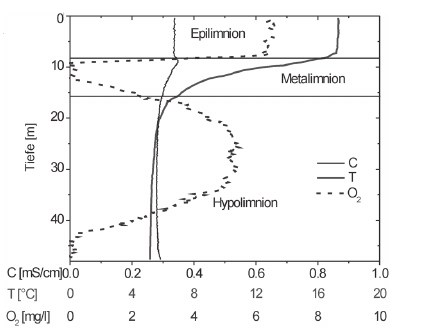
\includegraphics[width=0.6\textwidth]{schicht.png}
	\caption{Leitwert $C$, Temperatur $T$ und Sauerstoff $O_2$ des Arendsees im September. Grafik entnommen aus \cite{schicht} }
	\label{fig:schichtung}
\end{figure}



\subsection{Ortsbestimmung}
\label{sec:theoort}
Um den Ort des Bootes zu bestimmen, verwendeten wir ein Geodimeter (s. Abb. \ref{fig:geodimeter}).
Dieses sendet einen Laserstrahl in eine bestimmte Richtung aus und misst, sobald er reflektiert wird die Flugdauer.
Daraus bestimmt es die Entfernung.
Die Richtung wird durch die Stellung des beweglichen Kopfes ermittelt.
Dafür wird beim Einschalten eine Referenzrichtung eingestellt, anhand derer die Abweichung bestimmt wird.
Das Gerät kann nun die relative Position zu dem eigenen Standort in verschiedenen Darstellungsweisen ausgeben: Zylinderkoordinaten und kartesische Koordinaten.

Der Laser wird von einem Retroreflektor an einer Messstange reflektiert, welche mit an Bord genommen wird.
Ein Retroreflektor ist eine Anordnung von drei Spiegeln, welche jeweils im $90^\circ$-Winkel zueinander stehen.
Jeder einfallende Strahl wird so in die Herkunftsrichtung zurückgelenkt.\\
Als zweite mögliche Ortsbestimmung wird das GPS System verwendet, dass durch Triangulation von Signalen einiger Satelliten die Position bestimmt.
Diese Methode ist vergleichsweise ungenau mit einer Genauigkeit von $\pm5\si{\meter}$, aber im Vergleich zur Größe von Seen immer noch genau genug.
Die Implementierung dieser Methode wird im Kapitel \ref{sec:durchpos} weiter beschrieben.

Parallel zu dem direkten Speichern haben wir auch eine Smartphone-App erstellt, die ebenfalls die Position aufzeichnet (s. Kapitel \ref{sec:app}).


\subsection{Temperatur}
Die Temperatur wird mit einem Pt1000-Widerstand vermessen.
Der Name verrät, dass der Messfühler aus Platin ist und bei $0\si{\celsius}$ einen Widerstand von $R_0=1000\si{\ohm}$ hat.
Der Widerstand hängt nach \cite{Pt1000} so von der Temperatur $\vartheta>0\si{\celsius}$ ab
\begin{align}
	R(\vartheta)&=R_0\cdot\left(1 + A\vartheta + B\vartheta^2\right)~. \label{eq:Pt1000}
\end{align}
Diese Formel ist rein empirisch. 
Die zugehörigen Konstanten, welche in Eichmessungen ermittelt werden, findet man in Tabelle \ref{tab:Pt1000}.


Durch Umstellen erhält man eine Formel für die Temperatur in Grad Celsius
\begin{align}
 \vartheta = -\frac{A}{2 B} - \frac{1}{2 B \sqrt{R_0}} \sqrt{A^2 R_0  - 4 B R_0 + 4 B R    }\label{eq:temperapt1000}~.
\end{align}

\begin{table}[!htb]
	\centering
	\begin{tabular}{|c|c|}
		\hline
		R$_0$ & $1000 ~ \si{\ohm}$\\
		A   & $3.9083 \cdot 10^{-3} ~ \si{\celsius^{-1}}$\\
		B   & $-5.775 \cdot 10^{-7} ~ \si{\celsius^{-2}}$\\
		\hline
	\end{tabular}
	\caption{Kennwerte des Widerstandsthermometers}
	\label{tab:Pt1000}
\end{table}


\section{Durchführung}
\label{sec:durchfuehrung}

\subsection{Aufbau des Datenloggers}
Der Datenlogger ist speziell für diese Aufgabe entworfen und gebaut.
Die Basis für diesen ist das XMC4500 RelaxKit von der Firma Infoneon$^\copyright$ mit einem 32bit Mikrocontroller.
Dieser wurde mithilfe der Software Dave$^\copyright$ von der gleichen Firma programmiert.
Die Bedienung erfolgt über ein Interface aus drei Tastern und eine LCD Display.
Das Display dient nicht nur der Steuerung, sondern zeigt auch im Sekundentakt die Momentanen Messwerte an.
Zur Bestimmung der am Controller anliegenden Spannung wird ein integrierter Analog Digital Converter (ADC) verwendet.
Dieser berechnet die Spannung über ein iteratives Verfahren, in dem er die anliegende Spannung mit einer Referenzspannung vergleicht.
Die Referenzspannung wird bei jedem Schritt halbiert oder um die Hälfte erhöht je nachdem, ob die zu messende Spannung kleiner oder größer ist.
Der ADC hat eine Auflösung von 12bit, wie im Datenblatt \cite[7]{XMCRelaxkit} zu lesen ist, somit hat das Verfahren auch 12 Schritte.
Die Referenzspannung liegt bei 3.3\si{\volt}, welche vom Board intern bereitgestellt wird.
Diese Spannung ist auch die Maximalspannung, die an einen Pin des Mikrocontrollers angelegt werden darf, ohne ihn zu zerstören.
Aus diesem Verfahren ergibt sich bei 12bit eine minimal von Null verschiedene Spannung von $B=\frac{3.3\si{\volt}}{2^{12}}=8.06\times10^{-4}\si{\volt}$, welche als Bereichsbreite $B$ bezeichnet wird.
Somit kann die Spannung aus dem ausgegebenen ADCWert über die Bereichsbreite berechnet werden
\begin{align}
	U=\text{ADCWert}\cdot B~.\label{eq:ADCwert}
\end{align}
Die Daten werden in Form einer ASCII Datei auf einer SD-Karte gespeichert um sie später am Computer leichter in einem Plotprogramm bearbeiten zu können.
Dies sorgt aber für ein größeres Datenaufkommen.
Jede Datei trägt, zur besseren Identifikation, den aktuellen Monat, Tag, Stunde und Minute als Namen (MMDDhhmm.dat).
In der Datei wird die Zeit in Millisekunden, die ADCWerte von Temperatur, Photodiode und Druck, sowie die berechneten Werte der Temperatur, Intensität, Druck und Tiefe berechnet aus dem aktuellen Luftdruck eingetragen.
Der aktuelle Luftdruck kann über das Einstellungsmenü direkt am Logger geändert werden.\\
Die Zeit wird anhand der aktuellen Zeit und jedem weiteren Zeitschritt bestimmt.
Das Programm kann von 10 bis zu maximal 500 Werten pro Sekunde aufnehmen, welche in den Einstellungen während der Laufzeit geändert werden können.
Der Zeitschritt wird abhängig von der Wertfrequenz berechnet und eingetragen.\\
Für die Sensoren werden verschiedene Schaltungen verwendet, die im Folgenden näher erläutert werden.
Bei allen Schaltungen ist zu beachten, dass in allen Fällen die Massen gekoppelt sind.
Die Spannungen werden von jedem Sensor über ein geschirmtes Kabel übertragen.
In dem Kabel sind zu dem noch alle Aderpaare gegen die anderen Paare abgeschirmt.


\subsubsection{Temperaturmessung}
Für die Messung der Temperatur wird mit einem Pt1000 Temperaturwiderstand gearbeitet.
Dieser benötigt eine spezielle Beschaltung, da durch ihn nur ein geringer Strom fließen darf.
Aus diesem Grund muss die am Pt1000 abfallende Spannung noch verstärkt werden.
Dies geschieht mithilfe eines nicht-invertierenden Verstärkers wie im Kapitel \ref{sec:teoverstaerker} beschrieben.
Mit der Formel \eqref{eq:verst} ergibt sich bei der in der Abbildung \ref{fig:PT1000Schaltung} gezeigte Beschaltung eine Verstärkungsfaktor von 11.
Dieser Wert verstärkt somit die etwa 200\si{\milli\volt} auf etwa 2\si{\volt}, was gut im Messbereiche des ADCs liegt.\\
Aus dem in der Abbildung \ref{fig:PT1000Schaltung} zu sehendem Widerstandsnetzwerk leitet sich die Formel
\begin{align}
	R_\text{Pt1000}=\frac{R_1\cdot U_\text{ADC}}{3.3\si{\volt}-U_\text{ADC}}
\end{align}
ab, wobei $U_\text{ADC}$ die Spannung ist, welche mit der Formel \eqref{eq:ADCwert} aus dem ADCWert berechnet wird.
Zur anschließenden Berechnung der Temperatur aus den gemessenen Widerständen wird die Formel \eqref{eq:temperapt1000} verwendet.\\
Der Sensor ist zwecks Wasserdichtigkeit mit einem dünnen Film Klebstoff beschichtet.
Dieser sollte nur die Reaktionszeit beeinflussen.

\subsubsection{Lichtmessung}
Für die Lichtmessung wird eine Photodiode als intensitätsabhängige Stromquelle verwendet.
Die Schaltung ist in der Abbildung \ref{fig:PhotodiodeSchaltung} zu sehen.
Der Stromkreis besteht aus der Photodiode als Stromquelle und einem Widerstand, um den Strom in eine Messbare Spannung zu wandeln.
Da in den See nicht viel Licht eintritt, wird die sich ergebene Spannung noch über einen nicht-invertierenden Verstärker nach der Gleichung \ref{eq:verst} mit einem Faktor 11 Verstärkt.
Die Spannung wird dann wieder mit der Gleichung \eqref{eq:ADCwert} berechnet.\\
Um die Absorption in verschiedenen Spektren zu Messen hat die Messsonde eine Blaue und eine Infrarote LED
mit mittleren Wellenlängen von $\lambda_\text{Blau}=460\si{\nano\meter}$ \cite[2]{BLAUDatenblatt} und $\lambda_\text{IR}=940\si{\nano\meter}$ \cite[4]{IRDatenblatt}.
Die LEDs werden ebenfalls von der boardinternen Spannungsquelle versorgt und wie in der Abbildung \ref{fig:LEDSchaltung} zu sehen mit entsprechenden Vorwiderständen beschaltet.
Um die LEDs von dem Umgebungslicht zu unterscheiden werden diese gepulst, sie werden im bestimmten Zyklen ein und aus geschaltet.
Die Frequenz mit der die LEDs nacheinander ein und aus geschaltet werden heißt Umschaltfrequenz und ist von 0\si{\hertz} bis 20\si{\hertz} durchschaltbar.
Im Programm werden die Linien von den jeweiligen LEDs und den Phasen ohne LED-Betrieb getrennt gespeichert.

\subsubsection{Druckmessung}
\label{sec:durchdruck}
Der Druck wird durch einen Absolutdrucksensor in einer Messbrücke bestimmt.
Die Schaltung wurde von der Geophysik bereitgestellt und direkt an dem Pin 14.2 am Board angeschlossen.
Zu dem muss die Masse von der externen Schaltung mit der Masse des Boards gekoppelt werden.
Die Messbrücke ist mit einem Potentiometer bei einer Spannung von 1\si{\volt} auf einen Druck von 1001hPa geeicht.
Bei der Messbrücke handelt es sich um  eine Wheatstone'sche Brücke, die bereits vom Werk aus geeicht ist.
Die ausgegebene Spannung ist somit proportional zum angewandten Druck.
Der Luftdruck liegt bei etwa 1000hPa und in einer Tiefe von 10\si{\meter} hat sich der Druck nach der Gleichung \eqref{eq:d} um 1000hPa erhöht, und damit auch die Spannung um 1\si{\volt}.
Somit liegt der Spannungsbereich in dem akzeptablen Bereich des ADC.\\
Die Messbrücke ist in ein wasserdichtes Gehäuse gebaut und wird über ein externes Kabel mit einer eigenen Platine und eigener Spannungsversorgung geführt.
Somit ist die Druckmessung vollkommen von den anderen Messungen getrennt und wird nicht von diesen beeinflusst.

\subsubsection{Echolotmessung}
Mithilfe von zwei Piezokristallen wird eine Echolotmessung realisiert.
Die Kristalle haben eine Resonanzfrequenz von 40\si{\kilo\hertz} und liegen somit im Ultraschallbereich.
Das Senderkristall wird mithilfe von PWM (Puls Width Modulation) mit einem Signal von maximal +3.3\si{\volt} versorgt, um diese Maximalspannung zu erhöhen wird das Kristall über ein MOSFET-Transistor an +24\si{\volt} betrieben.
Um die Tiefe zu Messen, muss ein klar definiertes Signal ausgesendet werden, hierzu werden 20 Schwingungen auf das Senderkristall gegeben.\\
Das Empfängerkristall wird über einen Verstärker direkt an den ADC angeschlossen.
Für die Messung der Tiefe wird die Laufzeit der Wellen vom Aussenden bis zum Empfangen gemessen und daraus die Entfernung berechnet.
Die Entfernung wird nach dem Gesetzen aus dem Kapitel \ref{sec:theschallgeschw} berechnet.
Zur Bestimmung der Bodenbeschaffenheit wird zudem das ganze ausgesendete Signal aufgezeichnet und anschließend analysiert.

\subsection{Positionsbestimmung via GPS und Geodimeter}
\label{sec:durchpos}
Die Bestimmung der Position wird zum einen mithilfe eines Geodimeters durchgeführt.
Dieses berechnet, wie im Kapitel\ref{sec:theoort} beschrieben, die Position durch eine genaue Berechnung der Entfernung und des Winkels mithilfe eines Lasers und einem Retroreflektor.
Diese Messmethode ist sehr genau, benötigt aber zwei Teams, eines das an Land das Geodimeter bedient, sowie die Koordinaten notiert und eines, dass auf dem Boot den Retroreflektor positioniert.\\
Als Alternative hierzu wird ein GPS in den Datenlogger implementiert, welches bei jeder Messung die aktuellen globalen Koordinaten an die letzte Stelle der Messdatei schreibt.
Hierzu wird ein GPS von Garmin$^{\copyright}$ verwendet, welches in der Geophysik vorhanden war.
Dieses besitzt eine RS232 Schnittstelle, welche mithilfe eines selbstgebauten Pegelkonverters die $\pm6\si{\volt}$ auf TTL Signale mit einem maximalen Pegel von 3.3\si{\volt} und einem minimalen Pegel von 0\si{\volt} konvertiert.
Dies geschieht über 5 Dioden und einem Pulldownwiderstand, um eine kleine Last zu erzeugen, die das Signal nicht verzerrt.
Anschließend werden die Daten vom Mikrocontroller über eine UART Schnittstelle bei einer Baudrate von 9600$~$Baud eingelesen.
Das GPS sendet die aktuellen Koordinaten mit der aktuellen Atomuhrzeit als ASCII Text jede Sekunde an den Logger.
Mithilfe der Zeit kann die RTC (Realtimeclock) des Boardes einmalig auf die GPS-Zeit eingestellt werden.

\subsection{Messdurchführung}

Zur Vermessung eines Sees ist es notwendig, zunächst den Bereich, den man vermessen möchte sinnvoll einzuschränken und sich eine Rasterung zu überlegen.
Dabei ist zu bedenken, dass für jeden Messpunkt ca. 3-5min eingerechnet werden müssen.
Auch müssen die Positionen, sofern sie mit dem Geodimeter ermittelt werden sollen, alle von einem Punkt am Ufer aus sichtbar sein.
Man könnte zwar das Geodimeter umstellen, jedoch würde dies zu einer enorm vergrößerten Unsicherheit des Ortes führe.

Die eigentliche Messung besteht darin, dass der Ruderer an einer Stelle anhält, den Messstab für das Geodimeter hochhält und ausrichtet.
Wird die Einzelmessung der App gleichzeitig mit dem Datenlogger gestartet, so wird zu den GPS-Daten der App gleich der Dateiname der Messreihe gespeichert.
Ist nun die Messung gestartet, so wird die Sonde langsam ins Wasser gelassen.
Um eine signifikante Menge an Datenpunkten für alle Tiefen zu bekommen, darf man die Sonde nur mit einer Sinkgeschwindigkeit von höchstens 10cm/s herunterlassen.
Erreicht die Sonde den Boden, so muss die Messung beendet werden, da sich sonst gegebenenfalls Schlamm um die Sensoren legt.
Kommt das Gewicht nicht auf dem Boden an, so kann die Sonde wieder nach oben gezogen werden um die doppelte Anzahl an Messwerten für die jeweilige Tiefe zu bekommen.

Erreicht die Sonde in diesem Fall wieder die Oberfläche, so wird die Messung beendet.
Dies ist notwendig, da der Lichtsensor an der Oberfläche durch die Sonneneinstrahlung eine zu hohe Spannung liefert und so den ADC übersteuert.

\subsection{Smartphone-App}
\label{sec:app}
Da bei der ersten Messung schon das Abfahren des relativ kleinen Göttinger Kiessees in einem regelmäßigen Raster nicht leicht war, haben wir eine App für das Smartphone erstellt.
Das GPS-Modul des Smartphones liefert die aktuelle Position und stellt sie auf einer Karte dar.
Nun gibt es zwei Möglichkeiten:
\begin{itemize}
	\item Multi-Messung: Die Position wird ständig getrackt.
		Sobald sie sich verändert, wird diese in eine Datei geschrieben.
	\item Einzelmessung: Dies kann parallel zu der Multi-Messung passieren.
		Hierbei wird nur auf Knopfdruck auf den Button "`Einzelmessung"' ein einzelner Ort in eine andere Datei geschrieben.
		Außerdem wird die Position auf der Karte mit einer Stecknadel markiert und um die Position wird ein Radius eingezeichnet, der sich über einen Schieberegler einstellen lässt.
		Dies hat den Vorteil, dass man variabel die Rasterung anpassen kann.
\end{itemize}

Die App zeigt (wie in Abb. \ref{fig:appDetail} zu sehen) auch die Anzahl der aufgenommenen Datenpunkte an und die beiden Dateien, welche bei den Messungen angelegt werden.

Wurde die Messung an einem Ort nun beendet, kann man einfach so lange in eine Richtung fahren, bis man den roten Kreis um den letzten Datenpunkt erreicht hat.
Im Verlauf der Messung wird nun der ganze See systematisch mit den Kreisen überdeckt.

Am Ende des Messtages kann mit dem Knopf "`Senden"' nun eine Tabelle (s. Abb. \ref{fig:appTabelle}) geöffnet werden, welche die vorhandenen Dateien anzeigt.
Tippt man nun auf eine der Zeilen, so wird eine Mail erstellt, die schon voreingestellt die Mailadressen, Betreff und Inhalt, sowie die angehängte Datei besitzt.
Diese kann nun bequem mit einem Tippen versandt werden.


\begin{figure}[h]
  \centering
  \subfigure[Einzelne Datenpunkte an einer Stelle des Sees.\label{fig:appDetail}]
  {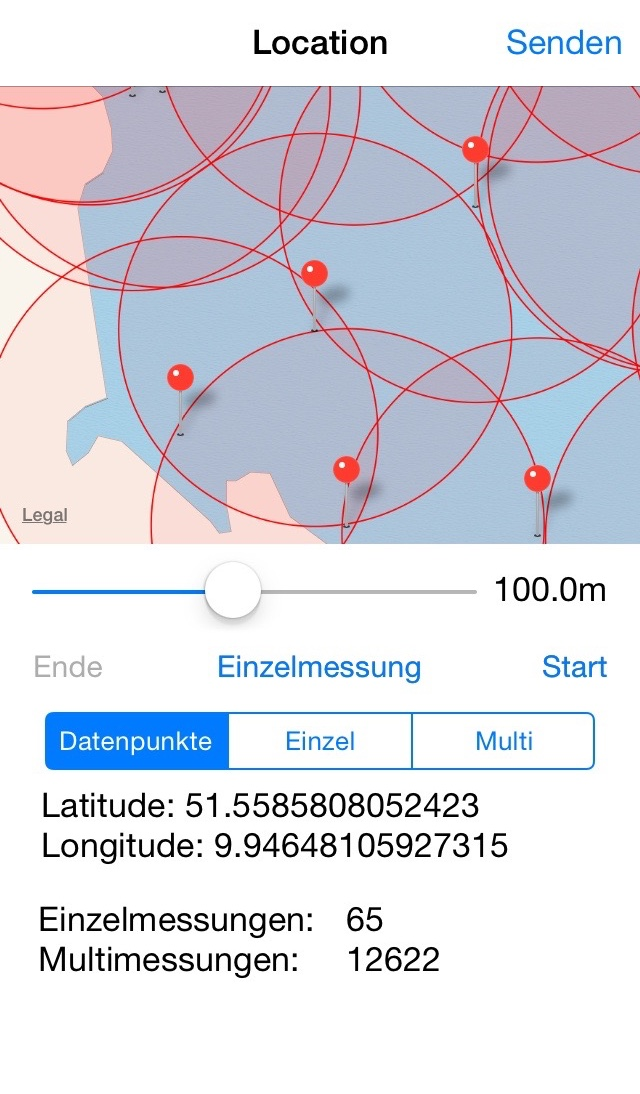
\includegraphics[width=0.32\textwidth]{Fotos/AppSeeDetail}}
  \hfill
  \subfigure[Übersicht über alle aufgenommenen Messpunkte in der App.\label{fig:appGesamt}]
  {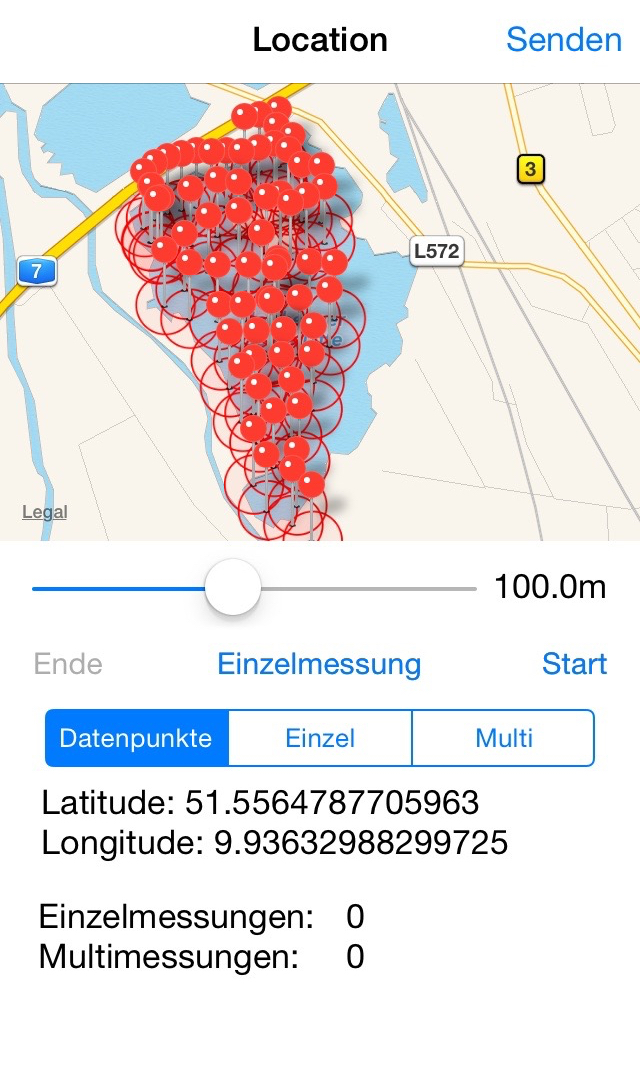
\includegraphics[width=0.32\textwidth]{Fotos/AppSeeKomplett}}
  \hfill
  \subfigure[Auswahl der zu versendenden Datei.\label{fig:appTabelle}]
  {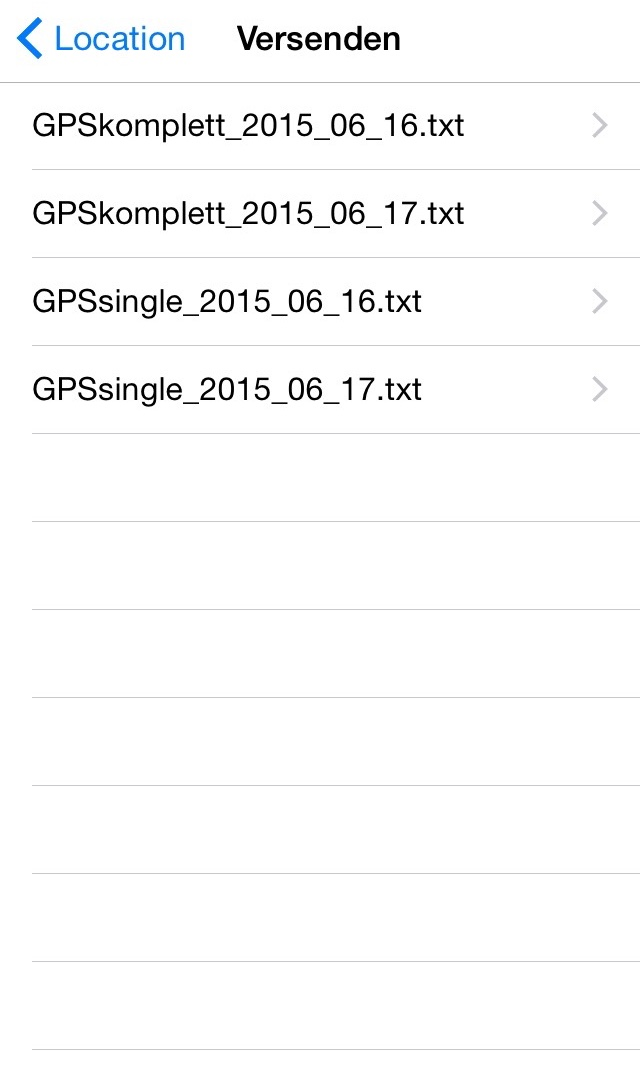
\includegraphics[width=0.32\textwidth]{Fotos/AppVersenden}}
  \caption{Screenshots der App.}
  \label{fig:appScreenshots}
\end{figure}


\section{Auswertung}
\label{sec:auswertung}

Unser eigentlicher Plan sah vor, den Seeburger See zu vermessen.
Dieser ist bis zu 4.2 Meter tief \footnote{\url{www.nlwkn.niedersachsen.de/download/58239/Seeburger\_See.pdf}, S.7}.
Dementsprechend wählten wir unsere Kabellängen.
Da dieser See jedoch auf Grund von Granatenfunden aus dem 2. Weltkrieg vom 25.05. bis zum 26.06.15 gesperrt war, mussten wir auf andere Seen in der Region ausweichen.\\
So haben wir am 10. Juni am Göttinger Kiessee unsere ersten Messdaten aufgenommen.
Da dieser viel kleiner und nur maximal 2.2 Meter tief ist, erwarteten wir nicht, dort auf interessante Phänomene zu stoßen.
Jedoch konnten wir so die Sonde testen und wir haben viele Probleme während des Messprozesses entdeckt, wie die Effekte, welche von Schlamm an den Sensoren herrühren.\\
Eine Woche später, also am 17.06., haben wir dann auf dem Großen See bei Northeim gemessen.
Um mehr Messdaten über die Lichtstreuung zu bekommen, setzten wir bei dieser Messung die Umschaltfrequenz der LEDs von $2\,$Hz auf $10\,$Hz.
Beim Testen unseres Messgeräts am Morgen stellten wir jedoch fest, dass man drei verschiedene "`Temperaturkurven"' sieht, also immer wieder Sprünge in den berechneten Temperaturdaten.
Dies liegt an dem An-/Ausschalten der beiden LEDs.
Eine genauere Erklärung findet sich im Abschnitt \ref{sec:DiskTemp}.
Diesen Effekt sieht man jedoch nicht bei  den ersten Messdaten, da dort die Frequenz geringer war.
Allerdings springen die Temperaturwerte von Messreihe zu Messreihe.
Dies ist schlecht, da man somit manchmal überhaupt keine richtigen Daten hat, die man mit anderen vergleichen kann.

\subsection{Ortsbestimmung}
\label{sec:ausort}
Unsere Befürchtung, dass das GPS-Signal zu ungenau ist, stellte sich als falsch heraus.
Wir nutzten bei der zweiten Messung gleichzeitig einen GPS-Logger und die selbstgeschriebene Handy-App.
Durch Vergleich der beiden Messdaten erkennt man, dass sie sehr gut miteinander übereinstimmen.
Dies ist vielleicht auch zu erwarten, da beide ähnliche Signale bekamen.

Der GPS-Logger zeigte die Genauigkeit auf dem Display an, welche fast immer 3m betrug.
Diese hohe Genauigkeit, welche sich unter "`Normalbedingungen"' nur selten erreichen lässt, wird dadurch erklärt, dass wir auf einer weiten Fläche ohne große Hindernisse waren.
Somit gab es nichts, was die Signale der Satelliten reflektieren oder blockieren konnte.


In Abb. \ref{fig:tiefeGoe} sind die Tiefen an den jeweiligen Messpunkten am Göttinger Kiessee aufgetragen.
Diese wurden mit dem Geodimeter bestimmt und die gestrichelten Linien verbinden die Messpunkte miteinander.
Dabei ist zu erkennen, dass die Fahrt
Als Vergleich sind die Daten, die wir mit einer kommerziellen App aufgenommen haben, in Abb. \ref{fig:GPSGoe} aufgetragen.
Diese wurden durchgehend aufgezeichnet, jedoch kann man an den Umkehrpunkten erkennen, dass die Positionen ungefähr übereinstimmen.
Es ist zu erkennen, dass wir kein regelmäßiges Raster abgefahren sind.

In Abb. \ref{fig:GPSNort} kann man erkennen, dass wir in Northeim mit der Unterstützung der Smart\-phone-App wesentlich besser gefahren sind.
Dass wir die östliche Seite des Sees nicht befahren haben, liegt daran, dass dort noch aktiv Kies abgebaut wird.
Daher ist das Befahren dort verboten.

%\begin{figure}[!h]
%\centering
%\input{goekiessee/kartegoe.tex}
%\caption{positionen der messungen am 10.6.2015 auf dem göttinger kiessee gemessen mit dem geodimeter.}
%\label{fig:einzelgpsgoe}
%\end{figure}
\begin{figure}[!h]
\centering
% GNUPLOT: LaTeX picture with Postscript
\begingroup
  \makeatletter
  \providecommand\color[2][]{%
    \GenericError{(gnuplot) \space\space\space\@spaces}{%
      Package color not loaded in conjunction with
      terminal option `colourtext'%
    }{See the gnuplot documentation for explanation.%
    }{Either use 'blacktext' in gnuplot or load the package
      color.sty in LaTeX.}%
    \renewcommand\color[2][]{}%
  }%
  \providecommand\includegraphics[2][]{%
    \GenericError{(gnuplot) \space\space\space\@spaces}{%
      Package graphicx or graphics not loaded%
    }{See the gnuplot documentation for explanation.%
    }{The gnuplot epslatex terminal needs graphicx.sty or graphics.sty.}%
    \renewcommand\includegraphics[2][]{}%
  }%
  \providecommand\rotatebox[2]{#2}%
  \@ifundefined{ifGPcolor}{%
    \newif\ifGPcolor
    \GPcolortrue
  }{}%
  \@ifundefined{ifGPblacktext}{%
    \newif\ifGPblacktext
    \GPblacktexttrue
  }{}%
  % define a \g@addto@macro without @ in the name:
  \let\gplgaddtomacro\g@addto@macro
  % define empty templates for all commands taking text:
  \gdef\gplbacktext{}%
  \gdef\gplfronttext{}%
  \makeatother
  \ifGPblacktext
    % no textcolor at all
    \def\colorrgb#1{}%
    \def\colorgray#1{}%
  \else
    % gray or color?
    \ifGPcolor
      \def\colorrgb#1{\color[rgb]{#1}}%
      \def\colorgray#1{\color[gray]{#1}}%
      \expandafter\def\csname LTw\endcsname{\color{white}}%
      \expandafter\def\csname LTb\endcsname{\color{black}}%
      \expandafter\def\csname LTa\endcsname{\color{black}}%
      \expandafter\def\csname LT0\endcsname{\color[rgb]{1,0,0}}%
      \expandafter\def\csname LT1\endcsname{\color[rgb]{0,1,0}}%
      \expandafter\def\csname LT2\endcsname{\color[rgb]{0,0,1}}%
      \expandafter\def\csname LT3\endcsname{\color[rgb]{1,0,1}}%
      \expandafter\def\csname LT4\endcsname{\color[rgb]{0,1,1}}%
      \expandafter\def\csname LT5\endcsname{\color[rgb]{1,1,0}}%
      \expandafter\def\csname LT6\endcsname{\color[rgb]{0,0,0}}%
      \expandafter\def\csname LT7\endcsname{\color[rgb]{1,0.3,0}}%
      \expandafter\def\csname LT8\endcsname{\color[rgb]{0.5,0.5,0.5}}%
    \else
      % gray
      \def\colorrgb#1{\color{black}}%
      \def\colorgray#1{\color[gray]{#1}}%
      \expandafter\def\csname LTw\endcsname{\color{white}}%
      \expandafter\def\csname LTb\endcsname{\color{black}}%
      \expandafter\def\csname LTa\endcsname{\color{black}}%
      \expandafter\def\csname LT0\endcsname{\color{black}}%
      \expandafter\def\csname LT1\endcsname{\color{black}}%
      \expandafter\def\csname LT2\endcsname{\color{black}}%
      \expandafter\def\csname LT3\endcsname{\color{black}}%
      \expandafter\def\csname LT4\endcsname{\color{black}}%
      \expandafter\def\csname LT5\endcsname{\color{black}}%
      \expandafter\def\csname LT6\endcsname{\color{black}}%
      \expandafter\def\csname LT7\endcsname{\color{black}}%
      \expandafter\def\csname LT8\endcsname{\color{black}}%
    \fi
  \fi
  \setlength{\unitlength}{0.0500bp}%
  \begin{picture}(7200.00,5040.00)%
    \gplgaddtomacro\gplbacktext{%
      \csname LTb\endcsname%
      \put(2037,704){\makebox(0,0)[r]{\strut{} 0}}%
      \put(2037,1111){\makebox(0,0)[r]{\strut{} 5e+06}}%
      \put(2037,1518){\makebox(0,0)[r]{\strut{} 1e+07}}%
      \put(2037,1925){\makebox(0,0)[r]{\strut{} 1.5e+07}}%
      \put(2037,2332){\makebox(0,0)[r]{\strut{} 2e+07}}%
      \put(2037,2740){\makebox(0,0)[r]{\strut{} 2.5e+07}}%
      \put(2037,3147){\makebox(0,0)[r]{\strut{} 3e+07}}%
      \put(2037,3554){\makebox(0,0)[r]{\strut{} 3.5e+07}}%
      \put(2037,3961){\makebox(0,0)[r]{\strut{} 4e+07}}%
      \put(2037,4368){\makebox(0,0)[r]{\strut{} 4.5e+07}}%
      \put(2037,4775){\makebox(0,0)[r]{\strut{} 5e+07}}%
      \put(2169,484){\makebox(0,0){\strut{}-2.5e+07}}%
      \put(2576,484){\makebox(0,0){\strut{}-2e+07}}%
      \put(2983,484){\makebox(0,0){\strut{}-1.5e+07}}%
      \put(3390,484){\makebox(0,0){\strut{}-1e+07}}%
      \put(3797,484){\makebox(0,0){\strut{}-5e+06}}%
      \put(4205,484){\makebox(0,0){\strut{} 0}}%
      \put(4612,484){\makebox(0,0){\strut{} 5e+06}}%
      \put(5019,484){\makebox(0,0){\strut{} 1e+07}}%
      \put(5426,484){\makebox(0,0){\strut{} 1.5e+07}}%
      \put(5833,484){\makebox(0,0){\strut{} 2e+07}}%
      \put(6240,484){\makebox(0,0){\strut{} 2.5e+07}}%
      \put(739,2739){\rotatebox{-270}{\makebox(0,0){\strut{}y [m]}}}%
      \put(4204,154){\makebox(0,0){\strut{}x [m]}}%
    }%
    \gplgaddtomacro\gplfronttext{%
      \csname LTb\endcsname%
      \put(5253,1097){\makebox(0,0)[r]{\strut{}GPS}}%
      \csname LTb\endcsname%
      \put(5253,877){\makebox(0,0)[r]{\strut{}Geodimeter}}%
    }%
    \gplbacktext
    \put(0,0){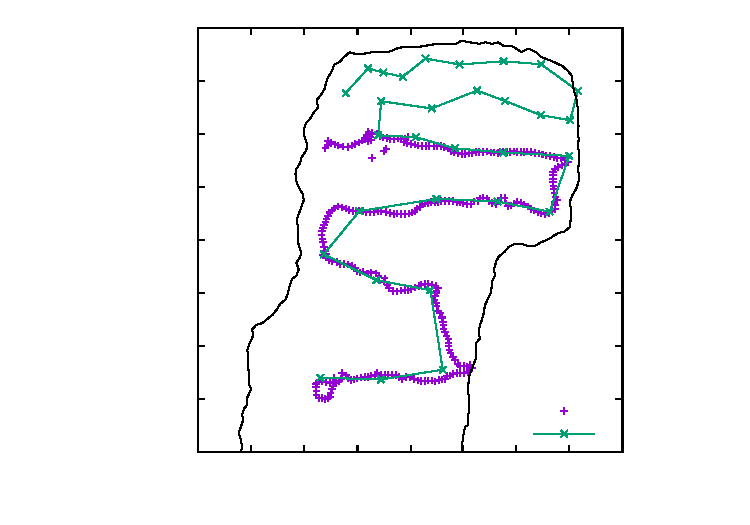
\includegraphics{GPSvsGeo}}%
    \gplfronttext
  \end{picture}%
\endgroup

\caption{Position des Bootes laut GPS-Signal verglichen mit den Geodimeter Messorten in Göttingen.}
\label{fig:GPSGoe}
\end{figure}

\begin{figure}[!h]
	\centering
	%\resizebox{\linewidth}{!}{% GNUPLOT: LaTeX picture with Postscript
\begingroup
  \makeatletter
  \providecommand\color[2][]{%
    \GenericError{(gnuplot) \space\space\space\@spaces}{%
      Package color not loaded in conjunction with
      terminal option `colourtext'%
    }{See the gnuplot documentation for explanation.%
    }{Either use 'blacktext' in gnuplot or load the package
      color.sty in LaTeX.}%
    \renewcommand\color[2][]{}%
  }%
  \providecommand\includegraphics[2][]{%
    \GenericError{(gnuplot) \space\space\space\@spaces}{%
      Package graphicx or graphics not loaded%
    }{See the gnuplot documentation for explanation.%
    }{The gnuplot epslatex terminal needs graphicx.sty or graphics.sty.}%
    \renewcommand\includegraphics[2][]{}%
  }%
  \providecommand\rotatebox[2]{#2}%
  \@ifundefined{ifGPcolor}{%
    \newif\ifGPcolor
    \GPcolortrue
  }{}%
  \@ifundefined{ifGPblacktext}{%
    \newif\ifGPblacktext
    \GPblacktexttrue
  }{}%
  % define a \g@addto@macro without @ in the name:
  \let\gplgaddtomacro\g@addto@macro
  % define empty templates for all commands taking text:
  \gdef\gplbacktext{}%
  \gdef\gplfronttext{}%
  \makeatother
  \ifGPblacktext
    % no textcolor at all
    \def\colorrgb#1{}%
    \def\colorgray#1{}%
  \else
    % gray or color?
    \ifGPcolor
      \def\colorrgb#1{\color[rgb]{#1}}%
      \def\colorgray#1{\color[gray]{#1}}%
      \expandafter\def\csname LTw\endcsname{\color{white}}%
      \expandafter\def\csname LTb\endcsname{\color{black}}%
      \expandafter\def\csname LTa\endcsname{\color{black}}%
      \expandafter\def\csname LT0\endcsname{\color[rgb]{1,0,0}}%
      \expandafter\def\csname LT1\endcsname{\color[rgb]{0,1,0}}%
      \expandafter\def\csname LT2\endcsname{\color[rgb]{0,0,1}}%
      \expandafter\def\csname LT3\endcsname{\color[rgb]{1,0,1}}%
      \expandafter\def\csname LT4\endcsname{\color[rgb]{0,1,1}}%
      \expandafter\def\csname LT5\endcsname{\color[rgb]{1,1,0}}%
      \expandafter\def\csname LT6\endcsname{\color[rgb]{0,0,0}}%
      \expandafter\def\csname LT7\endcsname{\color[rgb]{1,0.3,0}}%
      \expandafter\def\csname LT8\endcsname{\color[rgb]{0.5,0.5,0.5}}%
    \else
      % gray
      \def\colorrgb#1{\color{black}}%
      \def\colorgray#1{\color[gray]{#1}}%
      \expandafter\def\csname LTw\endcsname{\color{white}}%
      \expandafter\def\csname LTb\endcsname{\color{black}}%
      \expandafter\def\csname LTa\endcsname{\color{black}}%
      \expandafter\def\csname LT0\endcsname{\color{black}}%
      \expandafter\def\csname LT1\endcsname{\color{black}}%
      \expandafter\def\csname LT2\endcsname{\color{black}}%
      \expandafter\def\csname LT3\endcsname{\color{black}}%
      \expandafter\def\csname LT4\endcsname{\color{black}}%
      \expandafter\def\csname LT5\endcsname{\color{black}}%
      \expandafter\def\csname LT6\endcsname{\color{black}}%
      \expandafter\def\csname LT7\endcsname{\color{black}}%
      \expandafter\def\csname LT8\endcsname{\color{black}}%
    \fi
  \fi
  \setlength{\unitlength}{0.0500bp}%
  \begin{picture}(7200.00,5040.00)%
    \gplgaddtomacro\gplbacktext{%
      \csname LTb\endcsname%
      \put(2503,1601){\makebox(0,0)[l]{\strut{}N}}%
    }%
    \gplgaddtomacro\gplfronttext{%
      \csname LTb\endcsname%
      \put(3945,1259){\makebox(0,0)[r]{\strut{}max. Tiefe}}%
      \csname LTb\endcsname%
      \put(2400,800){\makebox(0,0){\strut{}-400}}%
      \csname LTb\endcsname%
      \put(2743,800){\makebox(0,0){\strut{}-200}}%
      \csname LTb\endcsname%
      \put(3086,800){\makebox(0,0){\strut{} 0}}%
      \csname LTb\endcsname%
      \put(3429,800){\makebox(0,0){\strut{} 200}}%
      \csname LTb\endcsname%
      \put(3771,800){\makebox(0,0){\strut{} 400}}%
      \csname LTb\endcsname%
      \put(4114,800){\makebox(0,0){\strut{} 600}}%
      \csname LTb\endcsname%
      \put(4457,800){\makebox(0,0){\strut{} 800}}%
      \csname LTb\endcsname%
      \put(4800,800){\makebox(0,0){\strut{} 1000}}%
      \put(3600,470){\makebox(0,0){\strut{}$x$ [m]}}%
      \csname LTb\endcsname%
      \put(2228,1086){\makebox(0,0)[r]{\strut{}-1600}}%
      \csname LTb\endcsname%
      \put(2228,1429){\makebox(0,0)[r]{\strut{}-1400}}%
      \csname LTb\endcsname%
      \put(2228,1773){\makebox(0,0)[r]{\strut{}-1200}}%
      \csname LTb\endcsname%
      \put(2228,2116){\makebox(0,0)[r]{\strut{}-1000}}%
      \csname LTb\endcsname%
      \put(2228,2459){\makebox(0,0)[r]{\strut{}-800}}%
      \csname LTb\endcsname%
      \put(2228,2801){\makebox(0,0)[r]{\strut{}-600}}%
      \csname LTb\endcsname%
      \put(2228,3144){\makebox(0,0)[r]{\strut{}-400}}%
      \csname LTb\endcsname%
      \put(2228,3487){\makebox(0,0)[r]{\strut{}-200}}%
      \csname LTb\endcsname%
      \put(2228,3831){\makebox(0,0)[r]{\strut{} 0}}%
      \csname LTb\endcsname%
      \put(2228,4174){\makebox(0,0)[r]{\strut{} 200}}%
      \put(1502,2630){\rotatebox{-270}{\makebox(0,0){\strut{}$y$ [m]}}}%
      \put(5112,1086){\makebox(0,0)[l]{\strut{}-8}}%
      \put(5112,1472){\makebox(0,0)[l]{\strut{}-7}}%
      \put(5112,1858){\makebox(0,0)[l]{\strut{}-6}}%
      \put(5112,2244){\makebox(0,0)[l]{\strut{}-5}}%
      \put(5112,2630){\makebox(0,0)[l]{\strut{}-4}}%
      \put(5112,3016){\makebox(0,0)[l]{\strut{}-3}}%
      \put(5112,3402){\makebox(0,0)[l]{\strut{}-2}}%
      \put(5112,3788){\makebox(0,0)[l]{\strut{}-1}}%
      \put(5112,4174){\makebox(0,0)[l]{\strut{} 0}}%
      \put(5442,2630){\rotatebox{-270}{\makebox(0,0){\strut{}$z$ [m]}}}%
    }%
    \gplbacktext
    \put(0,0){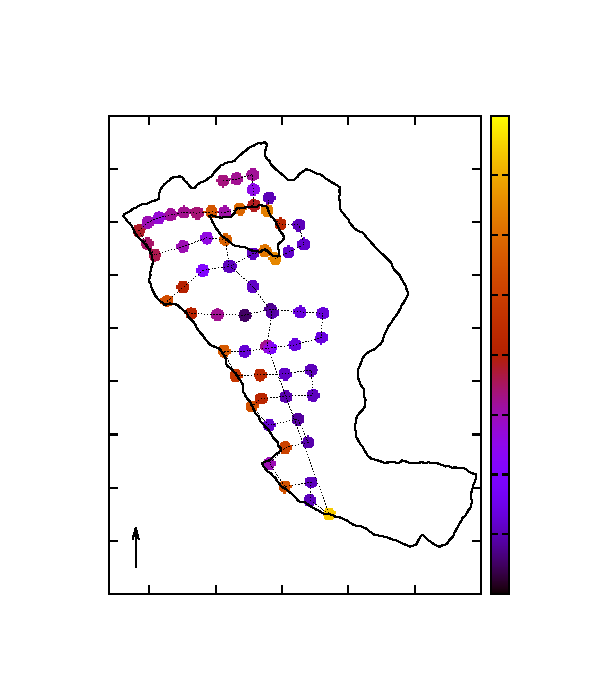
\includegraphics{tiefe}}%
    \gplfronttext
  \end{picture}%
\endgroup
}
	% GNUPLOT: LaTeX picture with Postscript
\begingroup
  \makeatletter
  \providecommand\color[2][]{%
    \GenericError{(gnuplot) \space\space\space\@spaces}{%
      Package color not loaded in conjunction with
      terminal option `colourtext'%
    }{See the gnuplot documentation for explanation.%
    }{Either use 'blacktext' in gnuplot or load the package
      color.sty in LaTeX.}%
    \renewcommand\color[2][]{}%
  }%
  \providecommand\includegraphics[2][]{%
    \GenericError{(gnuplot) \space\space\space\@spaces}{%
      Package graphicx or graphics not loaded%
    }{See the gnuplot documentation for explanation.%
    }{The gnuplot epslatex terminal needs graphicx.sty or graphics.sty.}%
    \renewcommand\includegraphics[2][]{}%
  }%
  \providecommand\rotatebox[2]{#2}%
  \@ifundefined{ifGPcolor}{%
    \newif\ifGPcolor
    \GPcolortrue
  }{}%
  \@ifundefined{ifGPblacktext}{%
    \newif\ifGPblacktext
    \GPblacktexttrue
  }{}%
  % define a \g@addto@macro without @ in the name:
  \let\gplgaddtomacro\g@addto@macro
  % define empty templates for all commands taking text:
  \gdef\gplbacktext{}%
  \gdef\gplfronttext{}%
  \makeatother
  \ifGPblacktext
    % no textcolor at all
    \def\colorrgb#1{}%
    \def\colorgray#1{}%
  \else
    % gray or color?
    \ifGPcolor
      \def\colorrgb#1{\color[rgb]{#1}}%
      \def\colorgray#1{\color[gray]{#1}}%
      \expandafter\def\csname LTw\endcsname{\color{white}}%
      \expandafter\def\csname LTb\endcsname{\color{black}}%
      \expandafter\def\csname LTa\endcsname{\color{black}}%
      \expandafter\def\csname LT0\endcsname{\color[rgb]{1,0,0}}%
      \expandafter\def\csname LT1\endcsname{\color[rgb]{0,1,0}}%
      \expandafter\def\csname LT2\endcsname{\color[rgb]{0,0,1}}%
      \expandafter\def\csname LT3\endcsname{\color[rgb]{1,0,1}}%
      \expandafter\def\csname LT4\endcsname{\color[rgb]{0,1,1}}%
      \expandafter\def\csname LT5\endcsname{\color[rgb]{1,1,0}}%
      \expandafter\def\csname LT6\endcsname{\color[rgb]{0,0,0}}%
      \expandafter\def\csname LT7\endcsname{\color[rgb]{1,0.3,0}}%
      \expandafter\def\csname LT8\endcsname{\color[rgb]{0.5,0.5,0.5}}%
    \else
      % gray
      \def\colorrgb#1{\color{black}}%
      \def\colorgray#1{\color[gray]{#1}}%
      \expandafter\def\csname LTw\endcsname{\color{white}}%
      \expandafter\def\csname LTb\endcsname{\color{black}}%
      \expandafter\def\csname LTa\endcsname{\color{black}}%
      \expandafter\def\csname LT0\endcsname{\color{black}}%
      \expandafter\def\csname LT1\endcsname{\color{black}}%
      \expandafter\def\csname LT2\endcsname{\color{black}}%
      \expandafter\def\csname LT3\endcsname{\color{black}}%
      \expandafter\def\csname LT4\endcsname{\color{black}}%
      \expandafter\def\csname LT5\endcsname{\color{black}}%
      \expandafter\def\csname LT6\endcsname{\color{black}}%
      \expandafter\def\csname LT7\endcsname{\color{black}}%
      \expandafter\def\csname LT8\endcsname{\color{black}}%
    \fi
  \fi
  \setlength{\unitlength}{0.0500bp}%
  \begin{picture}(7200.00,5040.00)%
    \gplgaddtomacro\gplbacktext{%
      \csname LTb\endcsname%
      \put(2503,1601){\makebox(0,0)[l]{\strut{}N}}%
    }%
    \gplgaddtomacro\gplfronttext{%
      \csname LTb\endcsname%
      \put(3945,1259){\makebox(0,0)[r]{\strut{}max. Tiefe}}%
      \csname LTb\endcsname%
      \put(2400,800){\makebox(0,0){\strut{}-400}}%
      \csname LTb\endcsname%
      \put(2743,800){\makebox(0,0){\strut{}-200}}%
      \csname LTb\endcsname%
      \put(3086,800){\makebox(0,0){\strut{} 0}}%
      \csname LTb\endcsname%
      \put(3429,800){\makebox(0,0){\strut{} 200}}%
      \csname LTb\endcsname%
      \put(3771,800){\makebox(0,0){\strut{} 400}}%
      \csname LTb\endcsname%
      \put(4114,800){\makebox(0,0){\strut{} 600}}%
      \csname LTb\endcsname%
      \put(4457,800){\makebox(0,0){\strut{} 800}}%
      \csname LTb\endcsname%
      \put(4800,800){\makebox(0,0){\strut{} 1000}}%
      \put(3600,470){\makebox(0,0){\strut{}$x$ [m]}}%
      \csname LTb\endcsname%
      \put(2228,1086){\makebox(0,0)[r]{\strut{}-1600}}%
      \csname LTb\endcsname%
      \put(2228,1429){\makebox(0,0)[r]{\strut{}-1400}}%
      \csname LTb\endcsname%
      \put(2228,1773){\makebox(0,0)[r]{\strut{}-1200}}%
      \csname LTb\endcsname%
      \put(2228,2116){\makebox(0,0)[r]{\strut{}-1000}}%
      \csname LTb\endcsname%
      \put(2228,2459){\makebox(0,0)[r]{\strut{}-800}}%
      \csname LTb\endcsname%
      \put(2228,2801){\makebox(0,0)[r]{\strut{}-600}}%
      \csname LTb\endcsname%
      \put(2228,3144){\makebox(0,0)[r]{\strut{}-400}}%
      \csname LTb\endcsname%
      \put(2228,3487){\makebox(0,0)[r]{\strut{}-200}}%
      \csname LTb\endcsname%
      \put(2228,3831){\makebox(0,0)[r]{\strut{} 0}}%
      \csname LTb\endcsname%
      \put(2228,4174){\makebox(0,0)[r]{\strut{} 200}}%
      \put(1502,2630){\rotatebox{-270}{\makebox(0,0){\strut{}$y$ [m]}}}%
      \put(5112,1086){\makebox(0,0)[l]{\strut{}-8}}%
      \put(5112,1472){\makebox(0,0)[l]{\strut{}-7}}%
      \put(5112,1858){\makebox(0,0)[l]{\strut{}-6}}%
      \put(5112,2244){\makebox(0,0)[l]{\strut{}-5}}%
      \put(5112,2630){\makebox(0,0)[l]{\strut{}-4}}%
      \put(5112,3016){\makebox(0,0)[l]{\strut{}-3}}%
      \put(5112,3402){\makebox(0,0)[l]{\strut{}-2}}%
      \put(5112,3788){\makebox(0,0)[l]{\strut{}-1}}%
      \put(5112,4174){\makebox(0,0)[l]{\strut{} 0}}%
      \put(5442,2630){\rotatebox{-270}{\makebox(0,0){\strut{}$z$ [m]}}}%
    }%
    \gplbacktext
    \put(0,0){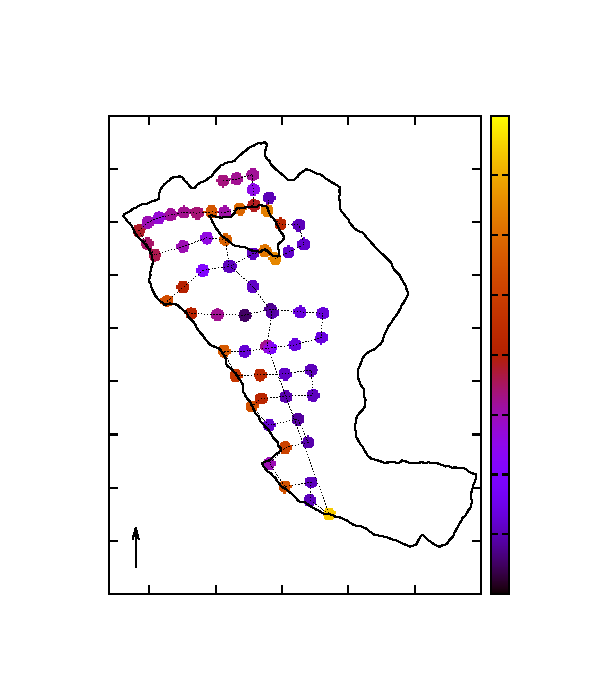
\includegraphics{tiefe}}%
    \gplfronttext
  \end{picture}%
\endgroup

	\caption{Messpunkte auf dem Northeimer See.}
	\label{fig:GPSNort}
\end{figure}

\subsection{Druck \& Tiefe}
\label{sec:ausdruck}
Laut Datenblatt und, wie im Kapitel \ref{sec:durchdruck} beschrieben, sollte der Spannungsverlauf der Druckmessbrücke linear mit dem Druck steigen und pro Bar ein Volt hinzubekommen.
Allerdings bemerkten wir schon während der Messung, dass die vom Datenlogger angezeigten Werte nicht ganz mit den von uns vorgenommenen Markierungen am Kabel im 1m Abstand übereinzustimmen schienen.
So ließen wir die Sensoren laut Kabel bis in eine Tiefe von ca. 7.5m hinab.
Allerdings ging die tiefste Messung laut aufgezeichneten Werten unter dieser Voraussetzung nur bis in eine Tiefe von ca. 6.8m.
Da jedoch eine 8m Wassersäule schon einen beachtlichen Druck ausübt, konnten wir keine Referenzmessung zur Eichung machen, so dass wir uns entschlossen haben, einen linearen Korrekturfaktor von 1.1 einzuführen, um dem jede vermeintliche Tiefe gestreckt wird.
Dieser Faktor ergibt sich aus den in Northeim gemessenen Tiefen und Druckdaten.
Unter dieser Annahme erhielten wir Werte, die mit den Beobachtungen übereinstimmten.
Die Linearität der Korrektur scheint in sofern angebracht, als dass wir uns bei vielen Messungen Mühe gegeben haben, die Sonde von Hand möglichst gleichmäßig herabzulassen.
Die aufgenommenen Druckkurven waren auch annähernd linear.

In Abbildung \ref{fig:tiefeGoe} ist die maximale Tiefe der einzelnen Messdaten an den jeweiligen Messpunkten dargestellt.
Man erkennt, dass der See am nördlichen Ende scheinbar mit etwa 2.2 Meter am tiefsten ist und nach Süden leicht flacher wird.
Für den Northeimer See ist es nicht sinnvoll, eine solche Karte zu erstellen, da die Sonde nur in Ufernähe Bodenkontakt hatte.
An den anderen Punkten war es tiefer als unser Kabel hergab, also tiefer als 7 Meter.

\begin{figure}[!htb]
	\centering
	% GNUPLOT: LaTeX picture with Postscript
\begingroup
  \makeatletter
  \providecommand\color[2][]{%
    \GenericError{(gnuplot) \space\space\space\@spaces}{%
      Package color not loaded in conjunction with
      terminal option `colourtext'%
    }{See the gnuplot documentation for explanation.%
    }{Either use 'blacktext' in gnuplot or load the package
      color.sty in LaTeX.}%
    \renewcommand\color[2][]{}%
  }%
  \providecommand\includegraphics[2][]{%
    \GenericError{(gnuplot) \space\space\space\@spaces}{%
      Package graphicx or graphics not loaded%
    }{See the gnuplot documentation for explanation.%
    }{The gnuplot epslatex terminal needs graphicx.sty or graphics.sty.}%
    \renewcommand\includegraphics[2][]{}%
  }%
  \providecommand\rotatebox[2]{#2}%
  \@ifundefined{ifGPcolor}{%
    \newif\ifGPcolor
    \GPcolortrue
  }{}%
  \@ifundefined{ifGPblacktext}{%
    \newif\ifGPblacktext
    \GPblacktexttrue
  }{}%
  % define a \g@addto@macro without @ in the name:
  \let\gplgaddtomacro\g@addto@macro
  % define empty templates for all commands taking text:
  \gdef\gplbacktext{}%
  \gdef\gplfronttext{}%
  \makeatother
  \ifGPblacktext
    % no textcolor at all
    \def\colorrgb#1{}%
    \def\colorgray#1{}%
  \else
    % gray or color?
    \ifGPcolor
      \def\colorrgb#1{\color[rgb]{#1}}%
      \def\colorgray#1{\color[gray]{#1}}%
      \expandafter\def\csname LTw\endcsname{\color{white}}%
      \expandafter\def\csname LTb\endcsname{\color{black}}%
      \expandafter\def\csname LTa\endcsname{\color{black}}%
      \expandafter\def\csname LT0\endcsname{\color[rgb]{1,0,0}}%
      \expandafter\def\csname LT1\endcsname{\color[rgb]{0,1,0}}%
      \expandafter\def\csname LT2\endcsname{\color[rgb]{0,0,1}}%
      \expandafter\def\csname LT3\endcsname{\color[rgb]{1,0,1}}%
      \expandafter\def\csname LT4\endcsname{\color[rgb]{0,1,1}}%
      \expandafter\def\csname LT5\endcsname{\color[rgb]{1,1,0}}%
      \expandafter\def\csname LT6\endcsname{\color[rgb]{0,0,0}}%
      \expandafter\def\csname LT7\endcsname{\color[rgb]{1,0.3,0}}%
      \expandafter\def\csname LT8\endcsname{\color[rgb]{0.5,0.5,0.5}}%
    \else
      % gray
      \def\colorrgb#1{\color{black}}%
      \def\colorgray#1{\color[gray]{#1}}%
      \expandafter\def\csname LTw\endcsname{\color{white}}%
      \expandafter\def\csname LTb\endcsname{\color{black}}%
      \expandafter\def\csname LTa\endcsname{\color{black}}%
      \expandafter\def\csname LT0\endcsname{\color{black}}%
      \expandafter\def\csname LT1\endcsname{\color{black}}%
      \expandafter\def\csname LT2\endcsname{\color{black}}%
      \expandafter\def\csname LT3\endcsname{\color{black}}%
      \expandafter\def\csname LT4\endcsname{\color{black}}%
      \expandafter\def\csname LT5\endcsname{\color{black}}%
      \expandafter\def\csname LT6\endcsname{\color{black}}%
      \expandafter\def\csname LT7\endcsname{\color{black}}%
      \expandafter\def\csname LT8\endcsname{\color{black}}%
    \fi
  \fi
  \setlength{\unitlength}{0.0500bp}%
  \begin{picture}(7200.00,5040.00)%
    \gplgaddtomacro\gplbacktext{%
      \csname LTb\endcsname%
      \put(1513,1738){\makebox(0,0)[l]{\strut{}N}}%
    }%
    \gplgaddtomacro\gplfronttext{%
      \csname LTb\endcsname%
      \put(5175,1660){\makebox(0,0)[r]{\strut{}max. Tiefe}}%
      \csname LTb\endcsname%
      \put(1456,1201){\makebox(0,0){\strut{}-100}}%
      \put(2028,1201){\makebox(0,0){\strut{} 0}}%
      \put(2600,1201){\makebox(0,0){\strut{} 100}}%
      \put(3172,1201){\makebox(0,0){\strut{} 200}}%
      \put(3742,1201){\makebox(0,0){\strut{} 300}}%
      \put(4314,1201){\makebox(0,0){\strut{} 400}}%
      \put(4886,1201){\makebox(0,0){\strut{} 500}}%
      \put(5458,1201){\makebox(0,0){\strut{} 600}}%
      \put(6030,1201){\makebox(0,0){\strut{} 700}}%
      \put(3600,871){\makebox(0,0){\strut{}$x$ [m]}}%
      \put(998,1487){\makebox(0,0)[r]{\strut{}-100}}%
      \put(998,1773){\makebox(0,0)[r]{\strut{}-50}}%
      \put(998,2059){\makebox(0,0)[r]{\strut{} 0}}%
      \put(998,2345){\makebox(0,0)[r]{\strut{} 50}}%
      \put(998,2630){\makebox(0,0)[r]{\strut{} 100}}%
      \put(998,2915){\makebox(0,0)[r]{\strut{} 150}}%
      \put(998,3201){\makebox(0,0)[r]{\strut{} 200}}%
      \put(998,3487){\makebox(0,0)[r]{\strut{} 250}}%
      \put(998,3773){\makebox(0,0)[r]{\strut{} 300}}%
      \put(404,2630){\rotatebox{-270}{\makebox(0,0){\strut{}$y$ [m]}}}%
      \put(6527,1487){\makebox(0,0)[l]{\strut{}-2.2}}%
      \put(6527,1813){\makebox(0,0)[l]{\strut{}-2}}%
      \put(6527,2140){\makebox(0,0)[l]{\strut{}-1.8}}%
      \put(6527,2466){\makebox(0,0)[l]{\strut{}-1.6}}%
      \put(6527,2793){\makebox(0,0)[l]{\strut{}-1.4}}%
      \put(6527,3119){\makebox(0,0)[l]{\strut{}-1.2}}%
      \put(6527,3446){\makebox(0,0)[l]{\strut{}-1}}%
      \put(6527,3772){\makebox(0,0)[l]{\strut{}-0.8}}%
      \put(7121,2630){\rotatebox{-270}{\makebox(0,0){\strut{}$z$ [m]}}}%
    }%
    \gplbacktext
    \put(0,0){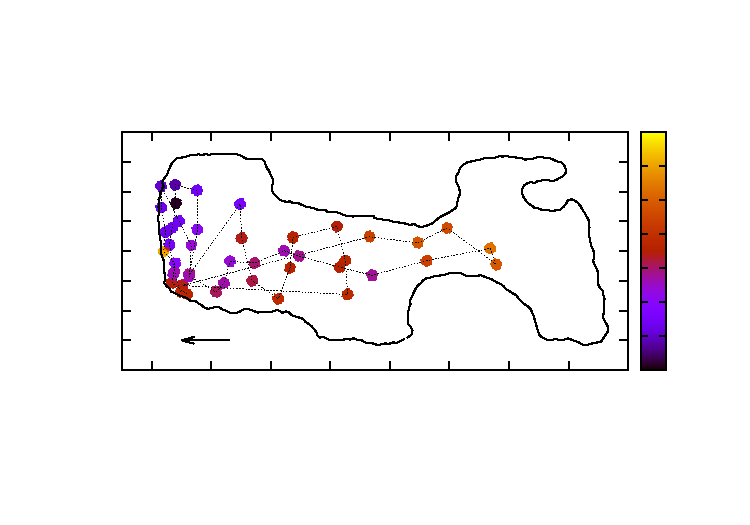
\includegraphics{tiefeGoe}}%
    \gplfronttext
  \end{picture}%
\endgroup

	\caption{Göttinger Kiessee: Tiefe.}
	\label{fig:tiefeGoe}
\end{figure}

Die Druckkurven besaßen eine Breite (und in sofern ein Fehlerintervall) von ca. 15cm.
Für die Temperaturwerte der Northeimer Messung mussten wir die Daten bearbeiten.
Da wir aufgrund der springenden Temperatur die Daten in 40er Blöcke unterteilt haben, nahmen wir von den Tiefendaten den Mittelwert.


\subsection{Temperatur}
\subsubsection{Göttingen}
In Abb. \ref{fig:temp_goe} sind alle von uns aufgenommenen Temperaturen bis $40\,\si{\celsius}$ aufgetragen.
Darüber\-hinaus waren noch einige Werte bei bis zu $140\,\si{\celsius}$, welche jedoch augenscheinlich durch einen Wackelkontakt in der Stromversorgung zustande kamen.
Ebenfalls ist dort ein linearer Fit über die Werte, welche im Wasser aufgenommen wurden und sich unterhalb von $24\,\si{\celsius}$ befinden.
Von diesen nehmen wir nämlich an, dass sie richtig sind und dort der Temperaturwiderstand mit der richtigen Spannung von $3.3\,$V betrieben wird.
Die Gerade hat die Form $T(z)=(21.2\pm 0.7)\si{\celsius}-(0.43\pm 0.05)\si{\celsius\per\meter}\cdot z$.
An ihr kann man den allgemeinen Trend erkennen, dass es pro Meter etwa $0.4\si{\celsius}$ bis  $0.5\si{\celsius}$  kälter wird.
Die Messwerte schwanken jedoch um diese Gerade um bis zu $2\si{\celsius}$.
Sie stammen aber auch von mehreren Messreihen, also von unterschiedlichen Orten und zu verschiedenen Zeiten.
So sind die angegebenen Fehler keine Fehlerwerte aus einem linearen Fit, sondern resultieren aus verschiedenen Einschränkungen des akzeptierten Wertebereichs, denn die Korrelation der Daten ist auf Grund der starken Streuung nicht besonders gut.
Eine genauere Auswertung ist auf Grund der wenigen brauchbaren Messreihen und der vergleichsweise geringen Zeitspanne nicht möglich.\\
In den Abbildung \ref{fig:tempGoeBsp1} ist noch einmal zu sehen, dass die Temperatur sich Zeitlich extremstark ändert.
Diese Daten sind nicht auszuwerten, da sich der See in der angegebenen Zeit nicht in der Temperatur verdoppelt hat.
Es ist in diesen Daten kein Muster zu erkennen, dass sich eindeutig einem bestimmten Fehler zuordnen lässt, wie im nächsten Kapitel es der Fall war.\\
In der Abbildung \ref{fig:tempGoeBsp2} ist nocheinmal der gleiche Datensatz Datensatz von 15:14 Uhr, wie in der Abbildung \ref{fig:tempGoeBsp1} zu sehen.
Dieser Plot zeigt, dass sich die zwei linien, die man gegen die Tiefe aufgetragen erkennent, durch einen Sprung zustanden kommen, der gegen die Zeit ausgetragen zu erkennen ist.
Dieser Sprung verdeutlicht den Wackelkontackt, der oben bereits angemerkt wurde.
Somit sind auch diese Daten nicht auswertbar, da man nicht sagen kann welche von beiden die richtige Linie für die Temperatur im See ist.
Hierzu hätte eine genau Messung mit einem geeichten Messgerät durchgeführt werden sollen.\\
Die Abbildung \ref{fig:tempSchlamm} zeigt einen weiteren Temperaturverlauf gegen die Tiefe aufgetragen.
In diesem Plot ergeben sich zwei Linien, die einen stetigen Übergang in einer bestimtem Tiefe besitzen.
Bei dieser Messung traf die Sonden auf dem Boden auf und sammelte Schlamm an, welcher wieder nach oben befördert wurde.
Die Temperatur verläuft von oben nach unten, da der Schlamm unten im See deutlich kühler ist, als das umgebene Wasser.
Auch diese Daten sind nicht auszuwerten, da die Schlammtemperatur aus fast allen Datensätzen gefilter werden muss.

\begin{figure}[h]
\centering
% GNUPLOT: LaTeX picture with Postscript
\begingroup
  \makeatletter
  \providecommand\color[2][]{%
    \GenericError{(gnuplot) \space\space\space\@spaces}{%
      Package color not loaded in conjunction with
      terminal option `colourtext'%
    }{See the gnuplot documentation for explanation.%
    }{Either use 'blacktext' in gnuplot or load the package
      color.sty in LaTeX.}%
    \renewcommand\color[2][]{}%
  }%
  \providecommand\includegraphics[2][]{%
    \GenericError{(gnuplot) \space\space\space\@spaces}{%
      Package graphicx or graphics not loaded%
    }{See the gnuplot documentation for explanation.%
    }{The gnuplot epslatex terminal needs graphicx.sty or graphics.sty.}%
    \renewcommand\includegraphics[2][]{}%
  }%
  \providecommand\rotatebox[2]{#2}%
  \@ifundefined{ifGPcolor}{%
    \newif\ifGPcolor
    \GPcolortrue
  }{}%
  \@ifundefined{ifGPblacktext}{%
    \newif\ifGPblacktext
    \GPblacktexttrue
  }{}%
  % define a \g@addto@macro without @ in the name:
  \let\gplgaddtomacro\g@addto@macro
  % define empty templates for all commands taking text:
  \gdef\gplbacktext{}%
  \gdef\gplfronttext{}%
  \makeatother
  \ifGPblacktext
    % no textcolor at all
    \def\colorrgb#1{}%
    \def\colorgray#1{}%
  \else
    % gray or color?
    \ifGPcolor
      \def\colorrgb#1{\color[rgb]{#1}}%
      \def\colorgray#1{\color[gray]{#1}}%
      \expandafter\def\csname LTw\endcsname{\color{white}}%
      \expandafter\def\csname LTb\endcsname{\color{black}}%
      \expandafter\def\csname LTa\endcsname{\color{black}}%
      \expandafter\def\csname LT0\endcsname{\color[rgb]{1,0,0}}%
      \expandafter\def\csname LT1\endcsname{\color[rgb]{0,1,0}}%
      \expandafter\def\csname LT2\endcsname{\color[rgb]{0,0,1}}%
      \expandafter\def\csname LT3\endcsname{\color[rgb]{1,0,1}}%
      \expandafter\def\csname LT4\endcsname{\color[rgb]{0,1,1}}%
      \expandafter\def\csname LT5\endcsname{\color[rgb]{1,1,0}}%
      \expandafter\def\csname LT6\endcsname{\color[rgb]{0,0,0}}%
      \expandafter\def\csname LT7\endcsname{\color[rgb]{1,0.3,0}}%
      \expandafter\def\csname LT8\endcsname{\color[rgb]{0.5,0.5,0.5}}%
    \else
      % gray
      \def\colorrgb#1{\color{black}}%
      \def\colorgray#1{\color[gray]{#1}}%
      \expandafter\def\csname LTw\endcsname{\color{white}}%
      \expandafter\def\csname LTb\endcsname{\color{black}}%
      \expandafter\def\csname LTa\endcsname{\color{black}}%
      \expandafter\def\csname LT0\endcsname{\color{black}}%
      \expandafter\def\csname LT1\endcsname{\color{black}}%
      \expandafter\def\csname LT2\endcsname{\color{black}}%
      \expandafter\def\csname LT3\endcsname{\color{black}}%
      \expandafter\def\csname LT4\endcsname{\color{black}}%
      \expandafter\def\csname LT5\endcsname{\color{black}}%
      \expandafter\def\csname LT6\endcsname{\color{black}}%
      \expandafter\def\csname LT7\endcsname{\color{black}}%
      \expandafter\def\csname LT8\endcsname{\color{black}}%
    \fi
  \fi
  \setlength{\unitlength}{0.0500bp}%
  \begin{picture}(7200.00,5040.00)%
    \gplgaddtomacro\gplbacktext{%
      \csname LTb\endcsname%
      \put(814,704){\makebox(0,0)[r]{\strut{} 15}}%
      \put(814,1518){\makebox(0,0)[r]{\strut{} 20}}%
      \put(814,2332){\makebox(0,0)[r]{\strut{} 25}}%
      \put(814,3147){\makebox(0,0)[r]{\strut{} 30}}%
      \put(814,3961){\makebox(0,0)[r]{\strut{} 35}}%
      \put(814,4775){\makebox(0,0)[r]{\strut{} 40}}%
      \put(1380,484){\makebox(0,0){\strut{} 0}}%
      \put(2464,484){\makebox(0,0){\strut{} 0.5}}%
      \put(3549,484){\makebox(0,0){\strut{} 1}}%
      \put(4634,484){\makebox(0,0){\strut{} 1.5}}%
      \put(5718,484){\makebox(0,0){\strut{} 2}}%
      \put(6803,484){\makebox(0,0){\strut{} 2.5}}%
      \put(176,2739){\rotatebox{-270}{\makebox(0,0){\strut{}$T\, [\si{\celsius}]$}}}%
      \put(3874,154){\makebox(0,0){\strut{}$z$ [m]}}%
    }%
    \gplgaddtomacro\gplfronttext{%
      \csname LTb\endcsname%
      \put(5816,1097){\makebox(0,0)[r]{\strut{}Messwerte (ohne Ausreißer)}}%
      \csname LTb\endcsname%
      \put(5816,877){\makebox(0,0)[r]{\strut{}Approximation}}%
    }%
    \gplbacktext
    \put(0,0){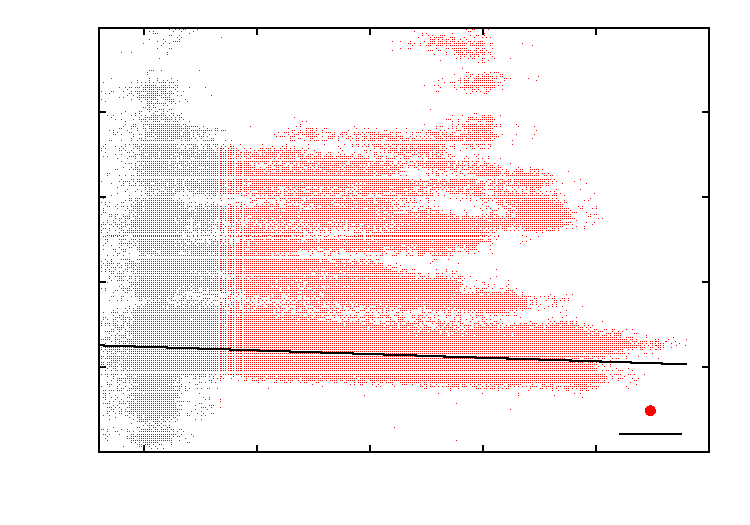
\includegraphics{temp_goe}}%
    \gplfronttext
  \end{picture}%
\endgroup

\caption{Temperaturverlauf am Göttinger Kiessee mit fast allen aufgenommenen Werten. Einige Werte, welche offensichtlich durch Wackelkontakte zu Stande kommen (bis zu $140^\circ$C) wurden zwecks Übersichtlichkeit ausgeblendet.}
\label{fig:temp_goe}
\end{figure}

\begin{figure}[!h]
	\centering
	\subfigure[Temperaturverlauf von zwei ausgesuchten Datensätzen in Göttingen gegen Tiefe. \label{fig:tempGoeBsp1}]
   {\resizebox{0.49\linewidth}{!}{% GNUPLOT: LaTeX picture with Postscript
\begingroup
  \makeatletter
  \providecommand\color[2][]{%
    \GenericError{(gnuplot) \space\space\space\@spaces}{%
      Package color not loaded in conjunction with
      terminal option `colourtext'%
    }{See the gnuplot documentation for explanation.%
    }{Either use 'blacktext' in gnuplot or load the package
      color.sty in LaTeX.}%
    \renewcommand\color[2][]{}%
  }%
  \providecommand\includegraphics[2][]{%
    \GenericError{(gnuplot) \space\space\space\@spaces}{%
      Package graphicx or graphics not loaded%
    }{See the gnuplot documentation for explanation.%
    }{The gnuplot epslatex terminal needs graphicx.sty or graphics.sty.}%
    \renewcommand\includegraphics[2][]{}%
  }%
  \providecommand\rotatebox[2]{#2}%
  \@ifundefined{ifGPcolor}{%
    \newif\ifGPcolor
    \GPcolortrue
  }{}%
  \@ifundefined{ifGPblacktext}{%
    \newif\ifGPblacktext
    \GPblacktexttrue
  }{}%
  % define a \g@addto@macro without @ in the name:
  \let\gplgaddtomacro\g@addto@macro
  % define empty templates for all commands taking text:
  \gdef\gplbacktext{}%
  \gdef\gplfronttext{}%
  \makeatother
  \ifGPblacktext
    % no textcolor at all
    \def\colorrgb#1{}%
    \def\colorgray#1{}%
  \else
    % gray or color?
    \ifGPcolor
      \def\colorrgb#1{\color[rgb]{#1}}%
      \def\colorgray#1{\color[gray]{#1}}%
      \expandafter\def\csname LTw\endcsname{\color{white}}%
      \expandafter\def\csname LTb\endcsname{\color{black}}%
      \expandafter\def\csname LTa\endcsname{\color{black}}%
      \expandafter\def\csname LT0\endcsname{\color[rgb]{1,0,0}}%
      \expandafter\def\csname LT1\endcsname{\color[rgb]{0,1,0}}%
      \expandafter\def\csname LT2\endcsname{\color[rgb]{0,0,1}}%
      \expandafter\def\csname LT3\endcsname{\color[rgb]{1,0,1}}%
      \expandafter\def\csname LT4\endcsname{\color[rgb]{0,1,1}}%
      \expandafter\def\csname LT5\endcsname{\color[rgb]{1,1,0}}%
      \expandafter\def\csname LT6\endcsname{\color[rgb]{0,0,0}}%
      \expandafter\def\csname LT7\endcsname{\color[rgb]{1,0.3,0}}%
      \expandafter\def\csname LT8\endcsname{\color[rgb]{0.5,0.5,0.5}}%
    \else
      % gray
      \def\colorrgb#1{\color{black}}%
      \def\colorgray#1{\color[gray]{#1}}%
      \expandafter\def\csname LTw\endcsname{\color{white}}%
      \expandafter\def\csname LTb\endcsname{\color{black}}%
      \expandafter\def\csname LTa\endcsname{\color{black}}%
      \expandafter\def\csname LT0\endcsname{\color{black}}%
      \expandafter\def\csname LT1\endcsname{\color{black}}%
      \expandafter\def\csname LT2\endcsname{\color{black}}%
      \expandafter\def\csname LT3\endcsname{\color{black}}%
      \expandafter\def\csname LT4\endcsname{\color{black}}%
      \expandafter\def\csname LT5\endcsname{\color{black}}%
      \expandafter\def\csname LT6\endcsname{\color{black}}%
      \expandafter\def\csname LT7\endcsname{\color{black}}%
      \expandafter\def\csname LT8\endcsname{\color{black}}%
    \fi
  \fi
  \setlength{\unitlength}{0.0500bp}%
  \begin{picture}(7200.00,5040.00)%
    \gplgaddtomacro\gplbacktext{%
      \csname LTb\endcsname%
      \put(814,704){\makebox(0,0)[r]{\strut{} 15}}%
      \put(814,1518){\makebox(0,0)[r]{\strut{} 20}}%
      \put(814,2332){\makebox(0,0)[r]{\strut{} 25}}%
      \put(814,3147){\makebox(0,0)[r]{\strut{} 30}}%
      \put(814,3961){\makebox(0,0)[r]{\strut{} 35}}%
      \put(814,4775){\makebox(0,0)[r]{\strut{} 40}}%
      \put(946,484){\makebox(0,0){\strut{}-0.2}}%
      \put(1532,484){\makebox(0,0){\strut{} 0}}%
      \put(2117,484){\makebox(0,0){\strut{} 0.2}}%
      \put(2703,484){\makebox(0,0){\strut{} 0.4}}%
      \put(3289,484){\makebox(0,0){\strut{} 0.6}}%
      \put(3875,484){\makebox(0,0){\strut{} 0.8}}%
      \put(4460,484){\makebox(0,0){\strut{} 1}}%
      \put(5046,484){\makebox(0,0){\strut{} 1.2}}%
      \put(5632,484){\makebox(0,0){\strut{} 1.4}}%
      \put(6217,484){\makebox(0,0){\strut{} 1.6}}%
      \put(6803,484){\makebox(0,0){\strut{} 1.8}}%
      \put(176,2739){\rotatebox{-270}{\makebox(0,0){\strut{}$T\, [\si{\celsius}]$}}}%
      \put(3874,154){\makebox(0,0){\strut{}$z$ [m]}}%
    }%
    \gplgaddtomacro\gplfronttext{%
      \csname LTb\endcsname%
      \put(5816,4602){\makebox(0,0)[r]{\strut{}14:34 Uhr}}%
      \csname LTb\endcsname%
      \put(5816,4382){\makebox(0,0)[r]{\strut{}15:14 Uhr}}%
    }%
    \gplbacktext
    \put(0,0){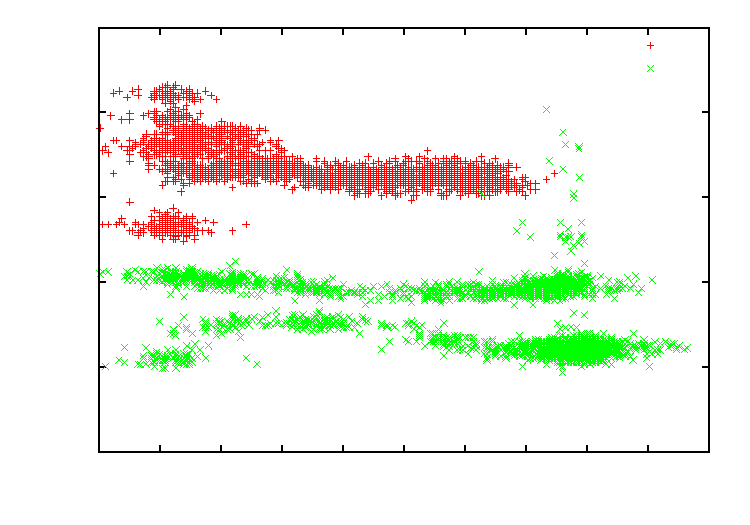
\includegraphics{temp_goe_bsp}}%
    \gplfronttext
  \end{picture}%
\endgroup
}}
   \hfill
   \subfigure[Temperaturverlauf von einer ausgewählten Messreihe in Göttingen gegen Zeit.\label{fig:tempGoeBsp2}]
   {\resizebox{.49\linewidth}{!}{% GNUPLOT: LaTeX picture with Postscript
\begingroup
  \makeatletter
  \providecommand\color[2][]{%
    \GenericError{(gnuplot) \space\space\space\@spaces}{%
      Package color not loaded in conjunction with
      terminal option `colourtext'%
    }{See the gnuplot documentation for explanation.%
    }{Either use 'blacktext' in gnuplot or load the package
      color.sty in LaTeX.}%
    \renewcommand\color[2][]{}%
  }%
  \providecommand\includegraphics[2][]{%
    \GenericError{(gnuplot) \space\space\space\@spaces}{%
      Package graphicx or graphics not loaded%
    }{See the gnuplot documentation for explanation.%
    }{The gnuplot epslatex terminal needs graphicx.sty or graphics.sty.}%
    \renewcommand\includegraphics[2][]{}%
  }%
  \providecommand\rotatebox[2]{#2}%
  \@ifundefined{ifGPcolor}{%
    \newif\ifGPcolor
    \GPcolortrue
  }{}%
  \@ifundefined{ifGPblacktext}{%
    \newif\ifGPblacktext
    \GPblacktexttrue
  }{}%
  % define a \g@addto@macro without @ in the name:
  \let\gplgaddtomacro\g@addto@macro
  % define empty templates for all commands taking text:
  \gdef\gplbacktext{}%
  \gdef\gplfronttext{}%
  \makeatother
  \ifGPblacktext
    % no textcolor at all
    \def\colorrgb#1{}%
    \def\colorgray#1{}%
  \else
    % gray or color?
    \ifGPcolor
      \def\colorrgb#1{\color[rgb]{#1}}%
      \def\colorgray#1{\color[gray]{#1}}%
      \expandafter\def\csname LTw\endcsname{\color{white}}%
      \expandafter\def\csname LTb\endcsname{\color{black}}%
      \expandafter\def\csname LTa\endcsname{\color{black}}%
      \expandafter\def\csname LT0\endcsname{\color[rgb]{1,0,0}}%
      \expandafter\def\csname LT1\endcsname{\color[rgb]{0,1,0}}%
      \expandafter\def\csname LT2\endcsname{\color[rgb]{0,0,1}}%
      \expandafter\def\csname LT3\endcsname{\color[rgb]{1,0,1}}%
      \expandafter\def\csname LT4\endcsname{\color[rgb]{0,1,1}}%
      \expandafter\def\csname LT5\endcsname{\color[rgb]{1,1,0}}%
      \expandafter\def\csname LT6\endcsname{\color[rgb]{0,0,0}}%
      \expandafter\def\csname LT7\endcsname{\color[rgb]{1,0.3,0}}%
      \expandafter\def\csname LT8\endcsname{\color[rgb]{0.5,0.5,0.5}}%
    \else
      % gray
      \def\colorrgb#1{\color{black}}%
      \def\colorgray#1{\color[gray]{#1}}%
      \expandafter\def\csname LTw\endcsname{\color{white}}%
      \expandafter\def\csname LTb\endcsname{\color{black}}%
      \expandafter\def\csname LTa\endcsname{\color{black}}%
      \expandafter\def\csname LT0\endcsname{\color{black}}%
      \expandafter\def\csname LT1\endcsname{\color{black}}%
      \expandafter\def\csname LT2\endcsname{\color{black}}%
      \expandafter\def\csname LT3\endcsname{\color{black}}%
      \expandafter\def\csname LT4\endcsname{\color{black}}%
      \expandafter\def\csname LT5\endcsname{\color{black}}%
      \expandafter\def\csname LT6\endcsname{\color{black}}%
      \expandafter\def\csname LT7\endcsname{\color{black}}%
      \expandafter\def\csname LT8\endcsname{\color{black}}%
    \fi
  \fi
  \setlength{\unitlength}{0.0500bp}%
  \begin{picture}(7200.00,5040.00)%
    \gplgaddtomacro\gplbacktext{%
      \csname LTb\endcsname%
      \put(814,704){\makebox(0,0)[r]{\strut{} 15}}%
      \put(814,1518){\makebox(0,0)[r]{\strut{} 20}}%
      \put(814,2332){\makebox(0,0)[r]{\strut{} 25}}%
      \put(814,3147){\makebox(0,0)[r]{\strut{} 30}}%
      \put(814,3961){\makebox(0,0)[r]{\strut{} 35}}%
      \put(814,4775){\makebox(0,0)[r]{\strut{} 40}}%
      \put(972,484){\makebox(0,0){\strut{} 0}}%
      \put(1620,484){\makebox(0,0){\strut{} 5}}%
      \put(2268,484){\makebox(0,0){\strut{} 10}}%
      \put(2916,484){\makebox(0,0){\strut{} 15}}%
      \put(3564,484){\makebox(0,0){\strut{} 20}}%
      \put(4211,484){\makebox(0,0){\strut{} 25}}%
      \put(4859,484){\makebox(0,0){\strut{} 30}}%
      \put(5507,484){\makebox(0,0){\strut{} 35}}%
      \put(6155,484){\makebox(0,0){\strut{} 40}}%
      \put(6803,484){\makebox(0,0){\strut{} 45}}%
      \put(176,2739){\rotatebox{-270}{\makebox(0,0){\strut{}$T\, [\si{\celsius}]$}}}%
      \put(3874,154){\makebox(0,0){\strut{}Zeit t[s]}}%
    }%
    \gplgaddtomacro\gplfronttext{%
      \csname LTb\endcsname%
      \put(5816,4602){\makebox(0,0)[r]{\strut{}15:14 Uhr}}%
    }%
    \gplbacktext
    \put(0,0){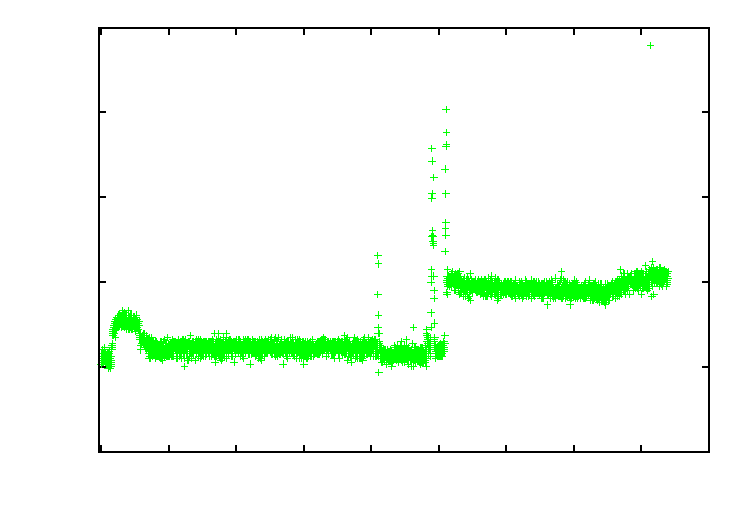
\includegraphics{temp_goe_bsp2}}%
    \gplfronttext
  \end{picture}%
\endgroup
}}
	\caption{Aus der Messreihe in Göttingen wurden zwei beispielhafte Verläufe der Temperatur gegen Zeit und Tiefe aufgetragen.}
	\label{fig:tempGoeBsp}
\end{figure}

\begin{figure}[!h]
	\centering
	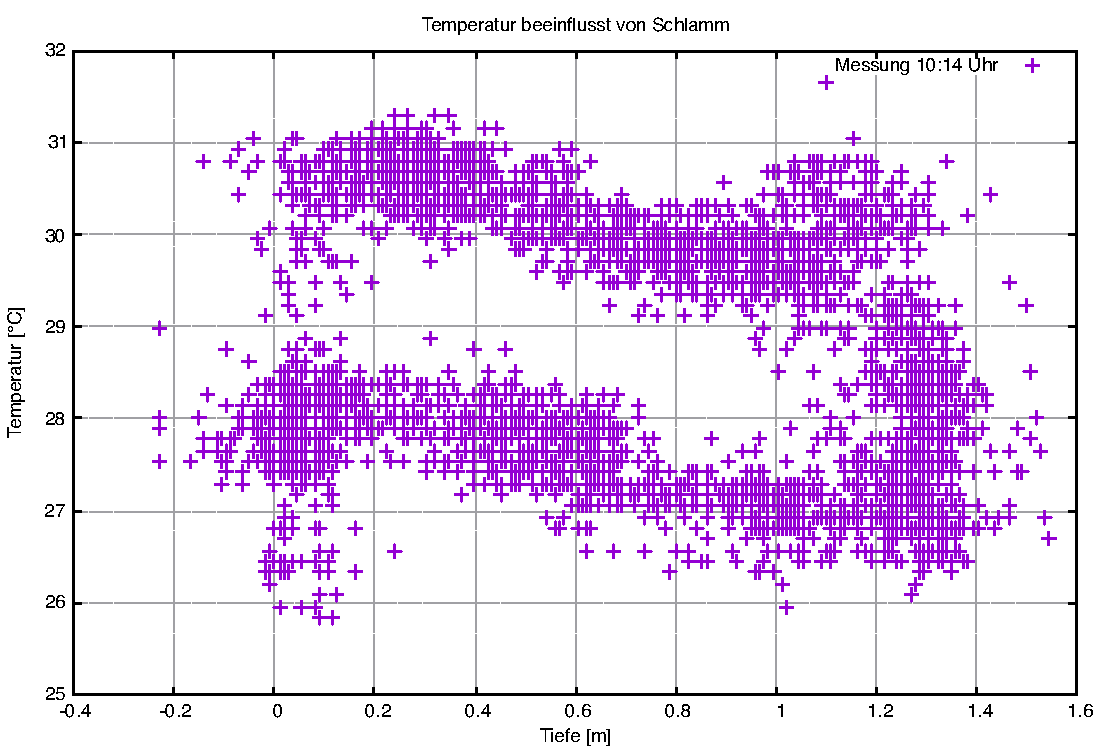
\includegraphics[width=0.8\linewidth]{TempSchlamm}
	\caption{Bei der Messung in Göttingen wird der Einfluss von Schlamm auf dem Temperatursensor gezeigt. Die obere Kurve entstand beim hinunterlassen, die untere beim hochziehen. Es ist zu dem der Stätige Übergang zwischen den beiden Linien bei fester Tiefe zu sehen.}
	\label{fig:tempSchlamm}
\end{figure}



\subsubsection{Northeim}
\label{sec:austempnortheim}
\begin{figure}[!htb]
	\centering
	\subfigure[Rohdaten der Temperaturmessung. \label{fig:temp_nor_Roh}]
	{\resizebox{0.39\textwidth}{!}{% GNUPLOT: LaTeX picture with Postscript
\begingroup
  \makeatletter
  \providecommand\color[2][]{%
    \GenericError{(gnuplot) \space\space\space\@spaces}{%
      Package color not loaded in conjunction with
      terminal option `colourtext'%
    }{See the gnuplot documentation for explanation.%
    }{Either use 'blacktext' in gnuplot or load the package
      color.sty in LaTeX.}%
    \renewcommand\color[2][]{}%
  }%
  \providecommand\includegraphics[2][]{%
    \GenericError{(gnuplot) \space\space\space\@spaces}{%
      Package graphicx or graphics not loaded%
    }{See the gnuplot documentation for explanation.%
    }{The gnuplot epslatex terminal needs graphicx.sty or graphics.sty.}%
    \renewcommand\includegraphics[2][]{}%
  }%
  \providecommand\rotatebox[2]{#2}%
  \@ifundefined{ifGPcolor}{%
    \newif\ifGPcolor
    \GPcolortrue
  }{}%
  \@ifundefined{ifGPblacktext}{%
    \newif\ifGPblacktext
    \GPblacktexttrue
  }{}%
  % define a \g@addto@macro without @ in the name:
  \let\gplgaddtomacro\g@addto@macro
  % define empty templates for all commands taking text:
  \gdef\gplbacktext{}%
  \gdef\gplfronttext{}%
  \makeatother
  \ifGPblacktext
    % no textcolor at all
    \def\colorrgb#1{}%
    \def\colorgray#1{}%
  \else
    % gray or color?
    \ifGPcolor
      \def\colorrgb#1{\color[rgb]{#1}}%
      \def\colorgray#1{\color[gray]{#1}}%
      \expandafter\def\csname LTw\endcsname{\color{white}}%
      \expandafter\def\csname LTb\endcsname{\color{black}}%
      \expandafter\def\csname LTa\endcsname{\color{black}}%
      \expandafter\def\csname LT0\endcsname{\color[rgb]{1,0,0}}%
      \expandafter\def\csname LT1\endcsname{\color[rgb]{0,1,0}}%
      \expandafter\def\csname LT2\endcsname{\color[rgb]{0,0,1}}%
      \expandafter\def\csname LT3\endcsname{\color[rgb]{1,0,1}}%
      \expandafter\def\csname LT4\endcsname{\color[rgb]{0,1,1}}%
      \expandafter\def\csname LT5\endcsname{\color[rgb]{1,1,0}}%
      \expandafter\def\csname LT6\endcsname{\color[rgb]{0,0,0}}%
      \expandafter\def\csname LT7\endcsname{\color[rgb]{1,0.3,0}}%
      \expandafter\def\csname LT8\endcsname{\color[rgb]{0.5,0.5,0.5}}%
    \else
      % gray
      \def\colorrgb#1{\color{black}}%
      \def\colorgray#1{\color[gray]{#1}}%
      \expandafter\def\csname LTw\endcsname{\color{white}}%
      \expandafter\def\csname LTb\endcsname{\color{black}}%
      \expandafter\def\csname LTa\endcsname{\color{black}}%
      \expandafter\def\csname LT0\endcsname{\color{black}}%
      \expandafter\def\csname LT1\endcsname{\color{black}}%
      \expandafter\def\csname LT2\endcsname{\color{black}}%
      \expandafter\def\csname LT3\endcsname{\color{black}}%
      \expandafter\def\csname LT4\endcsname{\color{black}}%
      \expandafter\def\csname LT5\endcsname{\color{black}}%
      \expandafter\def\csname LT6\endcsname{\color{black}}%
      \expandafter\def\csname LT7\endcsname{\color{black}}%
      \expandafter\def\csname LT8\endcsname{\color{black}}%
    \fi
  \fi
  \setlength{\unitlength}{0.0500bp}%
  \begin{picture}(7200.00,5040.00)%
    \gplgaddtomacro\gplbacktext{%
      \csname LTb\endcsname%
      \put(814,704){\makebox(0,0)[r]{\strut{} 10}}%
      \put(814,1518){\makebox(0,0)[r]{\strut{} 15}}%
      \put(814,2332){\makebox(0,0)[r]{\strut{} 20}}%
      \put(814,3147){\makebox(0,0)[r]{\strut{} 25}}%
      \put(814,3961){\makebox(0,0)[r]{\strut{} 30}}%
      \put(814,4775){\makebox(0,0)[r]{\strut{} 35}}%
      \put(1098,484){\makebox(0,0){\strut{} 0}}%
      \put(1859,484){\makebox(0,0){\strut{} 1}}%
      \put(2619,484){\makebox(0,0){\strut{} 2}}%
      \put(3380,484){\makebox(0,0){\strut{} 3}}%
      \put(4141,484){\makebox(0,0){\strut{} 4}}%
      \put(4901,484){\makebox(0,0){\strut{} 5}}%
      \put(5662,484){\makebox(0,0){\strut{} 6}}%
      \put(6423,484){\makebox(0,0){\strut{} 7}}%
      \put(176,2739){\rotatebox{-270}{\makebox(0,0){\strut{}$T$ [$\si{\celsius}$]}}}%
      \put(3874,154){\makebox(0,0){\strut{}$z$ [m]}}%
    }%
    \gplgaddtomacro\gplfronttext{%
      \csname LTb\endcsname%
      \put(5816,4602){\makebox(0,0)[r]{\strut{}Rohdaten}}%
    }%
    \gplbacktext
    \put(0,0){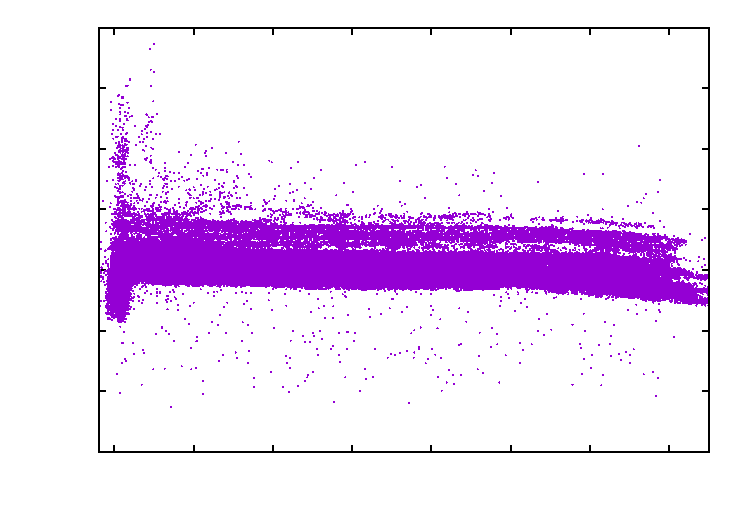
\includegraphics{temp_roh}}%
    \gplfronttext
  \end{picture}%
\endgroup
}}
	\hfill
	\subfigure[Temperaturverlauf aller Messungen des Northeimer Sees aufgetragen gegen die Tiefe mit einem abschnittsweise linearen Fit. Die ersten Messwerte bei 0\si{\meter} ergeben sich beim Eintauchen der Sonde und sind deswegen nicht beachtet.\label{fig:temp_nor}]
	{\resizebox{0.59\textwidth}{!}{% GNUPLOT: LaTeX picture with Postscript
\begingroup
  \makeatletter
  \providecommand\color[2][]{%
    \GenericError{(gnuplot) \space\space\space\@spaces}{%
      Package color not loaded in conjunction with
      terminal option `colourtext'%
    }{See the gnuplot documentation for explanation.%
    }{Either use 'blacktext' in gnuplot or load the package
      color.sty in LaTeX.}%
    \renewcommand\color[2][]{}%
  }%
  \providecommand\includegraphics[2][]{%
    \GenericError{(gnuplot) \space\space\space\@spaces}{%
      Package graphicx or graphics not loaded%
    }{See the gnuplot documentation for explanation.%
    }{The gnuplot epslatex terminal needs graphicx.sty or graphics.sty.}%
    \renewcommand\includegraphics[2][]{}%
  }%
  \providecommand\rotatebox[2]{#2}%
  \@ifundefined{ifGPcolor}{%
    \newif\ifGPcolor
    \GPcolortrue
  }{}%
  \@ifundefined{ifGPblacktext}{%
    \newif\ifGPblacktext
    \GPblacktexttrue
  }{}%
  % define a \g@addto@macro without @ in the name:
  \let\gplgaddtomacro\g@addto@macro
  % define empty templates for all commands taking text:
  \gdef\gplbacktext{}%
  \gdef\gplfronttext{}%
  \makeatother
  \ifGPblacktext
    % no textcolor at all
    \def\colorrgb#1{}%
    \def\colorgray#1{}%
  \else
    % gray or color?
    \ifGPcolor
      \def\colorrgb#1{\color[rgb]{#1}}%
      \def\colorgray#1{\color[gray]{#1}}%
      \expandafter\def\csname LTw\endcsname{\color{white}}%
      \expandafter\def\csname LTb\endcsname{\color{black}}%
      \expandafter\def\csname LTa\endcsname{\color{black}}%
      \expandafter\def\csname LT0\endcsname{\color[rgb]{1,0,0}}%
      \expandafter\def\csname LT1\endcsname{\color[rgb]{0,1,0}}%
      \expandafter\def\csname LT2\endcsname{\color[rgb]{0,0,1}}%
      \expandafter\def\csname LT3\endcsname{\color[rgb]{1,0,1}}%
      \expandafter\def\csname LT4\endcsname{\color[rgb]{0,1,1}}%
      \expandafter\def\csname LT5\endcsname{\color[rgb]{1,1,0}}%
      \expandafter\def\csname LT6\endcsname{\color[rgb]{0,0,0}}%
      \expandafter\def\csname LT7\endcsname{\color[rgb]{1,0.3,0}}%
      \expandafter\def\csname LT8\endcsname{\color[rgb]{0.5,0.5,0.5}}%
    \else
      % gray
      \def\colorrgb#1{\color{black}}%
      \def\colorgray#1{\color[gray]{#1}}%
      \expandafter\def\csname LTw\endcsname{\color{white}}%
      \expandafter\def\csname LTb\endcsname{\color{black}}%
      \expandafter\def\csname LTa\endcsname{\color{black}}%
      \expandafter\def\csname LT0\endcsname{\color{black}}%
      \expandafter\def\csname LT1\endcsname{\color{black}}%
      \expandafter\def\csname LT2\endcsname{\color{black}}%
      \expandafter\def\csname LT3\endcsname{\color{black}}%
      \expandafter\def\csname LT4\endcsname{\color{black}}%
      \expandafter\def\csname LT5\endcsname{\color{black}}%
      \expandafter\def\csname LT6\endcsname{\color{black}}%
      \expandafter\def\csname LT7\endcsname{\color{black}}%
      \expandafter\def\csname LT8\endcsname{\color{black}}%
    \fi
  \fi
  \setlength{\unitlength}{0.0500bp}%
  \begin{picture}(7200.00,5040.00)%
    \gplgaddtomacro\gplbacktext{%
      \csname LTb\endcsname%
      \put(814,1017){\makebox(0,0)[r]{\strut{} 15}}%
      \put(814,1643){\makebox(0,0)[r]{\strut{} 16}}%
      \put(814,2270){\makebox(0,0)[r]{\strut{} 17}}%
      \put(814,2896){\makebox(0,0)[r]{\strut{} 18}}%
      \put(814,3522){\makebox(0,0)[r]{\strut{} 19}}%
      \put(814,4149){\makebox(0,0)[r]{\strut{} 20}}%
      \put(814,4775){\makebox(0,0)[r]{\strut{} 21}}%
      \put(1098,484){\makebox(0,0){\strut{} 0}}%
      \put(1859,484){\makebox(0,0){\strut{} 1}}%
      \put(2619,484){\makebox(0,0){\strut{} 2}}%
      \put(3380,484){\makebox(0,0){\strut{} 3}}%
      \put(4141,484){\makebox(0,0){\strut{} 4}}%
      \put(4901,484){\makebox(0,0){\strut{} 5}}%
      \put(5662,484){\makebox(0,0){\strut{} 6}}%
      \put(6423,484){\makebox(0,0){\strut{} 7}}%
      \put(176,2739){\rotatebox{-270}{\makebox(0,0){\strut{}$T$ [$\si{\celsius}$]}}}%
      \put(3874,154){\makebox(0,0){\strut{}$z$ [m]}}%
    }%
    \gplgaddtomacro\gplfronttext{%
      \csname LTb\endcsname%
      \put(5816,4602){\makebox(0,0)[r]{\strut{}bereinigte Daten}}%
      \csname LTb\endcsname%
      \put(5816,4382){\makebox(0,0)[r]{\strut{}Approximation}}%
    }%
    \gplbacktext
    \put(0,0){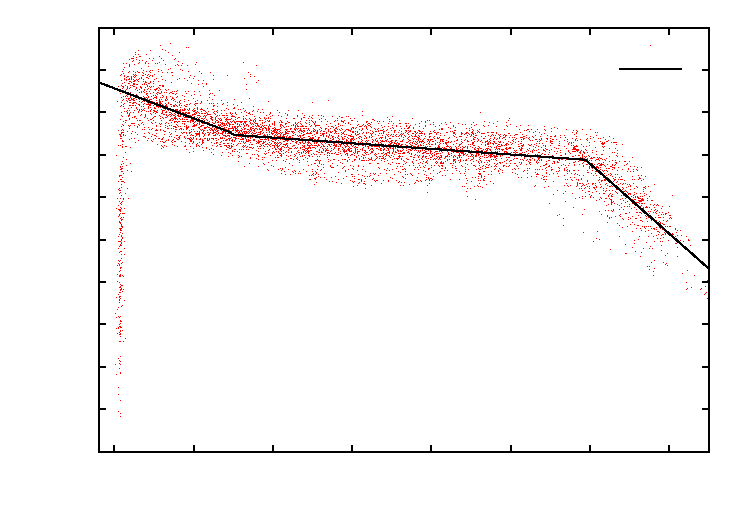
\includegraphics{temp}}%
    \gplfronttext
  \end{picture}%
\endgroup
}}
	\caption{Temperaturmessung Northeim.}
	\label{fig:temp_Nord}
\end{figure}

In Grafik \ref{fig:temp_nor_Roh} sind alle Temperaturmessungen der Messung in Northeim aufgetragen.
Man erkennt deutlich mehrere Linien.
Um dies zu beheben und die richtigen Daten zu verwenden, müssen sie gefiltert werden.
Dabei werden immer 40 Werte nach dem folgenden Algorithmus zu einem Temperaturwert zusammengefasst: 
Zuerst wird der Median bestimmt; nun werden nur noch Werte unterhalb dessen betrachtet, der Median ist also $T_\text{max}$. 
Außerdem schließt man Ausreißer nach unten aus, indem der untere Quartilwert$-3\si{\celsius}$ als $T_\text{min}$ verwendet wird.
Von den verbleibenden Werten wird der Mittelwert genommen.
Dieses Verfahren wird in Abb. \ref{fig:tempAlg} verdeutlicht.

\begin{figure}[!h]
	\centering
	\subfigure[Beispiel 1 \label{fig:tempAlg1l}]
   {\resizebox{0.49\linewidth}{!}{% GNUPLOT: LaTeX picture with Postscript
\begingroup
  \makeatletter
  \providecommand\color[2][]{%
    \GenericError{(gnuplot) \space\space\space\@spaces}{%
      Package color not loaded in conjunction with
      terminal option `colourtext'%
    }{See the gnuplot documentation for explanation.%
    }{Either use 'blacktext' in gnuplot or load the package
      color.sty in LaTeX.}%
    \renewcommand\color[2][]{}%
  }%
  \providecommand\includegraphics[2][]{%
    \GenericError{(gnuplot) \space\space\space\@spaces}{%
      Package graphicx or graphics not loaded%
    }{See the gnuplot documentation for explanation.%
    }{The gnuplot epslatex terminal needs graphicx.sty or graphics.sty.}%
    \renewcommand\includegraphics[2][]{}%
  }%
  \providecommand\rotatebox[2]{#2}%
  \@ifundefined{ifGPcolor}{%
    \newif\ifGPcolor
    \GPcolortrue
  }{}%
  \@ifundefined{ifGPblacktext}{%
    \newif\ifGPblacktext
    \GPblacktexttrue
  }{}%
  % define a \g@addto@macro without @ in the name:
  \let\gplgaddtomacro\g@addto@macro
  % define empty templates for all commands taking text:
  \gdef\gplbacktext{}%
  \gdef\gplfronttext{}%
  \makeatother
  \ifGPblacktext
    % no textcolor at all
    \def\colorrgb#1{}%
    \def\colorgray#1{}%
  \else
    % gray or color?
    \ifGPcolor
      \def\colorrgb#1{\color[rgb]{#1}}%
      \def\colorgray#1{\color[gray]{#1}}%
      \expandafter\def\csname LTw\endcsname{\color{white}}%
      \expandafter\def\csname LTb\endcsname{\color{black}}%
      \expandafter\def\csname LTa\endcsname{\color{black}}%
      \expandafter\def\csname LT0\endcsname{\color[rgb]{1,0,0}}%
      \expandafter\def\csname LT1\endcsname{\color[rgb]{0,1,0}}%
      \expandafter\def\csname LT2\endcsname{\color[rgb]{0,0,1}}%
      \expandafter\def\csname LT3\endcsname{\color[rgb]{1,0,1}}%
      \expandafter\def\csname LT4\endcsname{\color[rgb]{0,1,1}}%
      \expandafter\def\csname LT5\endcsname{\color[rgb]{1,1,0}}%
      \expandafter\def\csname LT6\endcsname{\color[rgb]{0,0,0}}%
      \expandafter\def\csname LT7\endcsname{\color[rgb]{1,0.3,0}}%
      \expandafter\def\csname LT8\endcsname{\color[rgb]{0.5,0.5,0.5}}%
    \else
      % gray
      \def\colorrgb#1{\color{black}}%
      \def\colorgray#1{\color[gray]{#1}}%
      \expandafter\def\csname LTw\endcsname{\color{white}}%
      \expandafter\def\csname LTb\endcsname{\color{black}}%
      \expandafter\def\csname LTa\endcsname{\color{black}}%
      \expandafter\def\csname LT0\endcsname{\color{black}}%
      \expandafter\def\csname LT1\endcsname{\color{black}}%
      \expandafter\def\csname LT2\endcsname{\color{black}}%
      \expandafter\def\csname LT3\endcsname{\color{black}}%
      \expandafter\def\csname LT4\endcsname{\color{black}}%
      \expandafter\def\csname LT5\endcsname{\color{black}}%
      \expandafter\def\csname LT6\endcsname{\color{black}}%
      \expandafter\def\csname LT7\endcsname{\color{black}}%
      \expandafter\def\csname LT8\endcsname{\color{black}}%
    \fi
  \fi
    \setlength{\unitlength}{0.0500bp}%
    \ifx\gptboxheight\undefined%
      \newlength{\gptboxheight}%
      \newlength{\gptboxwidth}%
      \newsavebox{\gptboxtext}%
    \fi%
    \setlength{\fboxrule}{0.5pt}%
    \setlength{\fboxsep}{1pt}%
\begin{picture}(7200.00,5040.00)%
    \gplgaddtomacro\gplbacktext{%
      \csname LTb\endcsname%
      \put(462,440){\makebox(0,0)[r]{\strut{}$14$}}%
      \put(462,1059){\makebox(0,0)[r]{\strut{}$16$}}%
      \put(462,1679){\makebox(0,0)[r]{\strut{}$18$}}%
      \put(462,2298){\makebox(0,0)[r]{\strut{}$20$}}%
      \put(462,2917){\makebox(0,0)[r]{\strut{}$22$}}%
      \put(462,3536){\makebox(0,0)[r]{\strut{}$24$}}%
      \put(462,4156){\makebox(0,0)[r]{\strut{}$26$}}%
      \put(462,4775){\makebox(0,0)[r]{\strut{}$28$}}%
      \put(594,220){\makebox(0,0){\strut{}$1200$}}%
      \put(1390,220){\makebox(0,0){\strut{}$1205$}}%
      \put(2186,220){\makebox(0,0){\strut{}$1210$}}%
      \put(2982,220){\makebox(0,0){\strut{}$1215$}}%
      \put(3778,220){\makebox(0,0){\strut{}$1220$}}%
      \put(4574,220){\makebox(0,0){\strut{}$1225$}}%
      \put(5370,220){\makebox(0,0){\strut{}$1230$}}%
      \put(6166,220){\makebox(0,0){\strut{}$1235$}}%
    }%
    \gplgaddtomacro\gplfronttext{%
      \csname LTb\endcsname%
      \put(2442,4602){\makebox(0,0)[r]{\strut{}Rohdaten}}%
      \csname LTb\endcsname%
      \put(2442,4382){\makebox(0,0)[r]{\strut{}$T_{min}$}}%
      \csname LTb\endcsname%
      \put(2442,4162){\makebox(0,0)[r]{\strut{}$T_{max}$ (Median)}}%
      \csname LTb\endcsname%
      \put(2442,3942){\makebox(0,0)[r]{\strut{}Approximation}}%
    }%
    \gplbacktext
    \put(0,0){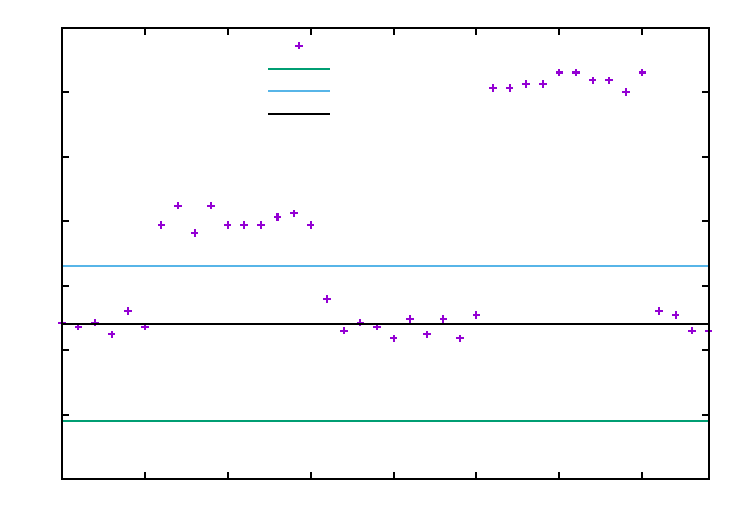
\includegraphics{tempAlg1}}%
    \gplfronttext
  \end{picture}%
\endgroup
}}
   \hfill
   \subfigure[Beispiel 2\label{fig:tempV1}]
   {\resizebox{.49\linewidth}{!}{% GNUPLOT: LaTeX picture with Postscript
\begingroup
  \makeatletter
  \providecommand\color[2][]{%
    \GenericError{(gnuplot) \space\space\space\@spaces}{%
      Package color not loaded in conjunction with
      terminal option `colourtext'%
    }{See the gnuplot documentation for explanation.%
    }{Either use 'blacktext' in gnuplot or load the package
      color.sty in LaTeX.}%
    \renewcommand\color[2][]{}%
  }%
  \providecommand\includegraphics[2][]{%
    \GenericError{(gnuplot) \space\space\space\@spaces}{%
      Package graphicx or graphics not loaded%
    }{See the gnuplot documentation for explanation.%
    }{The gnuplot epslatex terminal needs graphicx.sty or graphics.sty.}%
    \renewcommand\includegraphics[2][]{}%
  }%
  \providecommand\rotatebox[2]{#2}%
  \@ifundefined{ifGPcolor}{%
    \newif\ifGPcolor
    \GPcolortrue
  }{}%
  \@ifundefined{ifGPblacktext}{%
    \newif\ifGPblacktext
    \GPblacktexttrue
  }{}%
  % define a \g@addto@macro without @ in the name:
  \let\gplgaddtomacro\g@addto@macro
  % define empty templates for all commands taking text:
  \gdef\gplbacktext{}%
  \gdef\gplfronttext{}%
  \makeatother
  \ifGPblacktext
    % no textcolor at all
    \def\colorrgb#1{}%
    \def\colorgray#1{}%
  \else
    % gray or color?
    \ifGPcolor
      \def\colorrgb#1{\color[rgb]{#1}}%
      \def\colorgray#1{\color[gray]{#1}}%
      \expandafter\def\csname LTw\endcsname{\color{white}}%
      \expandafter\def\csname LTb\endcsname{\color{black}}%
      \expandafter\def\csname LTa\endcsname{\color{black}}%
      \expandafter\def\csname LT0\endcsname{\color[rgb]{1,0,0}}%
      \expandafter\def\csname LT1\endcsname{\color[rgb]{0,1,0}}%
      \expandafter\def\csname LT2\endcsname{\color[rgb]{0,0,1}}%
      \expandafter\def\csname LT3\endcsname{\color[rgb]{1,0,1}}%
      \expandafter\def\csname LT4\endcsname{\color[rgb]{0,1,1}}%
      \expandafter\def\csname LT5\endcsname{\color[rgb]{1,1,0}}%
      \expandafter\def\csname LT6\endcsname{\color[rgb]{0,0,0}}%
      \expandafter\def\csname LT7\endcsname{\color[rgb]{1,0.3,0}}%
      \expandafter\def\csname LT8\endcsname{\color[rgb]{0.5,0.5,0.5}}%
    \else
      % gray
      \def\colorrgb#1{\color{black}}%
      \def\colorgray#1{\color[gray]{#1}}%
      \expandafter\def\csname LTw\endcsname{\color{white}}%
      \expandafter\def\csname LTb\endcsname{\color{black}}%
      \expandafter\def\csname LTa\endcsname{\color{black}}%
      \expandafter\def\csname LT0\endcsname{\color{black}}%
      \expandafter\def\csname LT1\endcsname{\color{black}}%
      \expandafter\def\csname LT2\endcsname{\color{black}}%
      \expandafter\def\csname LT3\endcsname{\color{black}}%
      \expandafter\def\csname LT4\endcsname{\color{black}}%
      \expandafter\def\csname LT5\endcsname{\color{black}}%
      \expandafter\def\csname LT6\endcsname{\color{black}}%
      \expandafter\def\csname LT7\endcsname{\color{black}}%
      \expandafter\def\csname LT8\endcsname{\color{black}}%
    \fi
  \fi
    \setlength{\unitlength}{0.0500bp}%
    \ifx\gptboxheight\undefined%
      \newlength{\gptboxheight}%
      \newlength{\gptboxwidth}%
      \newsavebox{\gptboxtext}%
    \fi%
    \setlength{\fboxrule}{0.5pt}%
    \setlength{\fboxsep}{1pt}%
\begin{picture}(7200.00,5040.00)%
    \gplgaddtomacro\gplbacktext{%
      \csname LTb\endcsname%
      \put(726,440){\makebox(0,0)[r]{\strut{}$15$}}%
      \put(726,834){\makebox(0,0)[r]{\strut{}$15.5$}}%
      \put(726,1228){\makebox(0,0)[r]{\strut{}$16$}}%
      \put(726,1622){\makebox(0,0)[r]{\strut{}$16.5$}}%
      \put(726,2016){\makebox(0,0)[r]{\strut{}$17$}}%
      \put(726,2410){\makebox(0,0)[r]{\strut{}$17.5$}}%
      \put(726,2805){\makebox(0,0)[r]{\strut{}$18$}}%
      \put(726,3199){\makebox(0,0)[r]{\strut{}$18.5$}}%
      \put(726,3593){\makebox(0,0)[r]{\strut{}$19$}}%
      \put(726,3987){\makebox(0,0)[r]{\strut{}$19.5$}}%
      \put(726,4381){\makebox(0,0)[r]{\strut{}$20$}}%
      \put(726,4775){\makebox(0,0)[r]{\strut{}$20.5$}}%
      \put(858,220){\makebox(0,0){\strut{}$3600$}}%
      \put(1620,220){\makebox(0,0){\strut{}$3605$}}%
      \put(2382,220){\makebox(0,0){\strut{}$3610$}}%
      \put(3145,220){\makebox(0,0){\strut{}$3615$}}%
      \put(3907,220){\makebox(0,0){\strut{}$3620$}}%
      \put(4669,220){\makebox(0,0){\strut{}$3625$}}%
      \put(5431,220){\makebox(0,0){\strut{}$3630$}}%
      \put(6193,220){\makebox(0,0){\strut{}$3635$}}%
    }%
    \gplgaddtomacro\gplfronttext{%
      \csname LTb\endcsname%
      \put(5816,1273){\makebox(0,0)[r]{\strut{}Rohdaten}}%
      \csname LTb\endcsname%
      \put(5816,1053){\makebox(0,0)[r]{\strut{}$T_{min}$}}%
      \csname LTb\endcsname%
      \put(5816,833){\makebox(0,0)[r]{\strut{}$T_{max}$ (Median)}}%
      \csname LTb\endcsname%
      \put(5816,613){\makebox(0,0)[r]{\strut{}Approximation}}%
    }%
    \gplbacktext
    \put(0,0){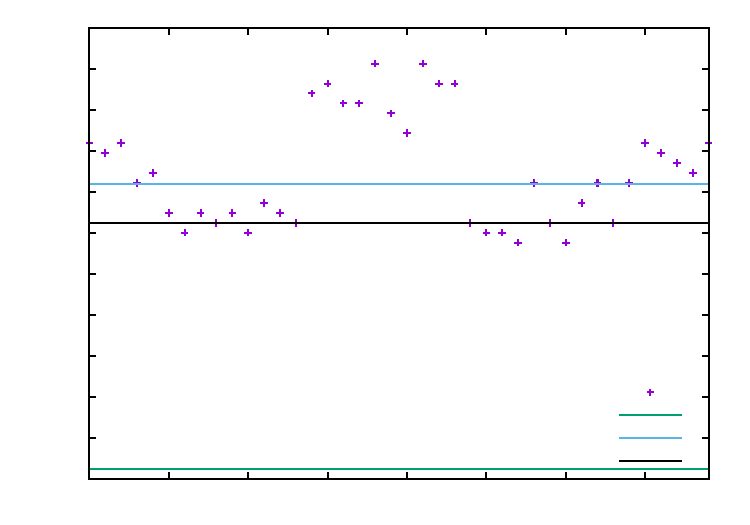
\includegraphics{tempAlg2}}%
    \gplfronttext
  \end{picture}%
\endgroup
}}
	\caption{Algorithmus zum Filtern der Temperaturdaten. Es sind in beiden Plots die Sprünge, sowie die Korrekturen in der Temperatur gut zu erkennen.}
	\label{fig:tempAlg}
\end{figure}

Das Resultat des Filtervorgangs ist in Abb. \ref{fig:temp_nor} zu sehen.
Wieder wurden alle Daten in einen Plot eingezeichnet, denn der See schien  im Rahmen der Messfehler homogen.
Man erkennt drei verschiedene Bereiche: $0.2-1.5\,$m, $1.5-5.9\,$m und $5.9-7.5\,$m.
Die gefittete Kurve besteht aus drei linearen Fits, welche in den einzelnen Bereichen durchgeführt werden.
Es ergeben sich die Werte aus Tabelle \ref{tab:tempTabNor}.

\begin{table}[!htb]
\centering
\begin{tabular}{|c||c|c|}
\hline
Tiefe [m] & Temperaturabnahme [$\frac{^\circ C}{\text m}$] & Temperaturintervall [$^\circ$C]\\\hline\hline
0.2 - 1.5 & $-0.71\pm  0.03$	& 19.4 - 18.5 \\
1.5 - 5.9 & $-0.132\pm 0.005$	& 18.5 - 17.9 \\
5.9 - 7.5 & $-1.65\pm 0.04$	& 18.0 - 15.3 \\\hline
\end{tabular}
\caption{Temperaturkoeffizienten aus dem Fit von Abb. \ref{fig:temp_nor}.}
\label{tab:tempTabNor}
\end{table}


Da wir in der App die vorherigen Messpositionen auf einer Karte sehen konnten, haben wir drei Positionen noch ein zweites Mal besucht, um vergleichen zu können, wie sich der See mit der Zeit erwärmt.
Diese sind in der Karte \ref{fig:GPSNortZweimal} eingezeichnet.
Vergleicht man jeweils die beiden Temperaturkurven in Abb. \ref{fig:tempV1} bis \ref{fig:tempV3}, erkennt man keine großen Temperaturdifferenzen.
Die Messfehler scheinen zu überwiegen.
Eventuell kann man in der Abb.\ref{fig:tempV3} erkennen, dass sich die Seeoberfläche leicht erwärmt hat
Für eine genauere Analyse hätte man jedoch über einen längeren Zeitraum messen müssen.
In Abb. \ref{fig:tempV2} ist die später aufgenommene Kurve etwa $0.5\si\celsius$ unter der anderen.
Dies kann verschiedene Gründe haben: Zum einen kann dies ein Fehler des obigen Filteralgorithmus sein, zum anderen könnte es auf Messfehler zurückzuführen sein, denn eine so starke Abkühlung scheint nicht plausibel.
Wir erwarten nämlich eine Erwärmung, da an diesem Tag die Sonne gut gescheint hat.
Auffällig ist auch, dass die zweite Messreihe etwa 1.5 Meter kürzer ist, der See in dieser Region also steil abzufallen scheint.
Diese Veränderung zu messen, wäre sicherlich auch interessant.

\begin{figure}[!htb]
	\centering
	\subfigure[Karte. \label{fig:GPSNortZweimal}]
   {\resizebox{0.49\linewidth}{!}{% GNUPLOT: LaTeX picture with Postscript
\begingroup
  \makeatletter
  \providecommand\color[2][]{%
    \GenericError{(gnuplot) \space\space\space\@spaces}{%
      Package color not loaded in conjunction with
      terminal option `colourtext'%
    }{See the gnuplot documentation for explanation.%
    }{Either use 'blacktext' in gnuplot or load the package
      color.sty in LaTeX.}%
    \renewcommand\color[2][]{}%
  }%
  \providecommand\includegraphics[2][]{%
    \GenericError{(gnuplot) \space\space\space\@spaces}{%
      Package graphicx or graphics not loaded%
    }{See the gnuplot documentation for explanation.%
    }{The gnuplot epslatex terminal needs graphicx.sty or graphics.sty.}%
    \renewcommand\includegraphics[2][]{}%
  }%
  \providecommand\rotatebox[2]{#2}%
  \@ifundefined{ifGPcolor}{%
    \newif\ifGPcolor
    \GPcolortrue
  }{}%
  \@ifundefined{ifGPblacktext}{%
    \newif\ifGPblacktext
    \GPblacktexttrue
  }{}%
  % define a \g@addto@macro without @ in the name:
  \let\gplgaddtomacro\g@addto@macro
  % define empty templates for all commands taking text:
  \gdef\gplbacktext{}%
  \gdef\gplfronttext{}%
  \makeatother
  \ifGPblacktext
    % no textcolor at all
    \def\colorrgb#1{}%
    \def\colorgray#1{}%
  \else
    % gray or color?
    \ifGPcolor
      \def\colorrgb#1{\color[rgb]{#1}}%
      \def\colorgray#1{\color[gray]{#1}}%
      \expandafter\def\csname LTw\endcsname{\color{white}}%
      \expandafter\def\csname LTb\endcsname{\color{black}}%
      \expandafter\def\csname LTa\endcsname{\color{black}}%
      \expandafter\def\csname LT0\endcsname{\color[rgb]{1,0,0}}%
      \expandafter\def\csname LT1\endcsname{\color[rgb]{0,1,0}}%
      \expandafter\def\csname LT2\endcsname{\color[rgb]{0,0,1}}%
      \expandafter\def\csname LT3\endcsname{\color[rgb]{1,0,1}}%
      \expandafter\def\csname LT4\endcsname{\color[rgb]{0,1,1}}%
      \expandafter\def\csname LT5\endcsname{\color[rgb]{1,1,0}}%
      \expandafter\def\csname LT6\endcsname{\color[rgb]{0,0,0}}%
      \expandafter\def\csname LT7\endcsname{\color[rgb]{1,0.3,0}}%
      \expandafter\def\csname LT8\endcsname{\color[rgb]{0.5,0.5,0.5}}%
    \else
      % gray
      \def\colorrgb#1{\color{black}}%
      \def\colorgray#1{\color[gray]{#1}}%
      \expandafter\def\csname LTw\endcsname{\color{white}}%
      \expandafter\def\csname LTb\endcsname{\color{black}}%
      \expandafter\def\csname LTa\endcsname{\color{black}}%
      \expandafter\def\csname LT0\endcsname{\color{black}}%
      \expandafter\def\csname LT1\endcsname{\color{black}}%
      \expandafter\def\csname LT2\endcsname{\color{black}}%
      \expandafter\def\csname LT3\endcsname{\color{black}}%
      \expandafter\def\csname LT4\endcsname{\color{black}}%
      \expandafter\def\csname LT5\endcsname{\color{black}}%
      \expandafter\def\csname LT6\endcsname{\color{black}}%
      \expandafter\def\csname LT7\endcsname{\color{black}}%
      \expandafter\def\csname LT8\endcsname{\color{black}}%
    \fi
  \fi
  \setlength{\unitlength}{0.0500bp}%
  \begin{picture}(7200.00,5040.00)%
    \gplgaddtomacro\gplbacktext{%
      \csname LTb\endcsname%
      \put(1307,704){\makebox(0,0)[r]{\strut{}-800}}%
      \put(1307,1444){\makebox(0,0)[r]{\strut{}-700}}%
      \put(1307,2184){\makebox(0,0)[r]{\strut{}-600}}%
      \put(1307,2925){\makebox(0,0)[r]{\strut{}-500}}%
      \put(1307,3665){\makebox(0,0)[r]{\strut{}-400}}%
      \put(1307,4405){\makebox(0,0)[r]{\strut{}-300}}%
      \put(1439,484){\makebox(0,0){\strut{} 0}}%
      \put(1809,484){\makebox(0,0){\strut{} 50}}%
      \put(2179,484){\makebox(0,0){\strut{} 100}}%
      \put(2549,484){\makebox(0,0){\strut{} 150}}%
      \put(2919,484){\makebox(0,0){\strut{} 200}}%
      \put(3289,484){\makebox(0,0){\strut{} 250}}%
      \put(3659,484){\makebox(0,0){\strut{} 300}}%
      \put(4029,484){\makebox(0,0){\strut{} 350}}%
      \put(4399,484){\makebox(0,0){\strut{} 400}}%
      \put(537,2739){\rotatebox{-270}{\makebox(0,0){\strut{}y [m]}}}%
      \put(2919,154){\makebox(0,0){\strut{}x [m]}}%
      \put(2179,4627){\makebox(0,0)[l]{\strut{}Insel}}%
      \put(3955,3110){\makebox(0,0)[l]{\strut{}N}}%
    }%
    \gplgaddtomacro\gplfronttext{%
      \csname LTb\endcsname%
      \put(6212,3289){\makebox(0,0)[r]{\strut{}12:59 Uhr}}%
      \csname LTb\endcsname%
      \put(6212,3069){\makebox(0,0)[r]{\strut{}14:46 Uhr}}%
      \csname LTb\endcsname%
      \put(6212,2849){\makebox(0,0)[r]{\strut{}13:16 Uhr}}%
      \csname LTb\endcsname%
      \put(6212,2629){\makebox(0,0)[r]{\strut{}14:42 Uhr}}%
      \csname LTb\endcsname%
      \put(6212,2409){\makebox(0,0)[r]{\strut{}12:39 Uhr}}%
      \csname LTb\endcsname%
      \put(6212,2189){\makebox(0,0)[r]{\strut{}14:53 Uhr}}%
    }%
    \gplbacktext
    \put(0,0){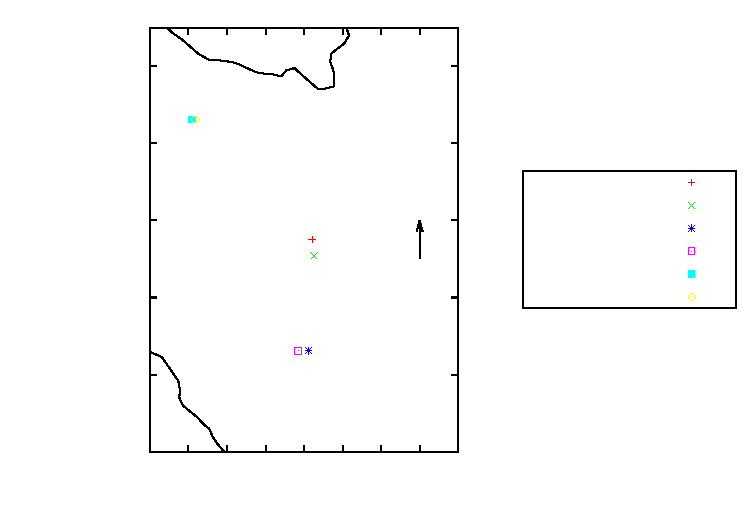
\includegraphics{karte2}}%
    \gplfronttext
  \end{picture}%
\endgroup
}}
   \hfill
   \subfigure[Verlauf 1.\label{fig:tempV1}]
   {\resizebox{.49\linewidth}{!}{% GNUPLOT: LaTeX picture with Postscript
\begingroup
  \makeatletter
  \providecommand\color[2][]{%
    \GenericError{(gnuplot) \space\space\space\@spaces}{%
      Package color not loaded in conjunction with
      terminal option `colourtext'%
    }{See the gnuplot documentation for explanation.%
    }{Either use 'blacktext' in gnuplot or load the package
      color.sty in LaTeX.}%
    \renewcommand\color[2][]{}%
  }%
  \providecommand\includegraphics[2][]{%
    \GenericError{(gnuplot) \space\space\space\@spaces}{%
      Package graphicx or graphics not loaded%
    }{See the gnuplot documentation for explanation.%
    }{The gnuplot epslatex terminal needs graphicx.sty or graphics.sty.}%
    \renewcommand\includegraphics[2][]{}%
  }%
  \providecommand\rotatebox[2]{#2}%
  \@ifundefined{ifGPcolor}{%
    \newif\ifGPcolor
    \GPcolortrue
  }{}%
  \@ifundefined{ifGPblacktext}{%
    \newif\ifGPblacktext
    \GPblacktexttrue
  }{}%
  % define a \g@addto@macro without @ in the name:
  \let\gplgaddtomacro\g@addto@macro
  % define empty templates for all commands taking text:
  \gdef\gplbacktext{}%
  \gdef\gplfronttext{}%
  \makeatother
  \ifGPblacktext
    % no textcolor at all
    \def\colorrgb#1{}%
    \def\colorgray#1{}%
  \else
    % gray or color?
    \ifGPcolor
      \def\colorrgb#1{\color[rgb]{#1}}%
      \def\colorgray#1{\color[gray]{#1}}%
      \expandafter\def\csname LTw\endcsname{\color{white}}%
      \expandafter\def\csname LTb\endcsname{\color{black}}%
      \expandafter\def\csname LTa\endcsname{\color{black}}%
      \expandafter\def\csname LT0\endcsname{\color[rgb]{1,0,0}}%
      \expandafter\def\csname LT1\endcsname{\color[rgb]{0,1,0}}%
      \expandafter\def\csname LT2\endcsname{\color[rgb]{0,0,1}}%
      \expandafter\def\csname LT3\endcsname{\color[rgb]{1,0,1}}%
      \expandafter\def\csname LT4\endcsname{\color[rgb]{0,1,1}}%
      \expandafter\def\csname LT5\endcsname{\color[rgb]{1,1,0}}%
      \expandafter\def\csname LT6\endcsname{\color[rgb]{0,0,0}}%
      \expandafter\def\csname LT7\endcsname{\color[rgb]{1,0.3,0}}%
      \expandafter\def\csname LT8\endcsname{\color[rgb]{0.5,0.5,0.5}}%
    \else
      % gray
      \def\colorrgb#1{\color{black}}%
      \def\colorgray#1{\color[gray]{#1}}%
      \expandafter\def\csname LTw\endcsname{\color{white}}%
      \expandafter\def\csname LTb\endcsname{\color{black}}%
      \expandafter\def\csname LTa\endcsname{\color{black}}%
      \expandafter\def\csname LT0\endcsname{\color{black}}%
      \expandafter\def\csname LT1\endcsname{\color{black}}%
      \expandafter\def\csname LT2\endcsname{\color{black}}%
      \expandafter\def\csname LT3\endcsname{\color{black}}%
      \expandafter\def\csname LT4\endcsname{\color{black}}%
      \expandafter\def\csname LT5\endcsname{\color{black}}%
      \expandafter\def\csname LT6\endcsname{\color{black}}%
      \expandafter\def\csname LT7\endcsname{\color{black}}%
      \expandafter\def\csname LT8\endcsname{\color{black}}%
    \fi
  \fi
  \setlength{\unitlength}{0.0500bp}%
  \begin{picture}(7200.00,5040.00)%
    \gplgaddtomacro\gplbacktext{%
      \csname LTb\endcsname%
      \put(1078,704){\makebox(0,0)[r]{\strut{} 15.5}}%
      \put(1078,1111){\makebox(0,0)[r]{\strut{} 16}}%
      \put(1078,1518){\makebox(0,0)[r]{\strut{} 16.5}}%
      \put(1078,1925){\makebox(0,0)[r]{\strut{} 17}}%
      \put(1078,2332){\makebox(0,0)[r]{\strut{} 17.5}}%
      \put(1078,2740){\makebox(0,0)[r]{\strut{} 18}}%
      \put(1078,3147){\makebox(0,0)[r]{\strut{} 18.5}}%
      \put(1078,3554){\makebox(0,0)[r]{\strut{} 19}}%
      \put(1078,3961){\makebox(0,0)[r]{\strut{} 19.5}}%
      \put(1078,4368){\makebox(0,0)[r]{\strut{} 20}}%
      \put(1078,4775){\makebox(0,0)[r]{\strut{} 20.5}}%
      \put(1355,484){\makebox(0,0){\strut{} 0}}%
      \put(2082,484){\makebox(0,0){\strut{} 1}}%
      \put(2808,484){\makebox(0,0){\strut{} 2}}%
      \put(3534,484){\makebox(0,0){\strut{} 3}}%
      \put(4261,484){\makebox(0,0){\strut{} 4}}%
      \put(4987,484){\makebox(0,0){\strut{} 5}}%
      \put(5713,484){\makebox(0,0){\strut{} 6}}%
      \put(6440,484){\makebox(0,0){\strut{} 7}}%
      \put(176,2739){\rotatebox{-270}{\makebox(0,0){\strut{}$T$ [$\si{\celsius}$]}}}%
      \put(4006,154){\makebox(0,0){\strut{}$z$ [m]}}%
    }%
    \gplgaddtomacro\gplfronttext{%
      \csname LTb\endcsname%
      \put(5816,4602){\makebox(0,0)[r]{\strut{}12:59 Uhr}}%
      \csname LTb\endcsname%
      \put(5816,4382){\makebox(0,0)[r]{\strut{}14:46 Uhr}}%
    }%
    \gplbacktext
    \put(0,0){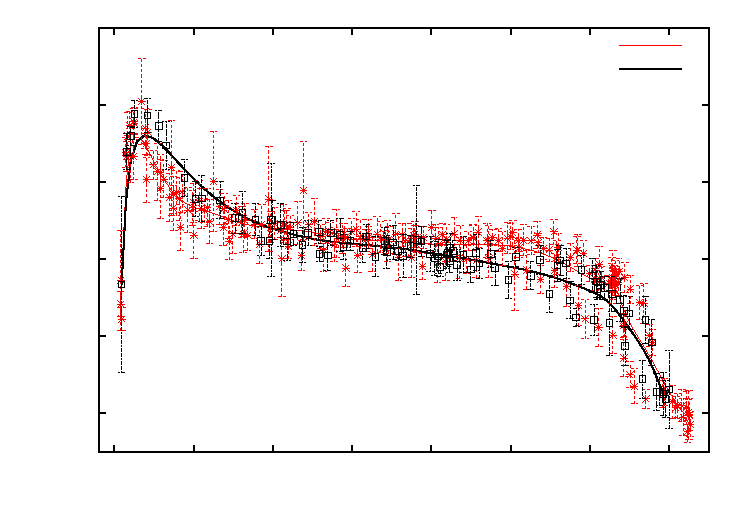
\includegraphics{tempV1}}%
    \gplfronttext
  \end{picture}%
\endgroup
}}
   \hfill
   \subfigure[Verlauf 2.\label{fig:tempV2}]
   {\resizebox{.49\linewidth}{!}{% GNUPLOT: LaTeX picture with Postscript
\begingroup
  \makeatletter
  \providecommand\color[2][]{%
    \GenericError{(gnuplot) \space\space\space\@spaces}{%
      Package color not loaded in conjunction with
      terminal option `colourtext'%
    }{See the gnuplot documentation for explanation.%
    }{Either use 'blacktext' in gnuplot or load the package
      color.sty in LaTeX.}%
    \renewcommand\color[2][]{}%
  }%
  \providecommand\includegraphics[2][]{%
    \GenericError{(gnuplot) \space\space\space\@spaces}{%
      Package graphicx or graphics not loaded%
    }{See the gnuplot documentation for explanation.%
    }{The gnuplot epslatex terminal needs graphicx.sty or graphics.sty.}%
    \renewcommand\includegraphics[2][]{}%
  }%
  \providecommand\rotatebox[2]{#2}%
  \@ifundefined{ifGPcolor}{%
    \newif\ifGPcolor
    \GPcolortrue
  }{}%
  \@ifundefined{ifGPblacktext}{%
    \newif\ifGPblacktext
    \GPblacktexttrue
  }{}%
  % define a \g@addto@macro without @ in the name:
  \let\gplgaddtomacro\g@addto@macro
  % define empty templates for all commands taking text:
  \gdef\gplbacktext{}%
  \gdef\gplfronttext{}%
  \makeatother
  \ifGPblacktext
    % no textcolor at all
    \def\colorrgb#1{}%
    \def\colorgray#1{}%
  \else
    % gray or color?
    \ifGPcolor
      \def\colorrgb#1{\color[rgb]{#1}}%
      \def\colorgray#1{\color[gray]{#1}}%
      \expandafter\def\csname LTw\endcsname{\color{white}}%
      \expandafter\def\csname LTb\endcsname{\color{black}}%
      \expandafter\def\csname LTa\endcsname{\color{black}}%
      \expandafter\def\csname LT0\endcsname{\color[rgb]{1,0,0}}%
      \expandafter\def\csname LT1\endcsname{\color[rgb]{0,1,0}}%
      \expandafter\def\csname LT2\endcsname{\color[rgb]{0,0,1}}%
      \expandafter\def\csname LT3\endcsname{\color[rgb]{1,0,1}}%
      \expandafter\def\csname LT4\endcsname{\color[rgb]{0,1,1}}%
      \expandafter\def\csname LT5\endcsname{\color[rgb]{1,1,0}}%
      \expandafter\def\csname LT6\endcsname{\color[rgb]{0,0,0}}%
      \expandafter\def\csname LT7\endcsname{\color[rgb]{1,0.3,0}}%
      \expandafter\def\csname LT8\endcsname{\color[rgb]{0.5,0.5,0.5}}%
    \else
      % gray
      \def\colorrgb#1{\color{black}}%
      \def\colorgray#1{\color[gray]{#1}}%
      \expandafter\def\csname LTw\endcsname{\color{white}}%
      \expandafter\def\csname LTb\endcsname{\color{black}}%
      \expandafter\def\csname LTa\endcsname{\color{black}}%
      \expandafter\def\csname LT0\endcsname{\color{black}}%
      \expandafter\def\csname LT1\endcsname{\color{black}}%
      \expandafter\def\csname LT2\endcsname{\color{black}}%
      \expandafter\def\csname LT3\endcsname{\color{black}}%
      \expandafter\def\csname LT4\endcsname{\color{black}}%
      \expandafter\def\csname LT5\endcsname{\color{black}}%
      \expandafter\def\csname LT6\endcsname{\color{black}}%
      \expandafter\def\csname LT7\endcsname{\color{black}}%
      \expandafter\def\csname LT8\endcsname{\color{black}}%
    \fi
  \fi
  \setlength{\unitlength}{0.0500bp}%
  \begin{picture}(7200.00,5040.00)%
    \gplgaddtomacro\gplbacktext{%
      \csname LTb\endcsname%
      \put(1078,704){\makebox(0,0)[r]{\strut{} 15.5}}%
      \put(1078,1156){\makebox(0,0)[r]{\strut{} 16}}%
      \put(1078,1609){\makebox(0,0)[r]{\strut{} 16.5}}%
      \put(1078,2061){\makebox(0,0)[r]{\strut{} 17}}%
      \put(1078,2513){\makebox(0,0)[r]{\strut{} 17.5}}%
      \put(1078,2966){\makebox(0,0)[r]{\strut{} 18}}%
      \put(1078,3418){\makebox(0,0)[r]{\strut{} 18.5}}%
      \put(1078,3870){\makebox(0,0)[r]{\strut{} 19}}%
      \put(1078,4323){\makebox(0,0)[r]{\strut{} 19.5}}%
      \put(1078,4775){\makebox(0,0)[r]{\strut{} 20}}%
      \put(1355,484){\makebox(0,0){\strut{} 0}}%
      \put(2082,484){\makebox(0,0){\strut{} 1}}%
      \put(2808,484){\makebox(0,0){\strut{} 2}}%
      \put(3534,484){\makebox(0,0){\strut{} 3}}%
      \put(4261,484){\makebox(0,0){\strut{} 4}}%
      \put(4987,484){\makebox(0,0){\strut{} 5}}%
      \put(5713,484){\makebox(0,0){\strut{} 6}}%
      \put(6440,484){\makebox(0,0){\strut{} 7}}%
      \put(176,2739){\rotatebox{-270}{\makebox(0,0){\strut{}$T$ [$\si{\celsius}$]}}}%
      \put(4006,154){\makebox(0,0){\strut{}$z$ [m]}}%
    }%
    \gplgaddtomacro\gplfronttext{%
      \csname LTb\endcsname%
      \put(5816,4602){\makebox(0,0)[r]{\strut{}13:16 Uhr}}%
      \csname LTb\endcsname%
      \put(5816,4382){\makebox(0,0)[r]{\strut{}14:42 Uhr}}%
    }%
    \gplbacktext
    \put(0,0){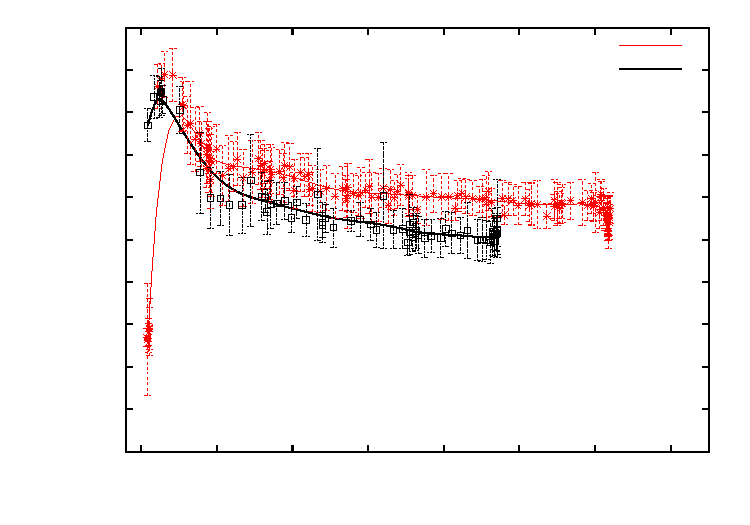
\includegraphics{tempV2}}%
    \gplfronttext
  \end{picture}%
\endgroup
}}
   \hfill
   \subfigure[Verlauf 3.\label{fig:tempV3}]
   {\resizebox{.49\linewidth}{!}{% GNUPLOT: LaTeX picture with Postscript
\begingroup
  \makeatletter
  \providecommand\color[2][]{%
    \GenericError{(gnuplot) \space\space\space\@spaces}{%
      Package color not loaded in conjunction with
      terminal option `colourtext'%
    }{See the gnuplot documentation for explanation.%
    }{Either use 'blacktext' in gnuplot or load the package
      color.sty in LaTeX.}%
    \renewcommand\color[2][]{}%
  }%
  \providecommand\includegraphics[2][]{%
    \GenericError{(gnuplot) \space\space\space\@spaces}{%
      Package graphicx or graphics not loaded%
    }{See the gnuplot documentation for explanation.%
    }{The gnuplot epslatex terminal needs graphicx.sty or graphics.sty.}%
    \renewcommand\includegraphics[2][]{}%
  }%
  \providecommand\rotatebox[2]{#2}%
  \@ifundefined{ifGPcolor}{%
    \newif\ifGPcolor
    \GPcolortrue
  }{}%
  \@ifundefined{ifGPblacktext}{%
    \newif\ifGPblacktext
    \GPblacktexttrue
  }{}%
  % define a \g@addto@macro without @ in the name:
  \let\gplgaddtomacro\g@addto@macro
  % define empty templates for all commands taking text:
  \gdef\gplbacktext{}%
  \gdef\gplfronttext{}%
  \makeatother
  \ifGPblacktext
    % no textcolor at all
    \def\colorrgb#1{}%
    \def\colorgray#1{}%
  \else
    % gray or color?
    \ifGPcolor
      \def\colorrgb#1{\color[rgb]{#1}}%
      \def\colorgray#1{\color[gray]{#1}}%
      \expandafter\def\csname LTw\endcsname{\color{white}}%
      \expandafter\def\csname LTb\endcsname{\color{black}}%
      \expandafter\def\csname LTa\endcsname{\color{black}}%
      \expandafter\def\csname LT0\endcsname{\color[rgb]{1,0,0}}%
      \expandafter\def\csname LT1\endcsname{\color[rgb]{0,1,0}}%
      \expandafter\def\csname LT2\endcsname{\color[rgb]{0,0,1}}%
      \expandafter\def\csname LT3\endcsname{\color[rgb]{1,0,1}}%
      \expandafter\def\csname LT4\endcsname{\color[rgb]{0,1,1}}%
      \expandafter\def\csname LT5\endcsname{\color[rgb]{1,1,0}}%
      \expandafter\def\csname LT6\endcsname{\color[rgb]{0,0,0}}%
      \expandafter\def\csname LT7\endcsname{\color[rgb]{1,0.3,0}}%
      \expandafter\def\csname LT8\endcsname{\color[rgb]{0.5,0.5,0.5}}%
    \else
      % gray
      \def\colorrgb#1{\color{black}}%
      \def\colorgray#1{\color[gray]{#1}}%
      \expandafter\def\csname LTw\endcsname{\color{white}}%
      \expandafter\def\csname LTb\endcsname{\color{black}}%
      \expandafter\def\csname LTa\endcsname{\color{black}}%
      \expandafter\def\csname LT0\endcsname{\color{black}}%
      \expandafter\def\csname LT1\endcsname{\color{black}}%
      \expandafter\def\csname LT2\endcsname{\color{black}}%
      \expandafter\def\csname LT3\endcsname{\color{black}}%
      \expandafter\def\csname LT4\endcsname{\color{black}}%
      \expandafter\def\csname LT5\endcsname{\color{black}}%
      \expandafter\def\csname LT6\endcsname{\color{black}}%
      \expandafter\def\csname LT7\endcsname{\color{black}}%
      \expandafter\def\csname LT8\endcsname{\color{black}}%
    \fi
  \fi
  \setlength{\unitlength}{0.0500bp}%
  \begin{picture}(7200.00,5040.00)%
    \gplgaddtomacro\gplbacktext{%
      \csname LTb\endcsname%
      \put(1078,704){\makebox(0,0)[r]{\strut{} 15.5}}%
      \put(1078,1111){\makebox(0,0)[r]{\strut{} 16}}%
      \put(1078,1518){\makebox(0,0)[r]{\strut{} 16.5}}%
      \put(1078,1925){\makebox(0,0)[r]{\strut{} 17}}%
      \put(1078,2332){\makebox(0,0)[r]{\strut{} 17.5}}%
      \put(1078,2740){\makebox(0,0)[r]{\strut{} 18}}%
      \put(1078,3147){\makebox(0,0)[r]{\strut{} 18.5}}%
      \put(1078,3554){\makebox(0,0)[r]{\strut{} 19}}%
      \put(1078,3961){\makebox(0,0)[r]{\strut{} 19.5}}%
      \put(1078,4368){\makebox(0,0)[r]{\strut{} 20}}%
      \put(1078,4775){\makebox(0,0)[r]{\strut{} 20.5}}%
      \put(1355,484){\makebox(0,0){\strut{} 0}}%
      \put(2082,484){\makebox(0,0){\strut{} 1}}%
      \put(2808,484){\makebox(0,0){\strut{} 2}}%
      \put(3534,484){\makebox(0,0){\strut{} 3}}%
      \put(4261,484){\makebox(0,0){\strut{} 4}}%
      \put(4987,484){\makebox(0,0){\strut{} 5}}%
      \put(5713,484){\makebox(0,0){\strut{} 6}}%
      \put(6440,484){\makebox(0,0){\strut{} 7}}%
      \put(176,2739){\rotatebox{-270}{\makebox(0,0){\strut{}$T$ [$\si{\celsius}$]}}}%
      \put(4006,154){\makebox(0,0){\strut{}$z$ [m]}}%
    }%
    \gplgaddtomacro\gplfronttext{%
      \csname LTb\endcsname%
      \put(5816,4602){\makebox(0,0)[r]{\strut{}12:39 Uhr}}%
      \csname LTb\endcsname%
      \put(5816,4382){\makebox(0,0)[r]{\strut{}14:53 Uhr}}%
    }%
    \gplbacktext
    \put(0,0){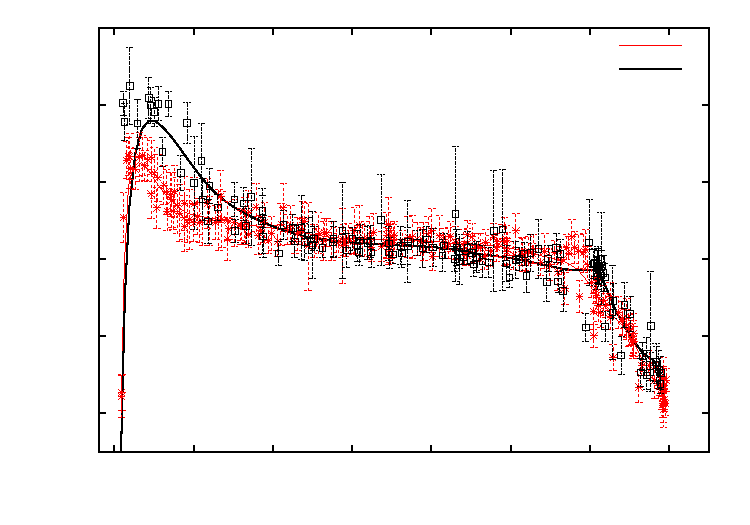
\includegraphics{tempV3}}%
    \gplfronttext
  \end{picture}%
\endgroup
}}
	\caption{Messpunkte in Northeim (in a), die wir zweimal besucht haben, und deren Temperaturkurven.}
	\label{fig:tempNort2}
\end{figure}


\subsection{Licht}

Bei den Daten der Photodiode zeigte sich in den Messdaten zu einen ein starkes Schwanken auf dem ersten Meter und zu anderen ein abnehmendes Verhalten.
Dennoch werden die Daten nicht gefiltert, da hier wieder der See als homogen angenommen wird, können alle Datenpunkte verwendet werden.
Bei der Auswertung werden alle Daten logarithmisch aufgetragen, da dies aufgrund der Gleichung \ref{eq:absorblicht} zu erwarten war. 
Es soll sich ein linearer Zusammenhang zeigen, der proportional zum Absorptionskoeffizienten ist.
Um über den ganzen See zu mitteln, werden alle Messdaten aus allen Messreihen in einen Graphik gebracht und eine Grenzgerade eingefügt.
Diese liegt von Oben an den Messwerten an, um die Übersichtlichkeit zu gewähren.
Die Intensität $I$ ist in unserem Fall proportional zur Photospannung $U_\text{Photo}$.
Somit haben alle Intensität die Einheit Volt.

\subsubsection{Göttingen Kiessee}
\begin{figure}[!htb]
	\centering
	% GNUPLOT: LaTeX picture with Postscript
\begingroup
  \makeatletter
  \providecommand\color[2][]{%
    \GenericError{(gnuplot) \space\space\space\@spaces}{%
      Package color not loaded in conjunction with
      terminal option `colourtext'%
    }{See the gnuplot documentation for explanation.%
    }{Either use 'blacktext' in gnuplot or load the package
      color.sty in LaTeX.}%
    \renewcommand\color[2][]{}%
  }%
  \providecommand\includegraphics[2][]{%
    \GenericError{(gnuplot) \space\space\space\@spaces}{%
      Package graphicx or graphics not loaded%
    }{See the gnuplot documentation for explanation.%
    }{The gnuplot epslatex terminal needs graphicx.sty or graphics.sty.}%
    \renewcommand\includegraphics[2][]{}%
  }%
  \providecommand\rotatebox[2]{#2}%
  \@ifundefined{ifGPcolor}{%
    \newif\ifGPcolor
    \GPcolortrue
  }{}%
  \@ifundefined{ifGPblacktext}{%
    \newif\ifGPblacktext
    \GPblacktexttrue
  }{}%
  % define a \g@addto@macro without @ in the name:
  \let\gplgaddtomacro\g@addto@macro
  % define empty templates for all commands taking text:
  \gdef\gplbacktext{}%
  \gdef\gplfronttext{}%
  \makeatother
  \ifGPblacktext
    % no textcolor at all
    \def\colorrgb#1{}%
    \def\colorgray#1{}%
  \else
    % gray or color?
    \ifGPcolor
      \def\colorrgb#1{\color[rgb]{#1}}%
      \def\colorgray#1{\color[gray]{#1}}%
      \expandafter\def\csname LTw\endcsname{\color{white}}%
      \expandafter\def\csname LTb\endcsname{\color{black}}%
      \expandafter\def\csname LTa\endcsname{\color{black}}%
      \expandafter\def\csname LT0\endcsname{\color[rgb]{1,0,0}}%
      \expandafter\def\csname LT1\endcsname{\color[rgb]{0,1,0}}%
      \expandafter\def\csname LT2\endcsname{\color[rgb]{0,0,1}}%
      \expandafter\def\csname LT3\endcsname{\color[rgb]{1,0,1}}%
      \expandafter\def\csname LT4\endcsname{\color[rgb]{0,1,1}}%
      \expandafter\def\csname LT5\endcsname{\color[rgb]{1,1,0}}%
      \expandafter\def\csname LT6\endcsname{\color[rgb]{0,0,0}}%
      \expandafter\def\csname LT7\endcsname{\color[rgb]{1,0.3,0}}%
      \expandafter\def\csname LT8\endcsname{\color[rgb]{0.5,0.5,0.5}}%
    \else
      % gray
      \def\colorrgb#1{\color{black}}%
      \def\colorgray#1{\color[gray]{#1}}%
      \expandafter\def\csname LTw\endcsname{\color{white}}%
      \expandafter\def\csname LTb\endcsname{\color{black}}%
      \expandafter\def\csname LTa\endcsname{\color{black}}%
      \expandafter\def\csname LT0\endcsname{\color{black}}%
      \expandafter\def\csname LT1\endcsname{\color{black}}%
      \expandafter\def\csname LT2\endcsname{\color{black}}%
      \expandafter\def\csname LT3\endcsname{\color{black}}%
      \expandafter\def\csname LT4\endcsname{\color{black}}%
      \expandafter\def\csname LT5\endcsname{\color{black}}%
      \expandafter\def\csname LT6\endcsname{\color{black}}%
      \expandafter\def\csname LT7\endcsname{\color{black}}%
      \expandafter\def\csname LT8\endcsname{\color{black}}%
    \fi
  \fi
    \setlength{\unitlength}{0.0500bp}%
    \ifx\gptboxheight\undefined%
      \newlength{\gptboxheight}%
      \newlength{\gptboxwidth}%
      \newsavebox{\gptboxtext}%
    \fi%
    \setlength{\fboxrule}{0.5pt}%
    \setlength{\fboxsep}{1pt}%
\begin{picture}(7200.00,5040.00)%
    \gplgaddtomacro\gplbacktext{%
      \csname LTb\endcsname%
      \put(682,704){\makebox(0,0)[r]{\strut{}$-7$}}%
      \put(682,1286){\makebox(0,0)[r]{\strut{}$-6$}}%
      \put(682,1867){\makebox(0,0)[r]{\strut{}$-5$}}%
      \put(682,2449){\makebox(0,0)[r]{\strut{}$-4$}}%
      \put(682,3030){\makebox(0,0)[r]{\strut{}$-3$}}%
      \put(682,3612){\makebox(0,0)[r]{\strut{}$-2$}}%
      \put(682,4193){\makebox(0,0)[r]{\strut{}$-1$}}%
      \put(682,4775){\makebox(0,0)[r]{\strut{}$0$}}%
      \put(1275,484){\makebox(0,0){\strut{}$0$}}%
      \put(2426,484){\makebox(0,0){\strut{}$0.5$}}%
      \put(3578,484){\makebox(0,0){\strut{}$1$}}%
      \put(4730,484){\makebox(0,0){\strut{}$1.5$}}%
      \put(5882,484){\makebox(0,0){\strut{}$2$}}%
    }%
    \gplgaddtomacro\gplfronttext{%
      \csname LTb\endcsname%
      \put(176,2739){\rotatebox{-270}{\makebox(0,0){\strut{}$\ln{I}$}}}%
      \put(3808,154){\makebox(0,0){\strut{}$z$ [m]}}%
      \csname LTb\endcsname%
      \put(5816,4602){\makebox(0,0)[r]{\strut{}Messwerte}}%
      \csname LTb\endcsname%
      \put(5816,4382){\makebox(0,0)[r]{\strut{}Grenzgerade}}%
    }%
    \gplbacktext
    \put(0,0){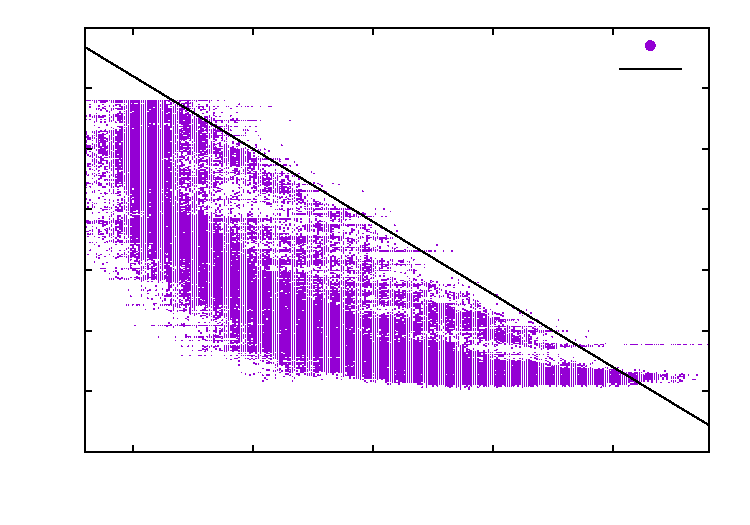
\includegraphics{lichtGoe}}%
    \gplfronttext
  \end{picture}%
\endgroup

	\caption{Alle gemessenen Intensitätwerte aus Göttingen logarithmisch aufgetragen. Des Weiteren ist die Grenzgerade, welche die mittlere Intensitätsabnahme darstellt, eingetragen.}
	\label{fig:lichtGoe}
\end{figure}
Bei den Göttingen Messungen, zeigte sich, dass der See mit vielen Schwebeteilchen durchzogen war, somit der Absorptionskoeffizient nicht nur rein vom Wasser abhängt.
Wie oben geschrieben wurde alle aufgenommenen Messwerte der Absorption gegen die Tiefe aufgetragen.
Dies ist für Göttingen in der Abbildung \ref{fig:lichtGoe} zu sehen.
Dadurch, dass alle Messwerte aufgetragen sind, ergibt sich ein linearer Zusammenhang, der proportional zum Mittelwert der gemessenen Absorption ist.
Die linearer Regression ergibt den Steigungskoeffizienten $a=(-3.3\pm0.3)\si{\per\meter}$.
Bei der Messung wurde mit einem Offset von $3.31\si{\milli\volt}$ gerechnet, da die Photodiode hier einen nicht verschwindenden Dunkelstrom hat.

\subsubsection{Northeimer Kiessee}
Bei der Messung in Northeim konnte in größeren Tiefen gemessen werden, als in Göttingen.
Somit sollten auch die Messwerte besser korrelieren.
Des Weiteren haben wir bemerkt, dass der See deutlich klarer war, als der in Göttingen, somit sollte die Absorption stärker von der des Wassers abhängen.
\begin{figure}[!h]
	\centering
	\subfigure[Alle Messwerte der Lichtabsorption in Northeim logarithmisch aufgetragen. Zu dem ist wieder die Grenzgerade eingetragen. \label{fig:lichtabs}]
   {\resizebox{0.7\linewidth}{!}{% GNUPLOT: LaTeX picture with Postscript
\begingroup
  \makeatletter
  \providecommand\color[2][]{%
    \GenericError{(gnuplot) \space\space\space\@spaces}{%
      Package color not loaded in conjunction with
      terminal option `colourtext'%
    }{See the gnuplot documentation for explanation.%
    }{Either use 'blacktext' in gnuplot or load the package
      color.sty in LaTeX.}%
    \renewcommand\color[2][]{}%
  }%
  \providecommand\includegraphics[2][]{%
    \GenericError{(gnuplot) \space\space\space\@spaces}{%
      Package graphicx or graphics not loaded%
    }{See the gnuplot documentation for explanation.%
    }{The gnuplot epslatex terminal needs graphicx.sty or graphics.sty.}%
    \renewcommand\includegraphics[2][]{}%
  }%
  \providecommand\rotatebox[2]{#2}%
  \@ifundefined{ifGPcolor}{%
    \newif\ifGPcolor
    \GPcolortrue
  }{}%
  \@ifundefined{ifGPblacktext}{%
    \newif\ifGPblacktext
    \GPblacktexttrue
  }{}%
  % define a \g@addto@macro without @ in the name:
  \let\gplgaddtomacro\g@addto@macro
  % define empty templates for all commands taking text:
  \gdef\gplbacktext{}%
  \gdef\gplfronttext{}%
  \makeatother
  \ifGPblacktext
    % no textcolor at all
    \def\colorrgb#1{}%
    \def\colorgray#1{}%
  \else
    % gray or color?
    \ifGPcolor
      \def\colorrgb#1{\color[rgb]{#1}}%
      \def\colorgray#1{\color[gray]{#1}}%
      \expandafter\def\csname LTw\endcsname{\color{white}}%
      \expandafter\def\csname LTb\endcsname{\color{black}}%
      \expandafter\def\csname LTa\endcsname{\color{black}}%
      \expandafter\def\csname LT0\endcsname{\color[rgb]{1,0,0}}%
      \expandafter\def\csname LT1\endcsname{\color[rgb]{0,1,0}}%
      \expandafter\def\csname LT2\endcsname{\color[rgb]{0,0,1}}%
      \expandafter\def\csname LT3\endcsname{\color[rgb]{1,0,1}}%
      \expandafter\def\csname LT4\endcsname{\color[rgb]{0,1,1}}%
      \expandafter\def\csname LT5\endcsname{\color[rgb]{1,1,0}}%
      \expandafter\def\csname LT6\endcsname{\color[rgb]{0,0,0}}%
      \expandafter\def\csname LT7\endcsname{\color[rgb]{1,0.3,0}}%
      \expandafter\def\csname LT8\endcsname{\color[rgb]{0.5,0.5,0.5}}%
    \else
      % gray
      \def\colorrgb#1{\color{black}}%
      \def\colorgray#1{\color[gray]{#1}}%
      \expandafter\def\csname LTw\endcsname{\color{white}}%
      \expandafter\def\csname LTb\endcsname{\color{black}}%
      \expandafter\def\csname LTa\endcsname{\color{black}}%
      \expandafter\def\csname LT0\endcsname{\color{black}}%
      \expandafter\def\csname LT1\endcsname{\color{black}}%
      \expandafter\def\csname LT2\endcsname{\color{black}}%
      \expandafter\def\csname LT3\endcsname{\color{black}}%
      \expandafter\def\csname LT4\endcsname{\color{black}}%
      \expandafter\def\csname LT5\endcsname{\color{black}}%
      \expandafter\def\csname LT6\endcsname{\color{black}}%
      \expandafter\def\csname LT7\endcsname{\color{black}}%
      \expandafter\def\csname LT8\endcsname{\color{black}}%
    \fi
  \fi
  \setlength{\unitlength}{0.0500bp}%
  \begin{picture}(7200.00,5040.00)%
    \gplgaddtomacro\gplbacktext{%
      \csname LTb\endcsname%
      \put(946,704){\makebox(0,0)[r]{\strut{}-6}}%
      \put(946,1111){\makebox(0,0)[r]{\strut{}-5.5}}%
      \put(946,1518){\makebox(0,0)[r]{\strut{}-5}}%
      \put(946,1925){\makebox(0,0)[r]{\strut{}-4.5}}%
      \put(946,2332){\makebox(0,0)[r]{\strut{}-4}}%
      \put(946,2740){\makebox(0,0)[r]{\strut{}-3.5}}%
      \put(946,3147){\makebox(0,0)[r]{\strut{}-3}}%
      \put(946,3554){\makebox(0,0)[r]{\strut{}-2.5}}%
      \put(946,3961){\makebox(0,0)[r]{\strut{}-2}}%
      \put(946,4368){\makebox(0,0)[r]{\strut{}-1.5}}%
      \put(946,4775){\makebox(0,0)[r]{\strut{}-1}}%
      \put(1227,484){\makebox(0,0){\strut{} 0}}%
      \put(1970,484){\makebox(0,0){\strut{} 1}}%
      \put(2714,484){\makebox(0,0){\strut{} 2}}%
      \put(3457,484){\makebox(0,0){\strut{} 3}}%
      \put(4201,484){\makebox(0,0){\strut{} 4}}%
      \put(4944,484){\makebox(0,0){\strut{} 5}}%
      \put(5688,484){\makebox(0,0){\strut{} 6}}%
      \put(6431,484){\makebox(0,0){\strut{} 7}}%
      \put(176,2739){\rotatebox{-270}{\makebox(0,0){\strut{}$\ln{I}$}}}%
      \put(3940,154){\makebox(0,0){\strut{}$z$ [m]}}%
    }%
    \gplgaddtomacro\gplfronttext{%
      \csname LTb\endcsname%
      \put(5816,4602){\makebox(0,0)[r]{\strut{}Messwerte}}%
      \csname LTb\endcsname%
      \put(5816,4382){\makebox(0,0)[r]{\strut{}Grenzgerade}}%
    }%
    \gplbacktext
    \put(0,0){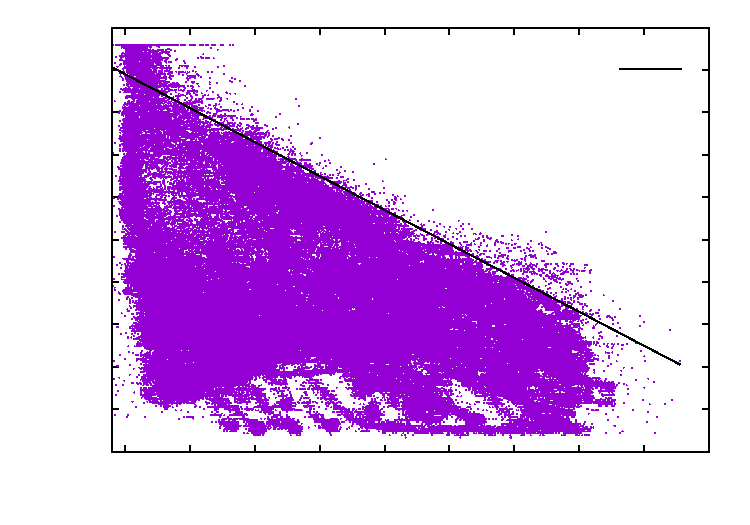
\includegraphics{licht}}%
    \gplfronttext
  \end{picture}%
\endgroup
}}
   \hfill
   \subfigure[Einzelne Messugen mit guter Korrelation.\label{fig:l1}]
   {\resizebox{.49\linewidth}{!}{% GNUPLOT: LaTeX picture with Postscript
\begingroup
  \makeatletter
  \providecommand\color[2][]{%
    \GenericError{(gnuplot) \space\space\space\@spaces}{%
      Package color not loaded in conjunction with
      terminal option `colourtext'%
    }{See the gnuplot documentation for explanation.%
    }{Either use 'blacktext' in gnuplot or load the package
      color.sty in LaTeX.}%
    \renewcommand\color[2][]{}%
  }%
  \providecommand\includegraphics[2][]{%
    \GenericError{(gnuplot) \space\space\space\@spaces}{%
      Package graphicx or graphics not loaded%
    }{See the gnuplot documentation for explanation.%
    }{The gnuplot epslatex terminal needs graphicx.sty or graphics.sty.}%
    \renewcommand\includegraphics[2][]{}%
  }%
  \providecommand\rotatebox[2]{#2}%
  \@ifundefined{ifGPcolor}{%
    \newif\ifGPcolor
    \GPcolortrue
  }{}%
  \@ifundefined{ifGPblacktext}{%
    \newif\ifGPblacktext
    \GPblacktexttrue
  }{}%
  % define a \g@addto@macro without @ in the name:
  \let\gplgaddtomacro\g@addto@macro
  % define empty templates for all commands taking text:
  \gdef\gplbacktext{}%
  \gdef\gplfronttext{}%
  \makeatother
  \ifGPblacktext
    % no textcolor at all
    \def\colorrgb#1{}%
    \def\colorgray#1{}%
  \else
    % gray or color?
    \ifGPcolor
      \def\colorrgb#1{\color[rgb]{#1}}%
      \def\colorgray#1{\color[gray]{#1}}%
      \expandafter\def\csname LTw\endcsname{\color{white}}%
      \expandafter\def\csname LTb\endcsname{\color{black}}%
      \expandafter\def\csname LTa\endcsname{\color{black}}%
      \expandafter\def\csname LT0\endcsname{\color[rgb]{1,0,0}}%
      \expandafter\def\csname LT1\endcsname{\color[rgb]{0,1,0}}%
      \expandafter\def\csname LT2\endcsname{\color[rgb]{0,0,1}}%
      \expandafter\def\csname LT3\endcsname{\color[rgb]{1,0,1}}%
      \expandafter\def\csname LT4\endcsname{\color[rgb]{0,1,1}}%
      \expandafter\def\csname LT5\endcsname{\color[rgb]{1,1,0}}%
      \expandafter\def\csname LT6\endcsname{\color[rgb]{0,0,0}}%
      \expandafter\def\csname LT7\endcsname{\color[rgb]{1,0.3,0}}%
      \expandafter\def\csname LT8\endcsname{\color[rgb]{0.5,0.5,0.5}}%
    \else
      % gray
      \def\colorrgb#1{\color{black}}%
      \def\colorgray#1{\color[gray]{#1}}%
      \expandafter\def\csname LTw\endcsname{\color{white}}%
      \expandafter\def\csname LTb\endcsname{\color{black}}%
      \expandafter\def\csname LTa\endcsname{\color{black}}%
      \expandafter\def\csname LT0\endcsname{\color{black}}%
      \expandafter\def\csname LT1\endcsname{\color{black}}%
      \expandafter\def\csname LT2\endcsname{\color{black}}%
      \expandafter\def\csname LT3\endcsname{\color{black}}%
      \expandafter\def\csname LT4\endcsname{\color{black}}%
      \expandafter\def\csname LT5\endcsname{\color{black}}%
      \expandafter\def\csname LT6\endcsname{\color{black}}%
      \expandafter\def\csname LT7\endcsname{\color{black}}%
      \expandafter\def\csname LT8\endcsname{\color{black}}%
    \fi
  \fi
    \setlength{\unitlength}{0.0500bp}%
    \ifx\gptboxheight\undefined%
      \newlength{\gptboxheight}%
      \newlength{\gptboxwidth}%
      \newsavebox{\gptboxtext}%
    \fi%
    \setlength{\fboxrule}{0.5pt}%
    \setlength{\fboxsep}{1pt}%
\begin{picture}(7200.00,5040.00)%
    \gplgaddtomacro\gplbacktext{%
      \csname LTb\endcsname%
      \put(682,704){\makebox(0,0)[r]{\strut{}$-8$}}%
      \put(682,1286){\makebox(0,0)[r]{\strut{}$-7$}}%
      \put(682,1867){\makebox(0,0)[r]{\strut{}$-6$}}%
      \put(682,2449){\makebox(0,0)[r]{\strut{}$-5$}}%
      \put(682,3030){\makebox(0,0)[r]{\strut{}$-4$}}%
      \put(682,3612){\makebox(0,0)[r]{\strut{}$-3$}}%
      \put(682,4193){\makebox(0,0)[r]{\strut{}$-2$}}%
      \put(682,4775){\makebox(0,0)[r]{\strut{}$-1$}}%
      \put(970,484){\makebox(0,0){\strut{}$0$}}%
      \put(1747,484){\makebox(0,0){\strut{}$1$}}%
      \put(2525,484){\makebox(0,0){\strut{}$2$}}%
      \put(3303,484){\makebox(0,0){\strut{}$3$}}%
      \put(4081,484){\makebox(0,0){\strut{}$4$}}%
      \put(4859,484){\makebox(0,0){\strut{}$5$}}%
      \put(5636,484){\makebox(0,0){\strut{}$6$}}%
      \put(6414,484){\makebox(0,0){\strut{}$7$}}%
    }%
    \gplgaddtomacro\gplfronttext{%
      \csname LTb\endcsname%
      \put(176,2739){\rotatebox{-270}{\makebox(0,0){\strut{}$\ln{I}$}}}%
      \put(3808,154){\makebox(0,0){\strut{}$z$ [m]}}%
      \csname LTb\endcsname%
      \put(5816,4602){\makebox(0,0)[r]{\strut{}$r=-0.96$, $a=-0.773	\pm 0.004$}}%
      \csname LTb\endcsname%
      \put(5816,4382){\makebox(0,0)[r]{\strut{}$r=-0.96$, $a=-0.501	\pm 0.003$}}%
      \csname LTb\endcsname%
      \put(5816,4162){\makebox(0,0)[r]{\strut{}$r=-0.93$, $a=-0.524	\pm 0.004$}}%
    }%
    \gplbacktext
    \put(0,0){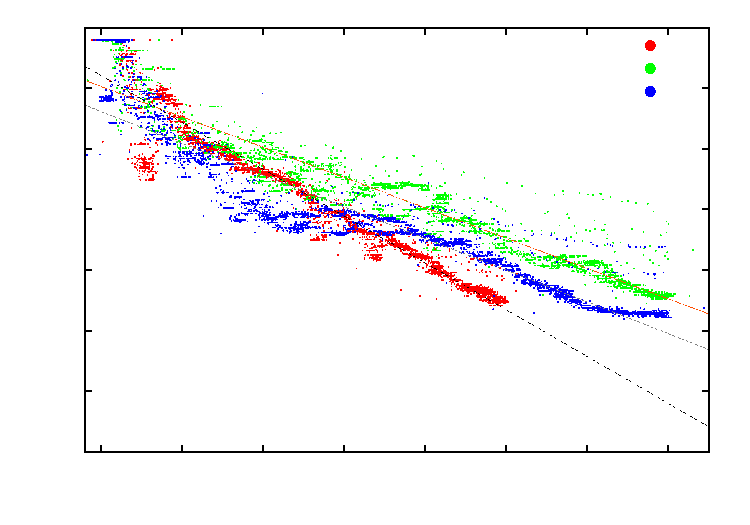
\includegraphics{l1}}%
    \gplfronttext
  \end{picture}%
\endgroup
}}
   \hfill
   \subfigure[Einzelne Messungen mit schlechte Korrelation.\label{fig:l2}]
   {\resizebox{.49\linewidth}{!}{% GNUPLOT: LaTeX picture with Postscript
\begingroup
  \makeatletter
  \providecommand\color[2][]{%
    \GenericError{(gnuplot) \space\space\space\@spaces}{%
      Package color not loaded in conjunction with
      terminal option `colourtext'%
    }{See the gnuplot documentation for explanation.%
    }{Either use 'blacktext' in gnuplot or load the package
      color.sty in LaTeX.}%
    \renewcommand\color[2][]{}%
  }%
  \providecommand\includegraphics[2][]{%
    \GenericError{(gnuplot) \space\space\space\@spaces}{%
      Package graphicx or graphics not loaded%
    }{See the gnuplot documentation for explanation.%
    }{The gnuplot epslatex terminal needs graphicx.sty or graphics.sty.}%
    \renewcommand\includegraphics[2][]{}%
  }%
  \providecommand\rotatebox[2]{#2}%
  \@ifundefined{ifGPcolor}{%
    \newif\ifGPcolor
    \GPcolortrue
  }{}%
  \@ifundefined{ifGPblacktext}{%
    \newif\ifGPblacktext
    \GPblacktexttrue
  }{}%
  % define a \g@addto@macro without @ in the name:
  \let\gplgaddtomacro\g@addto@macro
  % define empty templates for all commands taking text:
  \gdef\gplbacktext{}%
  \gdef\gplfronttext{}%
  \makeatother
  \ifGPblacktext
    % no textcolor at all
    \def\colorrgb#1{}%
    \def\colorgray#1{}%
  \else
    % gray or color?
    \ifGPcolor
      \def\colorrgb#1{\color[rgb]{#1}}%
      \def\colorgray#1{\color[gray]{#1}}%
      \expandafter\def\csname LTw\endcsname{\color{white}}%
      \expandafter\def\csname LTb\endcsname{\color{black}}%
      \expandafter\def\csname LTa\endcsname{\color{black}}%
      \expandafter\def\csname LT0\endcsname{\color[rgb]{1,0,0}}%
      \expandafter\def\csname LT1\endcsname{\color[rgb]{0,1,0}}%
      \expandafter\def\csname LT2\endcsname{\color[rgb]{0,0,1}}%
      \expandafter\def\csname LT3\endcsname{\color[rgb]{1,0,1}}%
      \expandafter\def\csname LT4\endcsname{\color[rgb]{0,1,1}}%
      \expandafter\def\csname LT5\endcsname{\color[rgb]{1,1,0}}%
      \expandafter\def\csname LT6\endcsname{\color[rgb]{0,0,0}}%
      \expandafter\def\csname LT7\endcsname{\color[rgb]{1,0.3,0}}%
      \expandafter\def\csname LT8\endcsname{\color[rgb]{0.5,0.5,0.5}}%
    \else
      % gray
      \def\colorrgb#1{\color{black}}%
      \def\colorgray#1{\color[gray]{#1}}%
      \expandafter\def\csname LTw\endcsname{\color{white}}%
      \expandafter\def\csname LTb\endcsname{\color{black}}%
      \expandafter\def\csname LTa\endcsname{\color{black}}%
      \expandafter\def\csname LT0\endcsname{\color{black}}%
      \expandafter\def\csname LT1\endcsname{\color{black}}%
      \expandafter\def\csname LT2\endcsname{\color{black}}%
      \expandafter\def\csname LT3\endcsname{\color{black}}%
      \expandafter\def\csname LT4\endcsname{\color{black}}%
      \expandafter\def\csname LT5\endcsname{\color{black}}%
      \expandafter\def\csname LT6\endcsname{\color{black}}%
      \expandafter\def\csname LT7\endcsname{\color{black}}%
      \expandafter\def\csname LT8\endcsname{\color{black}}%
    \fi
  \fi
  \setlength{\unitlength}{0.0500bp}%
  \begin{picture}(7200.00,5040.00)%
    \gplgaddtomacro\gplbacktext{%
      \csname LTb\endcsname%
      \put(946,704){\makebox(0,0)[r]{\strut{}-6}}%
      \put(946,1111){\makebox(0,0)[r]{\strut{}-5.5}}%
      \put(946,1518){\makebox(0,0)[r]{\strut{}-5}}%
      \put(946,1925){\makebox(0,0)[r]{\strut{}-4.5}}%
      \put(946,2332){\makebox(0,0)[r]{\strut{}-4}}%
      \put(946,2740){\makebox(0,0)[r]{\strut{}-3.5}}%
      \put(946,3147){\makebox(0,0)[r]{\strut{}-3}}%
      \put(946,3554){\makebox(0,0)[r]{\strut{}-2.5}}%
      \put(946,3961){\makebox(0,0)[r]{\strut{}-2}}%
      \put(946,4368){\makebox(0,0)[r]{\strut{}-1.5}}%
      \put(946,4775){\makebox(0,0)[r]{\strut{}-1}}%
      \put(1227,484){\makebox(0,0){\strut{} 0}}%
      \put(1970,484){\makebox(0,0){\strut{} 1}}%
      \put(2714,484){\makebox(0,0){\strut{} 2}}%
      \put(3457,484){\makebox(0,0){\strut{} 3}}%
      \put(4201,484){\makebox(0,0){\strut{} 4}}%
      \put(4944,484){\makebox(0,0){\strut{} 5}}%
      \put(5688,484){\makebox(0,0){\strut{} 6}}%
      \put(6431,484){\makebox(0,0){\strut{} 7}}%
      \put(176,2739){\rotatebox{-270}{\makebox(0,0){\strut{}$\ln{I}$}}}%
      \put(3940,154){\makebox(0,0){\strut{}$z$ [m]}}%
    }%
    \gplgaddtomacro\gplfronttext{%
      \csname LTb\endcsname%
      \put(5816,4602){\makebox(0,0)[r]{\strut{}$r=-0.05$}}%
      \csname LTb\endcsname%
      \put(5816,4382){\makebox(0,0)[r]{\strut{}$r=-0.59$}}%
    }%
    \gplbacktext
    \put(0,0){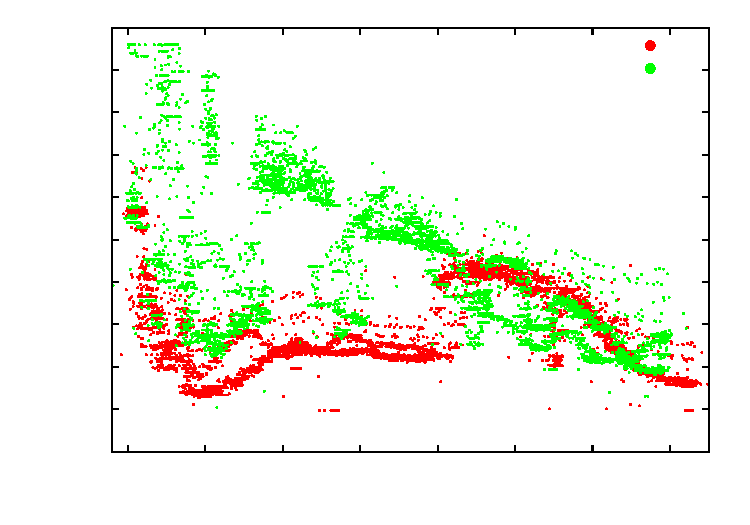
\includegraphics{l2}}%
    \gplfronttext
  \end{picture}%
\endgroup
}}
   \hfill
	\caption{Ergebnisse der Absorptionsmessung in Northeim. Es sind die Ergebnisse der Grenzgeraden und einige Korrelationen aufgetragen.}
	\label{fig:lichtNort}
\end{figure}
In Abbildung \ref{fig:lichtabs} sind wieder alle aufgenommenen Messwerte der Intensität gegen die Tiefe aufgetragen.
$a=0.40\pm0.02$.
Ebenfalls ist wieder eine linearer Regression durchgeführt worden, die den Mittelwert der Absorption zeigt, da der See wieder als homogen angenommen wird.\\%Ergebnisse
In den Abbildungen \ref{fig:l1} und \ref{fig:l2} sind jeweils gute und schlechte Korrelationen zu sehen.
Es ist gut zu erkennen, dass an einigen Stellen die Photodiode homogen beschienen wird und somit durchgehend die Absorption vom Wasser bestimmt werden konnte.
Die zeigt sich auch in den Korrelationskoeffizienten, die alle zwischen $r=0.93$ und $r=0.96$ liegen.
Die linearen Konstanten sind zwar alle etwas unterschiedliche, von $a=-0.773\pm0.004$ bis zu $-0.524\pm0.004$.
Mittelt man aber über alle Messwerte ergibt sich auf die Steigung der Geraden, wie im Gesamtplot \ref{fig:lichtabs} gezeigt.
In der schlechten Messung ist die linearer Auswertung fast nicht möglich, da die Messwerte sehr stark schwanken.
Die Korrelationskoeffizienten bestätigen dieses, da sie mit $r=-0.59$ und $r=-0.05$ sehr schlecht sind.\\
\begin{figure}[!htb]
	\centering
	\resizebox{0.7\linewidth}{!}{% GNUPLOT: LaTeX picture with Postscript
\begingroup
  \makeatletter
  \providecommand\color[2][]{%
    \GenericError{(gnuplot) \space\space\space\@spaces}{%
      Package color not loaded in conjunction with
      terminal option `colourtext'%
    }{See the gnuplot documentation for explanation.%
    }{Either use 'blacktext' in gnuplot or load the package
      color.sty in LaTeX.}%
    \renewcommand\color[2][]{}%
  }%
  \providecommand\includegraphics[2][]{%
    \GenericError{(gnuplot) \space\space\space\@spaces}{%
      Package graphicx or graphics not loaded%
    }{See the gnuplot documentation for explanation.%
    }{The gnuplot epslatex terminal needs graphicx.sty or graphics.sty.}%
    \renewcommand\includegraphics[2][]{}%
  }%
  \providecommand\rotatebox[2]{#2}%
  \@ifundefined{ifGPcolor}{%
    \newif\ifGPcolor
    \GPcolortrue
  }{}%
  \@ifundefined{ifGPblacktext}{%
    \newif\ifGPblacktext
    \GPblacktexttrue
  }{}%
  % define a \g@addto@macro without @ in the name:
  \let\gplgaddtomacro\g@addto@macro
  % define empty templates for all commands taking text:
  \gdef\gplbacktext{}%
  \gdef\gplfronttext{}%
  \makeatother
  \ifGPblacktext
    % no textcolor at all
    \def\colorrgb#1{}%
    \def\colorgray#1{}%
  \else
    % gray or color?
    \ifGPcolor
      \def\colorrgb#1{\color[rgb]{#1}}%
      \def\colorgray#1{\color[gray]{#1}}%
      \expandafter\def\csname LTw\endcsname{\color{white}}%
      \expandafter\def\csname LTb\endcsname{\color{black}}%
      \expandafter\def\csname LTa\endcsname{\color{black}}%
      \expandafter\def\csname LT0\endcsname{\color[rgb]{1,0,0}}%
      \expandafter\def\csname LT1\endcsname{\color[rgb]{0,1,0}}%
      \expandafter\def\csname LT2\endcsname{\color[rgb]{0,0,1}}%
      \expandafter\def\csname LT3\endcsname{\color[rgb]{1,0,1}}%
      \expandafter\def\csname LT4\endcsname{\color[rgb]{0,1,1}}%
      \expandafter\def\csname LT5\endcsname{\color[rgb]{1,1,0}}%
      \expandafter\def\csname LT6\endcsname{\color[rgb]{0,0,0}}%
      \expandafter\def\csname LT7\endcsname{\color[rgb]{1,0.3,0}}%
      \expandafter\def\csname LT8\endcsname{\color[rgb]{0.5,0.5,0.5}}%
    \else
      % gray
      \def\colorrgb#1{\color{black}}%
      \def\colorgray#1{\color[gray]{#1}}%
      \expandafter\def\csname LTw\endcsname{\color{white}}%
      \expandafter\def\csname LTb\endcsname{\color{black}}%
      \expandafter\def\csname LTa\endcsname{\color{black}}%
      \expandafter\def\csname LT0\endcsname{\color{black}}%
      \expandafter\def\csname LT1\endcsname{\color{black}}%
      \expandafter\def\csname LT2\endcsname{\color{black}}%
      \expandafter\def\csname LT3\endcsname{\color{black}}%
      \expandafter\def\csname LT4\endcsname{\color{black}}%
      \expandafter\def\csname LT5\endcsname{\color{black}}%
      \expandafter\def\csname LT6\endcsname{\color{black}}%
      \expandafter\def\csname LT7\endcsname{\color{black}}%
      \expandafter\def\csname LT8\endcsname{\color{black}}%
    \fi
  \fi
  \setlength{\unitlength}{0.0500bp}%
  \begin{picture}(7200.00,5040.00)%
    \gplgaddtomacro\gplbacktext{%
      \csname LTb\endcsname%
      \put(1078,704){\makebox(0,0)[r]{\strut{}-0.02}}%
      \put(1078,1518){\makebox(0,0)[r]{\strut{}-0.01}}%
      \put(1078,2332){\makebox(0,0)[r]{\strut{} 0}}%
      \put(1078,3147){\makebox(0,0)[r]{\strut{} 0.01}}%
      \put(1078,3961){\makebox(0,0)[r]{\strut{} 0.02}}%
      \put(1078,4775){\makebox(0,0)[r]{\strut{} 0.03}}%
      \put(1355,484){\makebox(0,0){\strut{} 0}}%
      \put(2082,484){\makebox(0,0){\strut{} 1}}%
      \put(2808,484){\makebox(0,0){\strut{} 2}}%
      \put(3534,484){\makebox(0,0){\strut{} 3}}%
      \put(4261,484){\makebox(0,0){\strut{} 4}}%
      \put(4987,484){\makebox(0,0){\strut{} 5}}%
      \put(5713,484){\makebox(0,0){\strut{} 6}}%
      \put(6440,484){\makebox(0,0){\strut{} 7}}%
      \put(176,2739){\rotatebox{-270}{\makebox(0,0){\strut{}$\Delta U \propto\Delta I$ [V]}}}%
      \put(4006,154){\makebox(0,0){\strut{}$z$ [m]}}%
    }%
    \gplgaddtomacro\gplfronttext{%
      \csname LTb\endcsname%
      \put(5816,4602){\makebox(0,0)[r]{\strut{}blaue LED}}%
      \csname LTb\endcsname%
      \put(5816,4382){\makebox(0,0)[r]{\strut{}IR-LED}}%
    }%
    \gplbacktext
    \put(0,0){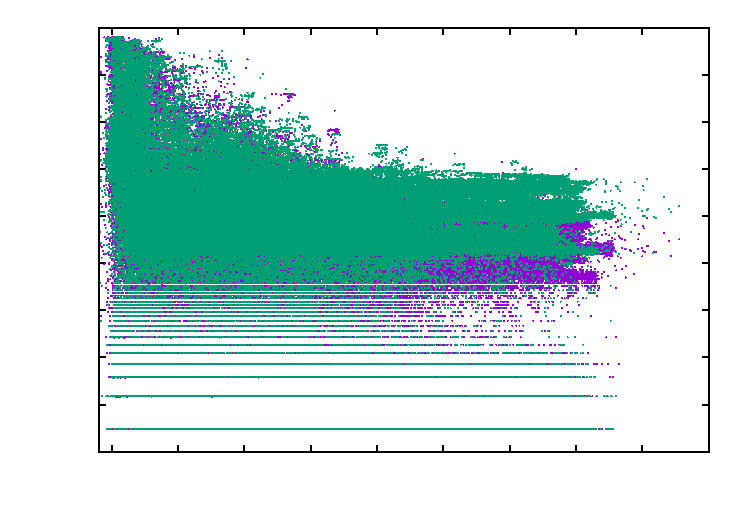
\includegraphics{led}}%
    \gplfronttext
  \end{picture}%
\endgroup
}
	\caption{Intensität der einzelnen LEDs (Infrarot und Blau) in Differenz zur Sonnenintensität aufgetragen für die Northeimer Messung.}
	\label{fig:led}
\end{figure}
In der Abbildung \ref{fig:led} sind die gemessenen Intensitäten der LEDs gegen die Tiefe aufgetragen.
Hierzu wurden jeweils die Intensitäten bei abgeschalteten LEDs von den jeweiligen Werten bei angeschalteten LEDs subtrahiert.
Dies soll zu dem das Rauschen der Sonnenintensität reduzieren.%diesen Punkt kann an gut diskutieren
Das Ergebnis zeigt eine Konstante, die aber für die beiden LEDs verschieden sind.
Des Weiteren ist die, wie oben beschriebene Streuungen auf den ersten Metern immer noch gut zu erkennen.
Da die Werte konstant gegen die Tiefe sind berechnen wir den Mittelwert aus den jeweiligen Intensitäten.
Für die blaue LED ergibt sich eine mittlere Intensität von $I_\text{blau}=(3.1\pm2.7)\si{\volt}$ und für infrarote eine mittlere Intensität von $I_\text{IR}=(5.9\pm3.7)\si{\volt}$.
Die größer der Fehler von bis zu 88\% ergeben sich aus den starken Streuungen der Messwerte.
Die Fehler bilden sich jeweils aus der Standardabweichung.
Die Infrarote LED hat somit eine etwa doppelt so hohe Intensität, wie die Blaue LED.

\subsection{Gemessenes Abstandsgesetz}
Da nun die Sendeleistung nicht ausreichte, um die Anordnung der Piezokristalle tatsächlich als Echolot zu verwenden haben wir nur die Abstandsabhängigkeit der Schallintensität näher untersucht. 
Dies wurde zunächst mit der Motivation durchgeführt eine mit der vorgegebenen Sendeleistung maximale Reichweite zu ermitteln. Als klar wurde, dass diese nicht ausreichen wird haben wir
die Abnahme der Amplitude weiter untersucht.

Zu diesem Zweck haben wir Sender und Empfänger parallel zueinander ausgerichtet und den Abstand mit einer Skala gemessen. Um dann die Amplitude bei einer bestimmten Entfernung abzulesen, haben wir ein
ein Oszilloskop als Empfänger verwendet.

Wir haben hierfür drei Messreihen durchgeführt und anschließend wurde für jede Entfernung der Mittelwert mit Standardabweichung berechnet. In Grafik \ref{fig:schall} ist das Messergebnis zu sehen, wobei wir die relative Amplitude $\frac{A}{A_0}$ berechnet haben.

\begin{figure}[h]
	\centering
	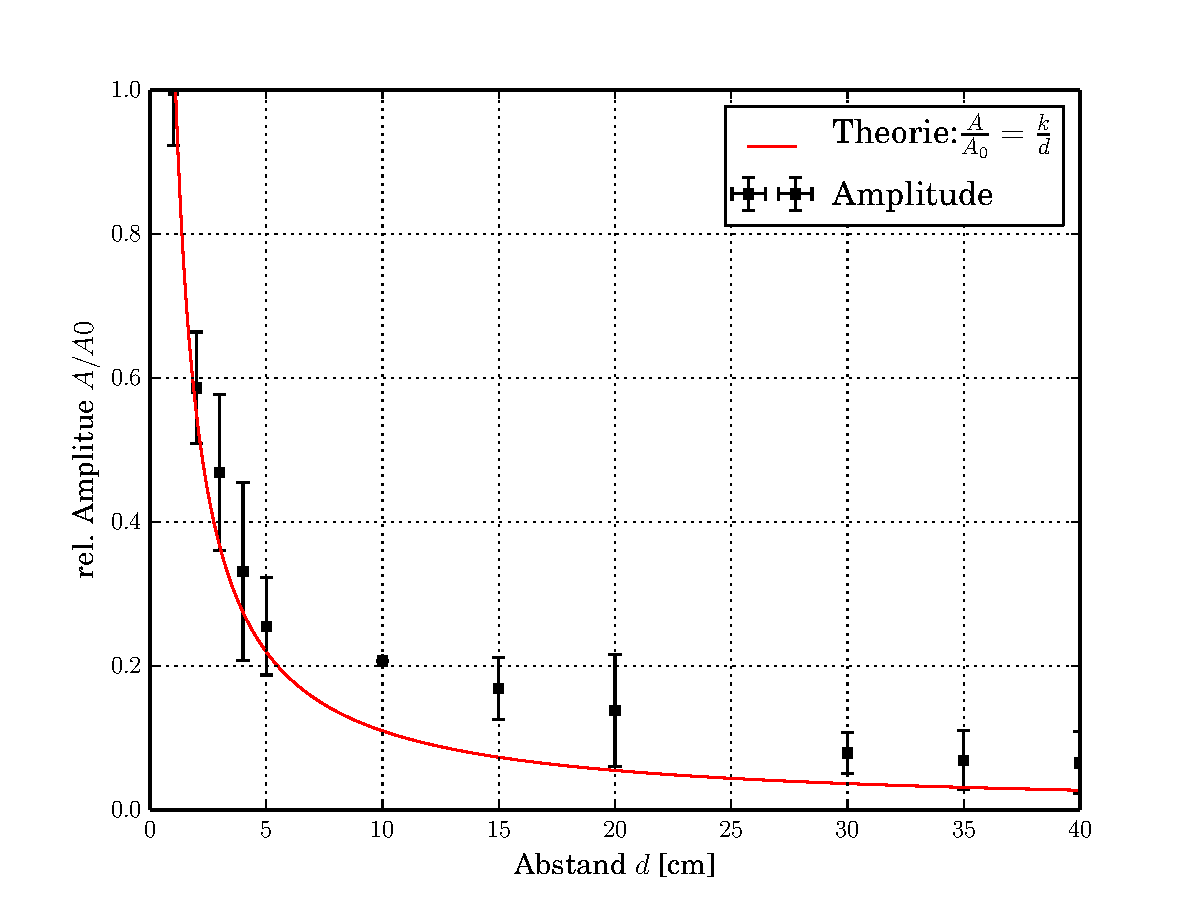
\includegraphics[width=0.8\textwidth]{schall.pdf}
	\caption{Relative Amplitude des Echolotes wurde aufgetragen gegen den Abstand $d$. Zudem wurde eine $\chi^2$ Anpassung an die Messdaten durchgeführt.}
	\label{fig:schall}
\end{figure}

Zudem wurde eine $\chi^2$ Anpassung an die berechneten Mittelwerte durchgeführt, wobei hier die in der Theorie vorgestellte $\frac{1}{d}$ - Abhängigkeit angenommen wurde, sprich die mit dem Oszilloskop gemessene Amplitude sich wie die Abstandsabhängigkeit des Schalldrucks verhält.
Dies erscheint sinnvoll, denn entscheidend für die angezeigte Amplitude ist, welche Beschleunigungen auf den Empfänger wirken.
Diese wiederum entsprechen Druckschwankungen.

Die eingezeichneten Fehlerbalken ergeben sich nur aus der statistischen Standardabweichung da diese die abgeschätzten Fehler von 0.1\% Amplitude zu klein sind. Diese Abhängigkeit war auch hier recht gut gegeben, wie man in dem Plot erkennen kann. 
Man kann gut sehen, dass die Amplitude nach gerade einmal circa 2.5\si{\centi\meter} auf unter die Hälfte abgefallen ist. Bei einer Entfernung von 40\si{\centi\meter} ist dann nur noch gut 5 $\%$ vorhanden. Es wird also sehr deutlich, dass die Sendeleistung nicht ausreichen würde für die geplanten Versuche, denn innerhalb eines homogenen Mediums liegt stets eine $\frac{1}{d}$ -Abhängigkeit vor (siehe Abschnitt \ref{sec:abs}). 



\section{Diskussion}
\label{sec:diskussion}

\subsection{Referenzspannung des ADC}
\label{sec:diskreffADC}
Für den ADC wurde die Interne Referenzspannung des Controllers verwendet.
Diese ist aber durch den normalen Betrieb des Controllers ein klein wenig verrauscht, das sogenannte Rippling, somit auch die ADC Werte.
Dies hat eine Größenordnung von etwa 5\si{\milli\volt}, sprich 1\% der Maximalspannung und ist in allen Datensätzen zu sehen.\\
Um diesen Fehler zu beheben bzw. zu verringern ist es nötig eine konstante Referenzspannung zu verwenden.
Das Board hat einen nach außen geführten Pin für die Referenzspannung.
Nun ist es nötig entweder die 3.3\si{\volt} des Boards zu nehmen und das Rippling zu vermindern, oder eine eigene lastfreie Spannungsquelle zu bauen.
Zu den muss ein Tiefpassfilter mithilfe einer Drosselspule in Reihe geschaltet werden um das durch die Elektronik induzierte Rauschen zu unterdrücken.
Mit dieses Methoden könnte das Rippling auf etwa 0.1\% der Maximalspannung gedrückt werden.

\subsection{Druck}
Zunächst kauften wir einen Drucksensor, der keine Eichkurve hatte.
Er bestand aus zwei leitenden Lagen und je größer der auf ihn ausgeübte Druck gewesen wäre, desto größer ist die Kontaktfläche und damit desto kleiner ist der Widerstand.
Allerdings ist ein kleines Loch in der Kammer, damit die Luft entweichen kann.
Da durch dieses Wasser hineinlaufen könnte, welches einen Kurzschluss verursacht, konnten wir diesen Sensor nicht verwenden.

Daraufhin bekamen wir einen Sensor der Geophysik.
Dieser wird über eine externe Schaltung betrieben und wurde deshalb nicht von den Spannungsschwankungen des Boards direkt beeinflusst.
Der größte Fehler bei der Kopplung von Druckplatine und Datenlogger bestand noch in der Testphase darin, dass nicht, wie im Kapitel \ref{sec:durchdruck} aufgeführt, die Massen der beiden Platinen gekoppelt waren, obwohl eine eigenständige Leitung für das Massesignal verwendet wurde.
Fehlerhaft war hier nicht die Verbindung der Platinen, sondern die boardinterne Masseverteilung.
Anscheinend waren die veschiedenen Massepins nicht alle miteinander verbunden.
Dies kann an einer fehlerhaften Lötstelle oder einer fehlerhaften Leitung liegen.
In unserem Fall wurde des Problem behoben, in dem wir alle Masse zudem extern noch ein weiteres Mal gekoppelt haben.\\
Allerdings wirkte das Rippling der ADCwerte, wie in Kapitel \ref{sec:diskreffADC} beschrieben, sich auch auf die Auswertung des Drucks aus.
Des Weiteren zeigte sich in der Auswertung, dass die Steigung des Druck unterschätzt wurde.
Die Tiefe war um fast 10\% zu klein.
Aus diesem Grund haben wir den Korrekturfaktor von 1.1 verwendet.
Mit diesem Faktor sind die Tiefenwerte, wie im Kapitel \ref{sec:ausdruck} beschrieben, mit den über die Markierungen am Kabel vergleichbar gewesen.

\subsection{Echolot}
Die Idee des Echolots konnte nicht vollständig umgesetzt werden, da das Signal nicht stark genug war, um bis in eine Tiefe von etwa 6\si{\meter} einzudringen und reflektiert zu werden.
Um in diese Vordringen zu können müsste mehr Schalldruck erzeugt werden und dazu ist eine größere physische Ausdehnung des Kristalls nötig.
Dies kann entweder durch das Verwenden von einer höheren Spannung am Sender oder durch das Verwenden einer H-Brücke getan werden.
Letzteres sorgt für das Verwenden von $\pm24\si{\volt}$, welches zur doppelten physischen Ausdehnung des Kristalls führt.
Dies kann weiterhin verstärkt werden, in dem bis zu 48\si{\volt} angelegt werden.
Der Nachteil der H-Brücke ist, dass bei jedem Umschalten die Schaltung kurzgeschlossen wird, was unterbunden werden muss, da die MOSFET-Transistoren mit einer Frequenz von 40\si{\kilo\hertz} versorgt werden und dies zu einem hohen Leckstrom führt, der die Bauteile beschädigen kann.
Desweiteren erhitzen sich die Bauteile bei diesen Spannungen schnell und es müssen Kühlkörper oder eine aktive Kühlung verwendet werden.\\
Wir haben dennoch ein paar Testdaten aufnehmen und auswerten können.
%hie noch das Ergebnis der Auswertung diskutieren.
Dieser Teil des Projektes ist auch für weitere Praktika interessant, da diese Methode kommerziell häufig eingesetzt wird und auch in der Wissenschaft zur Bodenanalyse verwendet werden kann.
Die Probleme, die gelöst werden müssen, sind die Spannungsverorgung und ein funktionsfähiger Filteralgorythmuss zur Rauschreduktion.

\subsection{Ortsbestimmung}
Bei der ersten Messung haben wir den Ort mit einem Geodimeter bestimmt.
Problematisch war hierbei, dass das Boot mit dem Reflektor relativ stark geschwankt hat.
Dies führte gerade bei Messungen, wo das Boot dicht am Geodimeter war dazu, dass die Aufnahme der Position erschwert wurde.
An einer Stelle konnten wir den Messstab in über 5 min nicht ruhig genug halten, so dass wir schließlich die Position nicht aufnahmen.
Generell war es ein Problem, dass wir nur zwei Leute auf dem Boot hatten: einen Ruderer, der während der Messung den Stab hochgehalten hat und einen, der sich um die Sonde kümmerte.
Dies führte dazu, dass häufig der für den Retroreflektor zuständige diesen zu schräg hielt, so dass die Spiegelfläche nicht sichtbar war.
Da wir bei der Messung die Funkgeräte vergessen hatten, mussten wir uns mit Handzeichen verständigen.
Dies stellte selbst am Göttinger Kiessee an den entferntesten Messpunkten eine Herausforderung dar, so dass dort das Boot-Team häufig unnötig lange an einem Ort blieb, da sie die Bestätigung nicht sahen.

Außerdem behindert am Northeimer See eine Insel ein Großteil des Blickfelds, so dass das Geodimeter keinen guten Standpunkt gehabt hätte.

Es stellte sich bei den Messungen heraus, dass die Genauigkeit des Geodimeters keine Rolle spielte, da das Boot von Wind und Strömung während der Messung sehr stark abgetrieben wurde und somit mit einem Fehler von etwa $\pm5\si{\meter}$ gerechnet werden muss.
Daher setzten wir bei der zweiten Messung unsere erste Idee um, die Position über GPS zu erfassen, welche wir wegen der vermeintlich schlechten Auflösung von 5-10m verwarfen.
Somit sind beide Methoden gleich gut und bei der Messung, wie im Kapitel \ref{sec:ausort} bereits dargestellt, stellte sich zu dem heraus, dass das GPS von Garmin$^\copyright$ eine Genauigkeit von bis zu $\pm3\si{\meter}$ hatte.
Die ist eine Verbesserung von 40\% in Bezug auf die vorher Möglichen $\pm5\si{\meter}$.
Zu dem waren nun die Position in der selben Datei gespeichert, wie die Messdaten auch.
Dies machte ein sonnst notwendiges Sortieren der Dateien nach Ort und Zeit unnötig.

\subsection{Temperatur}
\label{sec:DiskTemp}
Bei der zweiten Messung zeigte sich in den Daten, wie im Kapitel \ref{sec:austempnortheim} beschrieben, dass die Werte der Temperatur augenscheinlich gleichzeitig drei verschiedene Werte annehmen.
Bei genauerer Betrachtung der Messwerte fällt jedoch auf, wie in Abb. \ref{fig:tempSprung} zu erkennen, dass jeweils ungefähr 10 Messwerte auf einem niedrigen, dann auf einem mittleren, erneut auf einem niedrigen und dann wieder auf einem hohen Niveau liegen.
Dies entspricht der Frequenz, mit der wir die LEDs geschaltet haben (keine LED, blaue LED, keine LED, IR-LED).
Für beide Messungen benutzten wir den Micro-Controller als Spannungsquelle.
Dieser ist für Ströme von bis zu 350mA ausgelegt.
Augenscheinlich haben da die etwa 30\si{\milli\ampere}, welche die LEDs benötigten, die Stromzufuhr des Pt1000 so stark beeinflusst, dass die aufgenommenen Messwerte Temperatursprünge von bis zu $4\si{\celsius}$ aufweisen, was bei angenommenen $21\si{\celsius}$ zu einem Fehler von 20\% führt.
Dies liegt vermutlich daran, dass der boardinterne Spannungsregler mit dem schnelle Spannungsschwankungen nicht zurecht kam und einige Zeit gebraucht hat, um den Spannungswert zu regeln.
Somit lagen verschiedene Spannungen am Vorwiderstand des Pt1000 an und führte trotz seiner Größe von $19200\si{\ohm}$ zu stark spürbaren Stromschwankungen am Pt1000.\\
Glücklicherweise sind die Daten so verteilt, dass nur etwa 50\% Fehlerhaft sind und diese nur gefiltert werden mussten.

\begin{figure}[h]
	\centering
	% GNUPLOT: LaTeX picture with Postscript
\begingroup
  \makeatletter
  \providecommand\color[2][]{%
    \GenericError{(gnuplot) \space\space\space\@spaces}{%
      Package color not loaded in conjunction with
      terminal option `colourtext'%
    }{See the gnuplot documentation for explanation.%
    }{Either use 'blacktext' in gnuplot or load the package
      color.sty in LaTeX.}%
    \renewcommand\color[2][]{}%
  }%
  \providecommand\includegraphics[2][]{%
    \GenericError{(gnuplot) \space\space\space\@spaces}{%
      Package graphicx or graphics not loaded%
    }{See the gnuplot documentation for explanation.%
    }{The gnuplot epslatex terminal needs graphicx.sty or graphics.sty.}%
    \renewcommand\includegraphics[2][]{}%
  }%
  \providecommand\rotatebox[2]{#2}%
  \@ifundefined{ifGPcolor}{%
    \newif\ifGPcolor
    \GPcolorfalse
  }{}%
  \@ifundefined{ifGPblacktext}{%
    \newif\ifGPblacktext
    \GPblacktexttrue
  }{}%
  % define a \g@addto@macro without @ in the name:
  \let\gplgaddtomacro\g@addto@macro
  % define empty templates for all commands taking text:
  \gdef\gplbacktext{}%
  \gdef\gplfronttext{}%
  \makeatother
  \ifGPblacktext
    % no textcolor at all
    \def\colorrgb#1{}%
    \def\colorgray#1{}%
  \else
    % gray or color?
    \ifGPcolor
      \def\colorrgb#1{\color[rgb]{#1}}%
      \def\colorgray#1{\color[gray]{#1}}%
      \expandafter\def\csname LTw\endcsname{\color{white}}%
      \expandafter\def\csname LTb\endcsname{\color{black}}%
      \expandafter\def\csname LTa\endcsname{\color{black}}%
      \expandafter\def\csname LT0\endcsname{\color[rgb]{1,0,0}}%
      \expandafter\def\csname LT1\endcsname{\color[rgb]{0,1,0}}%
      \expandafter\def\csname LT2\endcsname{\color[rgb]{0,0,1}}%
      \expandafter\def\csname LT3\endcsname{\color[rgb]{1,0,1}}%
      \expandafter\def\csname LT4\endcsname{\color[rgb]{0,1,1}}%
      \expandafter\def\csname LT5\endcsname{\color[rgb]{1,1,0}}%
      \expandafter\def\csname LT6\endcsname{\color[rgb]{0,0,0}}%
      \expandafter\def\csname LT7\endcsname{\color[rgb]{1,0.3,0}}%
      \expandafter\def\csname LT8\endcsname{\color[rgb]{0.5,0.5,0.5}}%
    \else
      % gray
      \def\colorrgb#1{\color{black}}%
      \def\colorgray#1{\color[gray]{#1}}%
      \expandafter\def\csname LTw\endcsname{\color{white}}%
      \expandafter\def\csname LTb\endcsname{\color{black}}%
      \expandafter\def\csname LTa\endcsname{\color{black}}%
      \expandafter\def\csname LT0\endcsname{\color{black}}%
      \expandafter\def\csname LT1\endcsname{\color{black}}%
      \expandafter\def\csname LT2\endcsname{\color{black}}%
      \expandafter\def\csname LT3\endcsname{\color{black}}%
      \expandafter\def\csname LT4\endcsname{\color{black}}%
      \expandafter\def\csname LT5\endcsname{\color{black}}%
      \expandafter\def\csname LT6\endcsname{\color{black}}%
      \expandafter\def\csname LT7\endcsname{\color{black}}%
      \expandafter\def\csname LT8\endcsname{\color{black}}%
    \fi
  \fi
    \setlength{\unitlength}{0.0500bp}%
    \ifx\gptboxheight\undefined%
      \newlength{\gptboxheight}%
      \newlength{\gptboxwidth}%
      \newsavebox{\gptboxtext}%
    \fi%
    \setlength{\fboxrule}{0.5pt}%
    \setlength{\fboxsep}{1pt}%
\begin{picture}(7200.00,5040.00)%
    \gplgaddtomacro\gplbacktext{%
      \csname LTb\endcsname%
      \put(682,1126){\makebox(0,0)[r]{\strut{}$18$}}%
      \put(682,1886){\makebox(0,0)[r]{\strut{}$19$}}%
      \put(682,2647){\makebox(0,0)[r]{\strut{}$20$}}%
      \put(682,3407){\makebox(0,0)[r]{\strut{}$21$}}%
      \put(682,4168){\makebox(0,0)[r]{\strut{}$22$}}%
      \put(1738,484){\makebox(0,0){\strut{}$3300$}}%
      \put(2925,484){\makebox(0,0){\strut{}$3320$}}%
      \put(4112,484){\makebox(0,0){\strut{}$3340$}}%
      \put(5300,484){\makebox(0,0){\strut{}$3360$}}%
      \put(6487,484){\makebox(0,0){\strut{}$3380$}}%
    }%
    \gplgaddtomacro\gplfronttext{%
      \csname LTb\endcsname%
      \put(176,2739){\rotatebox{-270}{\makebox(0,0){\strut{}$^\circ$ C}}}%
      \put(3808,154){\makebox(0,0){\strut{}Messpunkt}}%
      \csname LTb\endcsname%
      \put(5816,4602){\makebox(0,0)[r]{\strut{}Temperatur}}%
    }%
    \gplbacktext
    \put(0,0){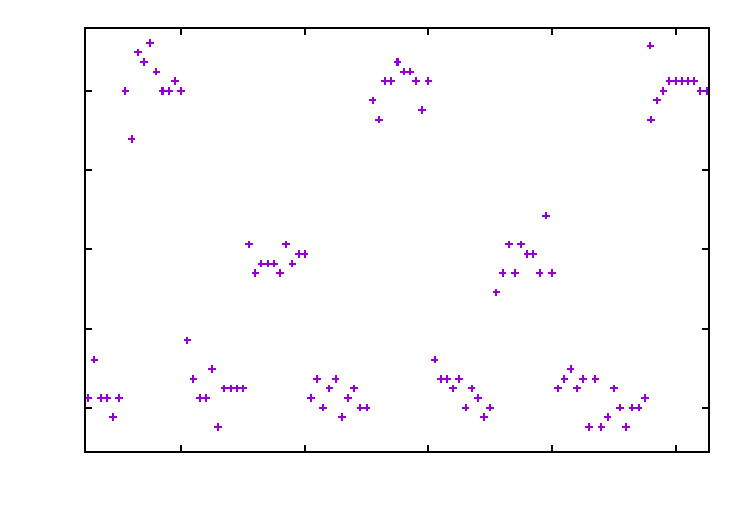
\includegraphics{tempSprung}}%
    \gplfronttext
  \end{picture}%
\endgroup

	\caption{Vergrößerte Darstellung einer Temperaturkurve. Es ist gut das Rippling in den einzelnen Blöcken und die Verschiebung der Blöcke zu sehen.}
	\label{fig:tempSprung}
\end{figure}

\subsection{Absorption}
Bei der Messung der Absorption stellte sich sehr schnell heraus, dass die Daten stark verrauscht sind, besonders an der Oberfläche des Wassers.
Dies liegt wahrscheinlich daran, dass durch die Bewegung der Wasseroberfläche das Sonnenlicht besser und schlechter Reflektiert wird.
Um dieses hochfrequente Rauschen zu unterdrücken kann der Strom der Photodiode zusätzlich noch durch einen Tiefpassfilter geleitet werden.
Hierzu müsste nur eine Drosselspule in Reihe mit der Photodiode und dem ADC geschaltet werden.
Somit werden nur die niederfrequenten Änderungen des Photostroms aufgezeichnet.\\
Desweiteren waren die beide LEDs zur Messung der Absorption in verschiedenen Spektren nicht nah genug an der Photodiode, um eine signifikate Änderung an den Werten zu führen, die nicht im Rauschen untergeht.
Ebenfalls wurde bei der Wahl der Diode nicht darauf geachtet, dass diese eine unterschiedliche Aufnahmecharakteristik für die verwendeten Wellenlängen hat.
Laut Datenblatt \cite[20]{PHOTODatenblatt} liegt der Unterschied in der Effizienz zwischen den beiden Wellenlängen bei 40\%, was sich auch in der Auswertung bemerkbar machte.\\
Die Auswertung zeigte, dass die Ergebnisse der LED Auswertung trotz der Subtraktionsmethode noch stark Rausht.
Dies zeigt sich in den großen Fehlern von bis zu 88\% in der Standartabweichung.
Desweiteren sind die mittleren Intensitäten der einzelnen LEDs auch sehr klein, da sie nur in 1\% des Messbereiches liegen.


\subsection{Messprobleme und verworfene Ideen}
Unsere erste Idee war die, ein ferngesteuertes U-Boot zu bauen, was die Sensoren an Bord hat und ansatzweise autonom den See abrastert.
Dies stellte sich jedoch sehr schnell als nicht durchführbar heraus, da es keine geeigneten Modellbauten gab und da die komplette Technik mit Stromversorgung unter Wasser luftdicht sein müsste.
Zu dem war der Bau eines eigenen Modells zu Zeitaufwändig für die vorhandene Zeit.
Daher kamen wir auf die Idee, eine ferngesteuerte Plattform zu bauen, welche die Sonden mit einer Winde ferngesteuert herunterlässt.
Dies verwarfen wir jedoch auch sehr schnell, da die Fernsteuertechnik einen großen Teil unserer Arbeit ausgemacht hätte, was wissenschaftlich wenig interessant ist.
Auch hätten wir Probleme bekommen, falls sich zum Beispiel die Sensoren in Wasserpflanzen verfangen.

So entschieden wir uns für die simplere Umsetzung, ein Ruderboot zu nehmen und die Stromversorgung, sowie die Datenverarbeitung im Boot zu betreiben und nur die Sensoren an den Kabeln herunter zu lassen.
Dies sollte zunächst mithilfe eines Datenloggers der Goephysik arbeiten, dieser nimmt allerdings nur alle 2\si{\second} einen Wert auf.
Dies ist für unsere kleinen Messdauern zu wenig und hätte zu sehr langen Messungen geführt.
Gelöst wurde das Problem mit dem Bau eines eigenen Datenloggers, mit dem wir dann 100 Messwerte pro Sekunden aufnehmen und diese auch gleich betrachten konnten.


Wir hatten zunächst noch vor, weitere Sensoren zu verwenden:
\begin{itemize}
	\item \textit{el. Leitfähigkeit}: Funktionierte nicht, da wir dafür Wechselspannungen mit mindestens 50V benötigt hätten.
		Dies wäre notwendig, da sich sonst an den Elektroden durch Elektrolyse Salze angelagert hätten, welche für eine höhere gemessene Leitfähigkeit gesorgt hätten.
		Die Leitfähigkeit alleine ist kein Maß für den Salzgehalt, der auch noch von anderen Größen maßgeblich beeinflusst wird.
		So konnten wir den Sensor, welchen Jan bereits besorgt hatte, nicht einsetzen.
	\item \textit{pH-Wert}: Der pH-Wert wäre auch eine interessante Messgröße gewesen.
		Allerdings wäre zur Kalibrierung mindestens eine Pufferlösung notwendig gewesen.
		Ausschlaggebend war, dass wir zu den preislich akzeptablen Sensoren keine vernünftigen Datenkurven finden konnten, da diese augenscheinlich nur für fertige Geräte ausgelegt sind.
\end{itemize}

\newpage
\printbibliography[heading=bibintoc]
%\bibliography{literatur}
%\bibliographystyle{babalpha}
\newpage


\appendix
\pagenumbering{Roman}
\setcounter{page}{1}
\setcounter{footnote}{0}
\section{Anhang}

\subsection{Schaltpläne}
\begin{figure}[!h]
\centering
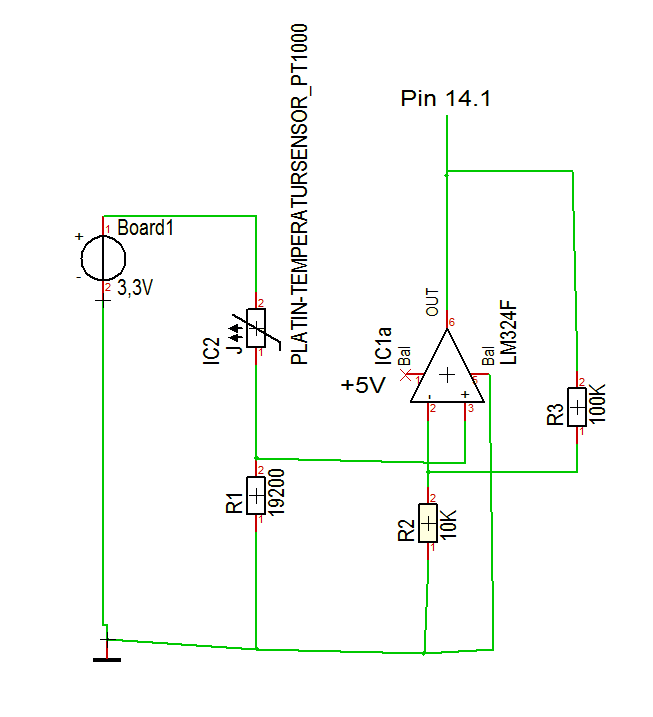
\includegraphics[width=0.5\textwidth]{Fotos/PT1000Schaltung.png}
\caption{Beschaltung des Pt1000 Temperaturwiderstandes mit Vorwiderstand und Verstärkerschltung. Die Spannungsversorgung, genau wie die Masseanbindung wird vom Board geregelt.}
\label{fig:PT1000Schaltung}
\end{figure}
\begin{figure}[!h]
\centering
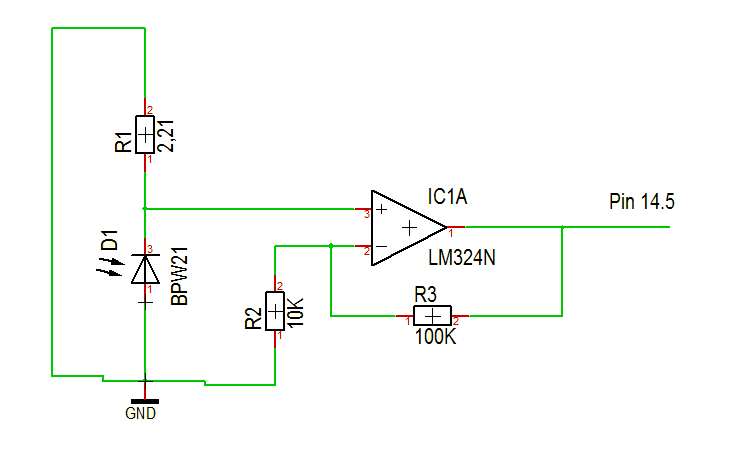
\includegraphics[width=0.5\textwidth]{Fotos/PhotodiodeSchaltung.png}
\caption{Beschaltung der Photodiode mit Widerstand und Verstärkerachaltung. Die Photodiode dient als Stromquelle und der Widerstand dient als Übersetzung in eine Spannung. Um die wenigen Millivolt detektierbar zu machen, wird ein Verstärker, wie beim Temperaturwiderstand verwerdet.}
\label{fig:PhotodiodeSchaltung}
\end{figure}
\begin{figure}[!h]
\centering
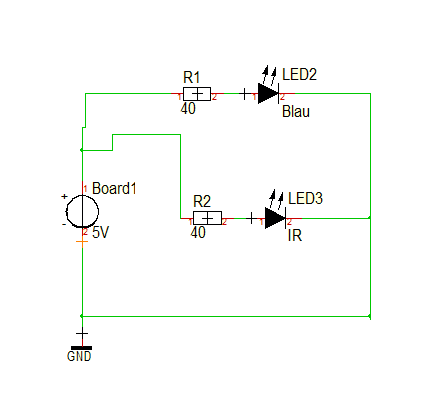
\includegraphics[width=0.6\textwidth]{Fotos/LEDSchaltung.png}
\caption{Ersatzschaltbild der LEDs für die Messung der Absorption. Die Spannung wird vom Board bereitgestellt. Auf dem Board werden die LEDs durch bipolare Transistoren geschaltet und über den selben Widerstand versorgt, da sie nie zur selben Zeit eingeschaltet sind.}
\label{fig:LEDSchaltung}
\end{figure}
\begin{figure}[!h]
\centering
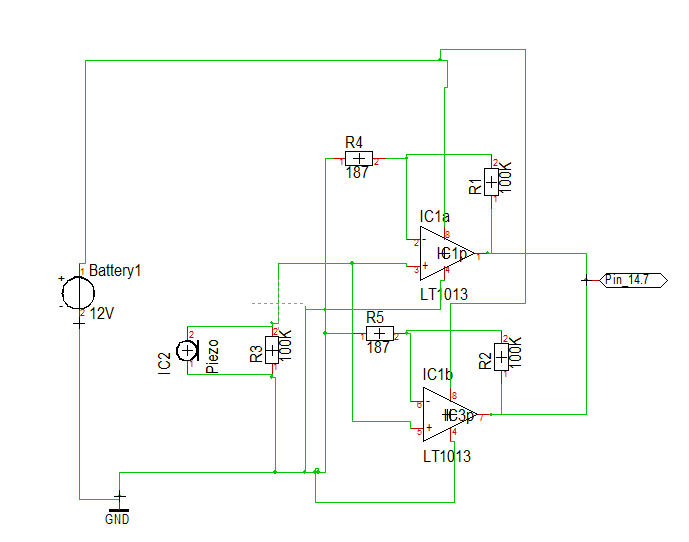
\includegraphics[width=0.6\textwidth]{Fotos/Echoverstaerker.png}
\caption{Schaltung für den Empfängerpiezo, mit eigener Spannungsquelle und zwei Verstärkern zur Rauschverminderung. Die Spannung wird durch externe Akkus gewährleistet und der Piezo wird als Spannungsquelle geschaltet.}
\label{fig:Echoverstaerker}
\end{figure}



%\begin{figure}[h]
%	\centering
%	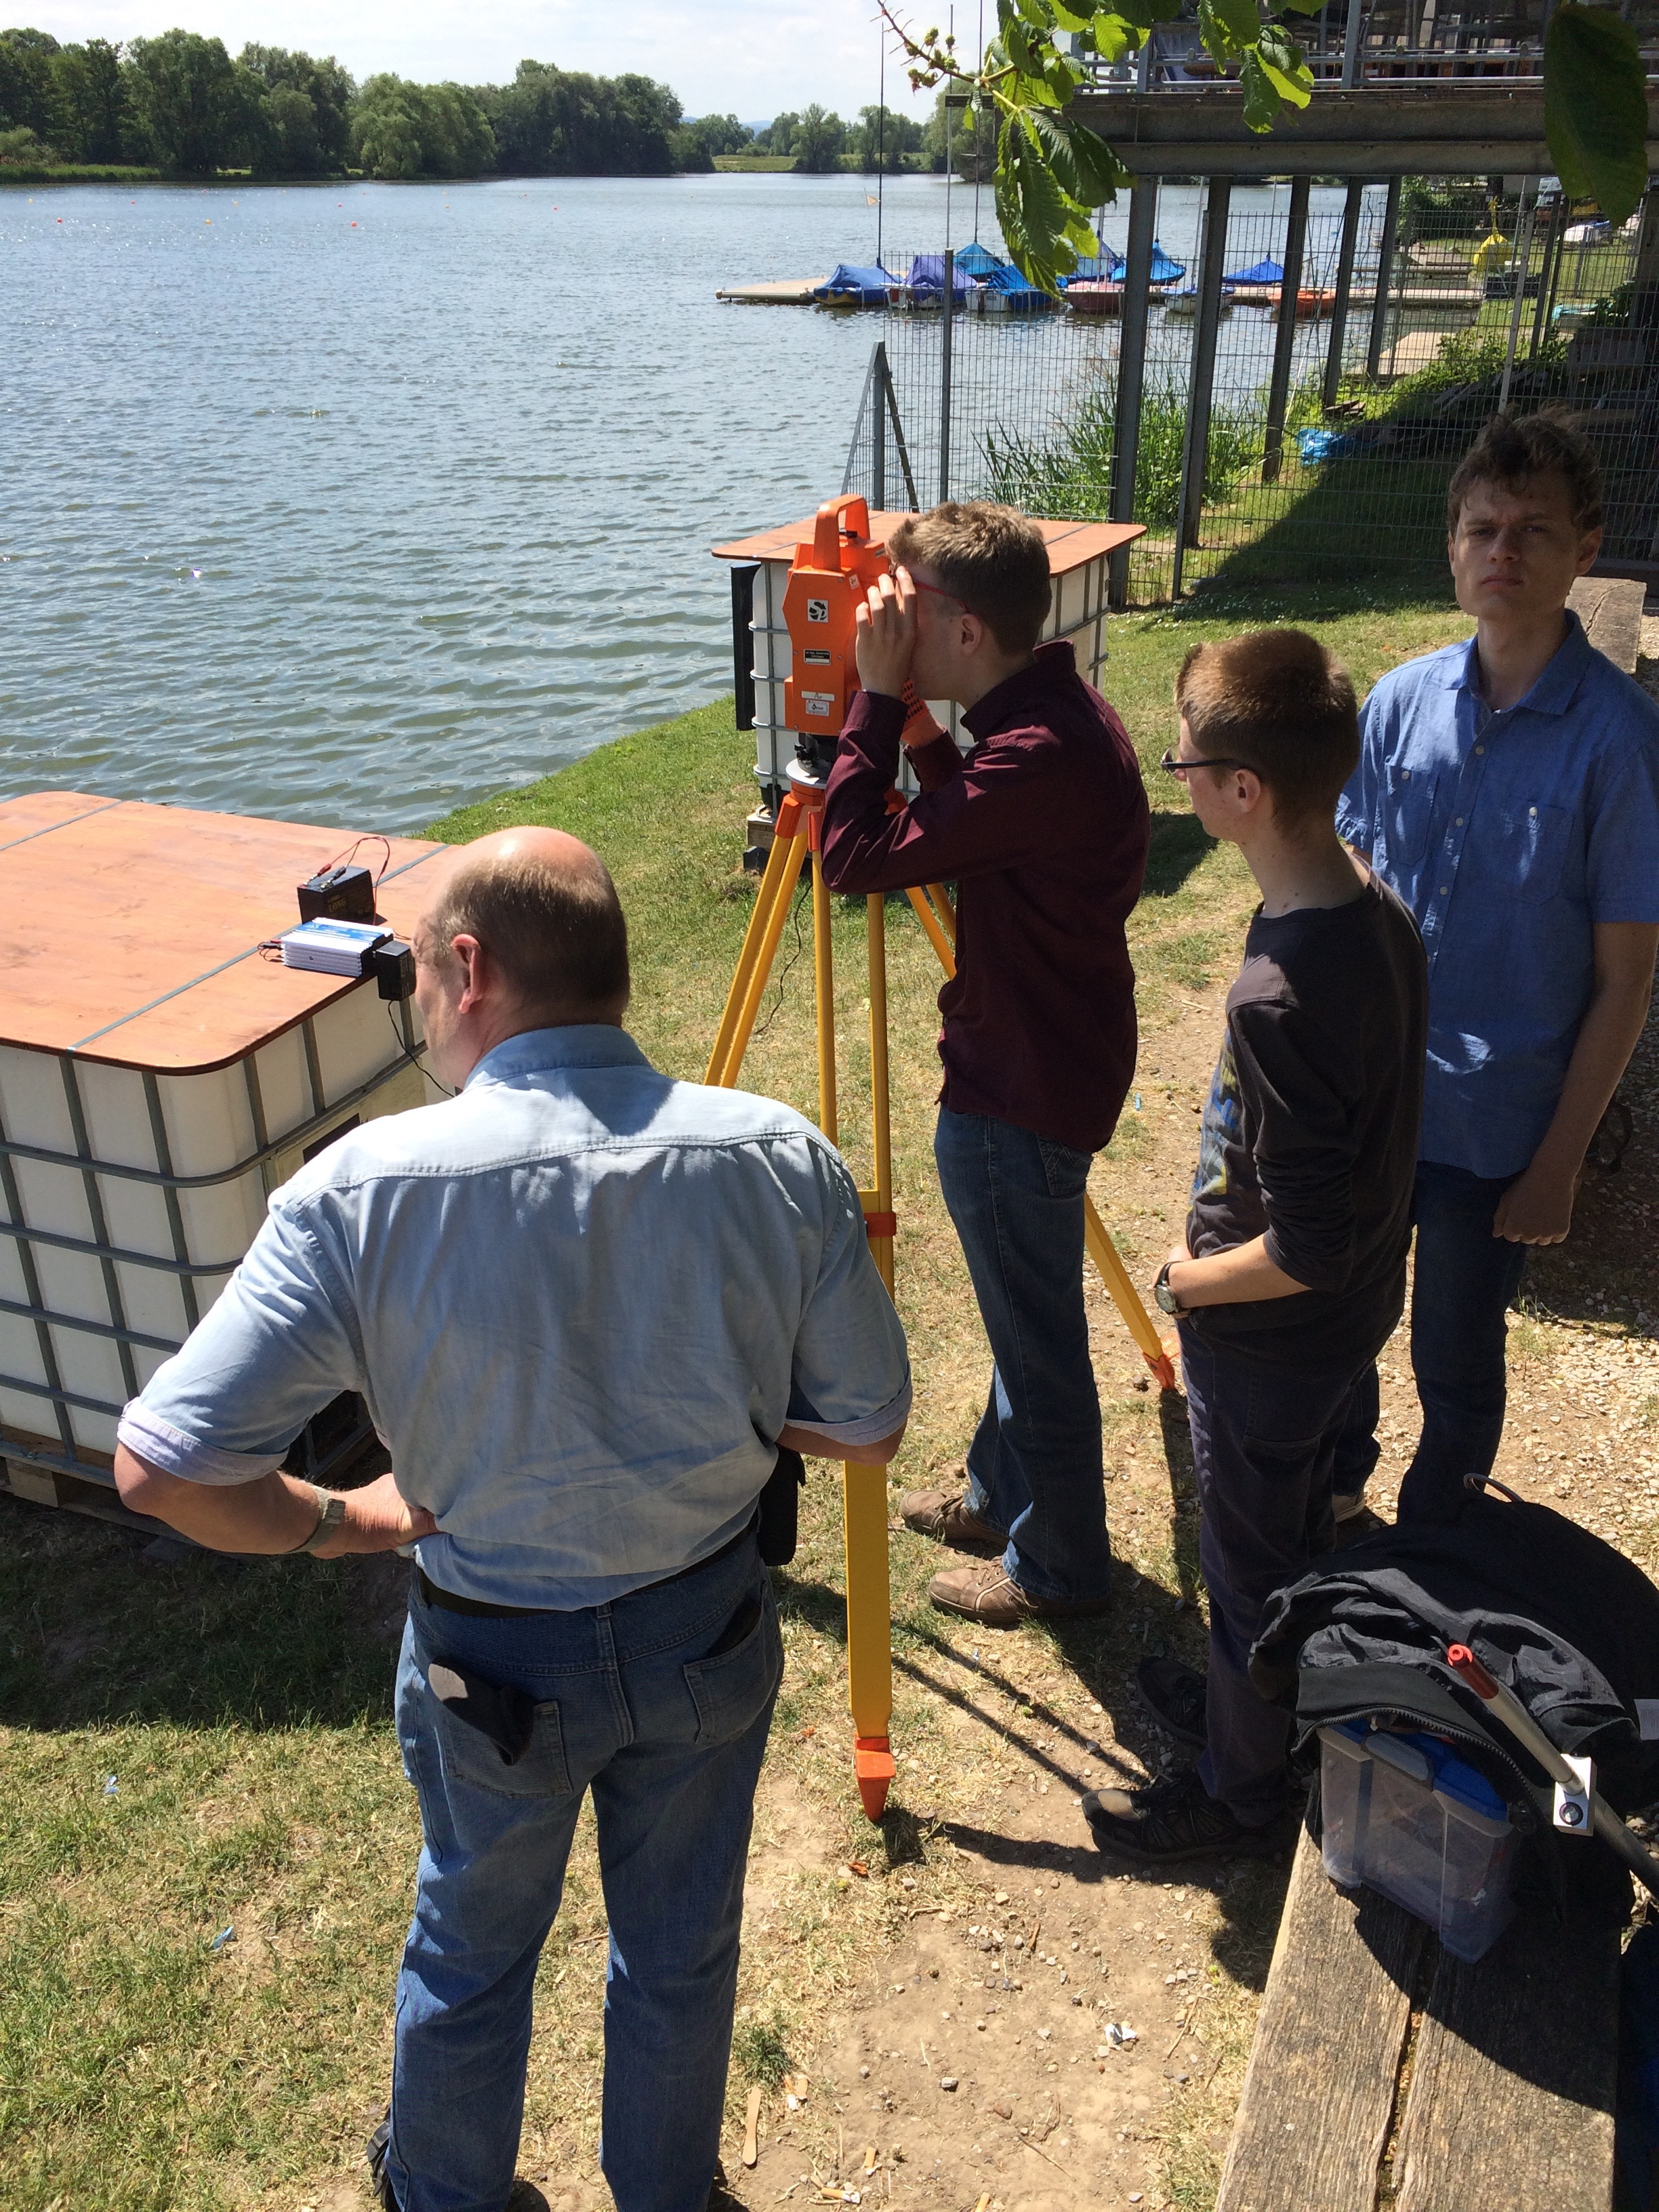
\includegraphics[height=10cm]{Geodimeter.jpg}
%	\caption{Kevin beim Einstellen des Geodimeters.}
%	\label{fig:geodimeter}
%\end{figure}


\begin{figure}[h]
	\centering
	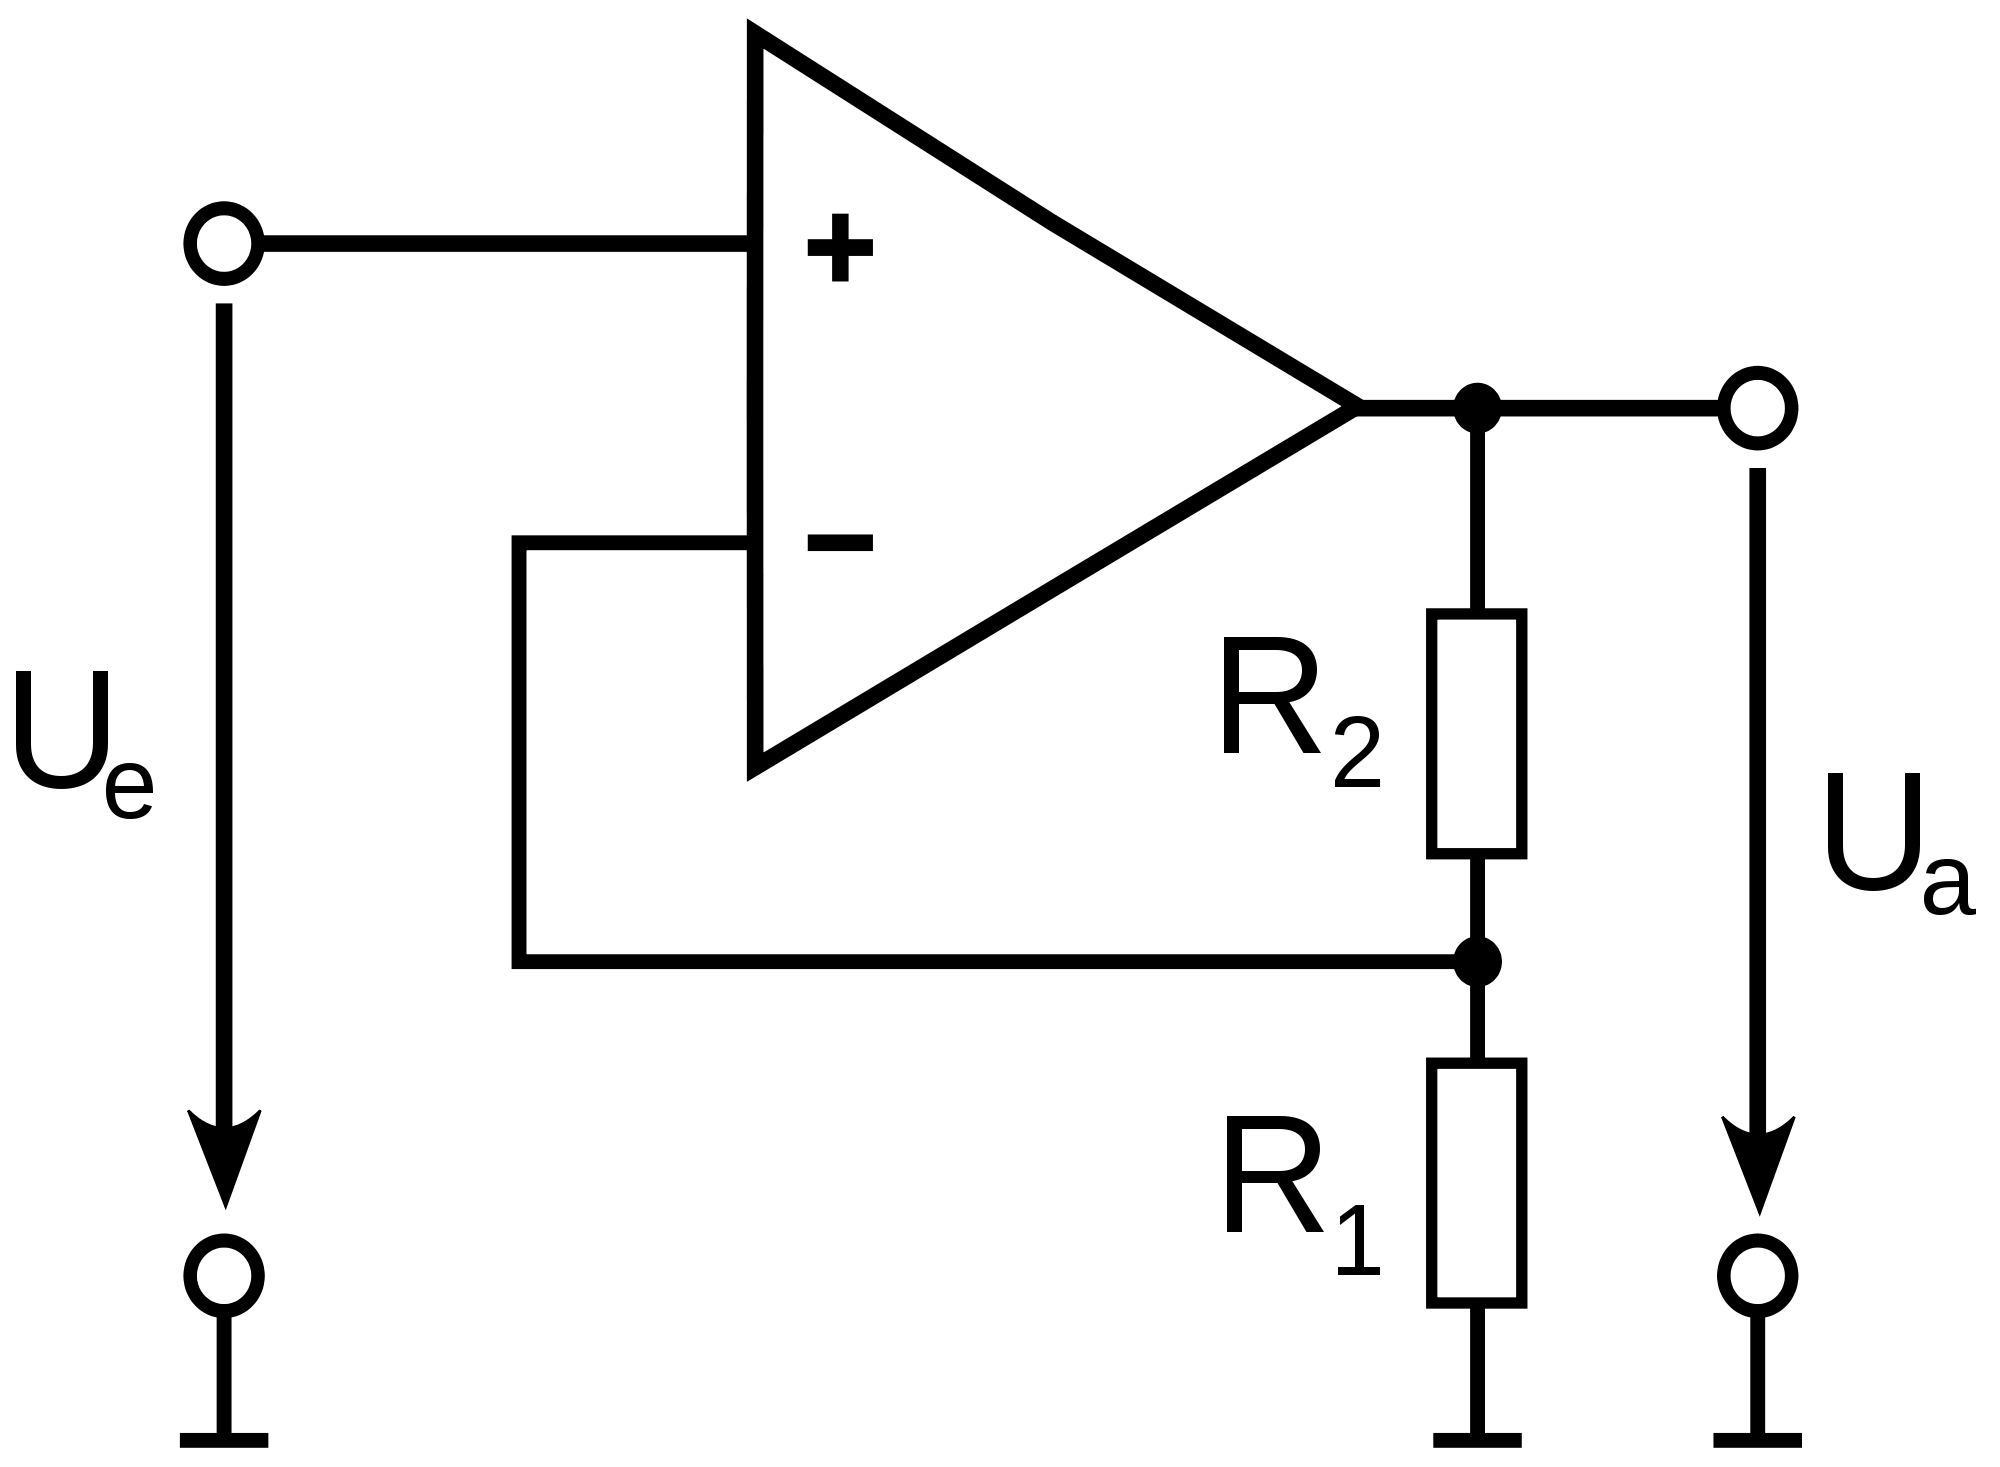
\includegraphics[width=0.6\textwidth]{nicht.png}
	\caption{\url{https://upload.wikimedia.org/wikipedia/commons/thumb/f/ff/Noninverting_Amplifier.svg/2000px-Noninverting_Amplifier.svg.png}}
	\label{fig:nicht}
\end{figure}

\end{document}
